\documentclass[11pt]{article}
\usepackage[english]{babel}
\usepackage{amsmath,amssymb,amstext}
\numberwithin{equation}{section}
\usepackage{graphicx}
\usepackage{parskip}
\usepackage{float}
\usepackage{tabularx}
\numberwithin{figure}{section}
\numberwithin{table}{section}
\usepackage{placeins}
\usepackage{esint}
\usepackage{pdfpages}
\usepackage{url}
\usepackage{array}
\usepackage{multirow}
\usepackage[
colorlinks=true,
linkcolor=black,
citecolor=black,
urlcolor=black
]{hyperref}
\usepackage[style=numeric, backend=bibtex]{biblatex}
\usepackage{todonotes}
\usepackage{subcaption}
\usepackage{multirow}
\usepackage{enumitem}
\usepackage{upgreek}
\usepackage{circuitikz}
\usepackage[labelfont=bf,labelsep=space]{caption}
\DeclareCaptionLabelSeparator{tab}{\hspace{1em}} % adjust 1em as needed
\captionsetup[figure]{labelfont=bf,labelsep=tab}

\usepackage{cleveref}
\crefname{equation}{Equation}{Equations}
\Crefname{equation}{Equation}{Equations}
\crefname{figure}{Figure}{Figures}
\Crefname{figure}{Figure}{Figures}

\renewcommand{\sectionautorefname}{Section}
\renewcommand{\subsectionautorefname}{Section}
\renewcommand{\subsubsectionautorefname}{Section}

\crefname{section}{Section}{Sections}
\Crefname{section}{Section}{Sections}
\crefname{subsection}{Section}{Sections}
\Crefname{subsection}{Section}{Sections}
\crefname{subsubsection}{Section}{Sections}
\Crefname{subsubsection}{Section}{Sections}

\addbibresource{references/references.bib}
\setlength{\textwidth}{15 true cm}
\setlength{\textheight}{22 true cm}
\oddsidemargin  0.5 cm
\evensidemargin 0.5 cm
\topmargin      0 cm

\renewcommand{\textfraction}{.2}
\renewcommand{\floatpagefraction}{.8}



\begin{document}
%\frontmatter
\pagenumbering{roman}

% Include titlepage
\begin{titlepage}	
	{\sffamily		
		\begin{center}			
			\includegraphics[width=30mm]{content/img/TU_Graz_Logo.png}
			
			\vfill\vfill\vfill
			\vfill\vfill\vfill
			
			{Simon Prato}
			% Author with existing titles
			
			\vfill\vfill\vfill
			
			{\LARGE\bfseries{Numerical Investigation of TEM Cells and Antenna Coupling}}
			% Title of the thesis			
			
			\vfill\vfill\vfill
			\vfill\vfill\vfill			
			
			{\bfseries\large{Master Thesis}}
			
			{Studies: {Electrical Engineering}}
						
			\vfill\vfill\vfill			
			
			submitted to
			
			\vfill
			
			{\bfseries\large{Graz University of Technology}}			
			
			\vfill\vfill\vfill			
			
			Supervisor
			
			{Dr. Thomas Bauernfeind}
			
			\vfill
			
			\vfill
			
			\includegraphics[width=30mm]{content/img/igte_logo.png}
			
			%% OPTIONAL: second supervisor/name of the faculty, etc.
					
			\vfill\vfill\vfill
					
			{Graz}, {February}~{2025}
			
		\end{center}
	}%% end sffamily
\end{titlepage}

\newpage

% Kurzfassung
\iftrue
\cleardoublepage
\setcounter{page}{2}
\vspace*{2.2 cm}
{\Large
\noindent
{\bf Abstract}} \\
\vspace*{0.3 cm}

Electrically small antennas that conduct high-frequency signals often generate substantial electromagnetic emissions, presenting challenges for electromagnetic compatibility. Measurement of these emissions in a TEM cell remains a widely adopted and standardized procedure. In this thesis, a comprehensive theoretical framework is developed to explain the coupling mechanisms between the antenna and the TEM cell. The proposed framework is further supported and examined through detailed numerical analyses.

In the context of these investigations, special focus is laid on electric and magnetic dipole moments, which effectively characterize electrically small radiating sources. The magnitudes of these dipole moments accurately describe the electric and magnetic coupling independently. While established measurement-based methods with the TEM cell for determining these magnitudes exists, this thesis focuses on leveraging the finite element method to eliminate potential inaccuracies arising from the measurement setup and procedure. Furthermore, this study examines near-field shielding of the antennas and their equivalent dipole moments to determine shielding efficiency of materials with different properties.

The findings presented in this thesis contribute to a deeper understanding of how the geometrical and electrical characteristics of antennas influence their coupling behavior and, consequently, the generated dipole moments. This proves useful, for example, when aiming to increase electromagnetic compatibility of an electronic system containing electrically small conducting structures. Additionally, it demonstrates how the determination of equivalent dipole moments assist in the choice of shielding material.


\noindent

% Abstract
\cleardoublepage
\fi

\selectlanguage{english}
%\listoftodos
% Inhaltsverzeichnis
	\tableofcontents  

% Tabellenverzeichnis
% optional
\newpage
	\listoffigures 

% Abbildungsverzeichnis
% optinal
\newpage
	\listoftables
	
\cleardoublepage

%\mainmatter
\pagestyle{headings}
\pagenumbering{arabic}

\section{Introduction}
% !TeX root = Documentation.tex

In recent years, electronic systems have demonstrated a clear trend toward reduced physical dimensions and increased operating speeds, consequently, higher frequencies are used. As a result, these systems often contain small conducting structures that carry currents and voltages with high amplitudes and frequencies. These structures tend to radiate and are susceptible to electromagnetic radiation, behaving as antennas and causing electromagnetic compatibility (EMC) issues.

Taking EMC into account during the design of electronic systems helps to minimize additional costs and schedule delays that may arise from potential redesigns. Furthermore, it ensures that the product operates reliably when exposed to interference from external sources \cite[p.~64]{Paul_Scully_Steffka_2023}. Consequently, research focusing on all aspects of EMC is conducted regularly. This thesis aims to contribute to these ongoing investigations, specifically through analysis of the previously mentioned small antennas and their coupling behavior in TEM cells. TEM cells are included because they provide a standardized method for measuring electromagnetic emissions under approximate free-space conditions and have been widely used for testing small devices \cites{9153508,Koepke_1989,809846}.

Several studies have analyzed the coupling behavior of small antennas and devices with TEM cells \cites{Sreenivasiah_Chang_Ma_1981, 10274360}. Specifically, \cites{Kreindl_Bauernfeind_Weiss_Stockreiter_Kaltenbacher_2024, 10742020, Wilson_1981} implement electric and/or magnetic dipole moments to model the radiated fields of such antennas, which provide information about the electric and magnetic coupling with the TEM cell, respectively. The magnitudes of the dipole moments are found by measurements with the TEM cell \cite{Sreenivasiah_Chang_Ma_1981} or numerical analysis \cite{10742020}. This thesis treats the coupling behavior of small antennas modeled with dipole moments using the latter approach, namely numerical computation using the finite element method. The advantage of this approach is the absence of inaccuracies caused by the measurement setup or related uncertainties, allowing the analysis to focus on the underlying mechanics behind the coupling behavior.

This thesis aims to explain how the electric and magnetic dipole moments of antennas are created and what factors affect them. Understanding this helps design electronic devices that meet EMC requirements and achieve specific coupling behaviors. Additionally, replacing the small antennas with their equivalent dipole moments significantly reduces computational effort, which is particularly advantageous when dealing with large computational domains.

Furthermore, this thesis investigates the shielding efficiency of different materials in the presence of dipole moments. The performance of the shielding material with respect to the electric and magnetic coupling behavior of the antennas, as reflected by the dipole moments, is investigated. The results assist in the selection of appropriate shielding material to effectively reduce emissions produced by the antennas. 

To achieve these objectives, this thesis first presents the theoretical foundations of electric and magnetic dipole moments in \cref{sec:dipole-theory}. The behavior of electromagnetic waves generated by arbitrary sources in waveguides, specifically the TEM cell, is then discussed in \cref{sec:guided-waves}. Further, background information of electromagnetic shielding and methods to determine shielding effectiveness using the TEM cell are presented. A brief overview of the finite element method is provided in \cref{sec:simulations}. 

Subsequently, \cref{sec:num-inv} addresses the numerical modeling of antennas and the TEM cell and investigates the generation of electric and magnetic dipole moments for monopole and loop antennas using the theoretical framework developed earlier. This knowledge is applied to three additional antennas, whose analysis delivers results closely related to that of the monopole and loop antennas due to their shared predominantly inductive or capacitive characteristics, which emerge as the primary distinction in the antenna coupling behavior. Equivalent circuits to model capacitive and inductive antennas, together with the TEM cell and their coupling paths, are developed, from which the dipole moments can be investigated in more detail.

\cref{sec:shielding-sim} demonstrates the application of shielding materials in numerical simulations involving dipole moments and electrically small antennas. Lastly, \autoref{sec:conclusions} presents the conclusions and discussion derived from this thesis, along with potential directions for future research.



\section{Dipole Theory}\label{sec:dipole-theory}

Magnetic and electric dipoles are an effective approach for modeling the radiation of electrically small antennas. They are defined as antennas with dimensions much less than one-tenth of the wavelength ($l\ll\lambda$)\cite[p. 151]{Balanis_1997}. By calculating the respective dipole moments, the coupling between antennas and TEM cells can be numerically estimated. This section provides a brief introduction to the underlying theory of this concept.

\subsection{Electric Dipoles}

An electric dipole is described as two tiny charged metal spheres or two capacitor-plates, which are connected with a linear wire of length $d$ and diameter $a$ \cite[p. 467]{Griffiths_2024}, \cite[p. 151]{Balanis_1997}. The charges move and accelerate along the wire, creating radiation. In case of an ideal, infinitesimal dipole, the wire is very thin ($a\ll \lambda$) and very small ($d \ll \lambda$) compared to the wavelength $\lambda$ \cite[p. 151]{Balanis_1997}, \cite[p. 468]{Griffiths_2024}. For an antenna to be accurately modeled as an infinitesimal electric dipole, its length usually must be smaller than a fiftieth of the wavelength ($d < \lambda/50$) \cite[p. 156]{Balanis_1997}. They are not very practical, but serve as a basic building block for more complex geometries. The current is spatially uniform throughout the wire.

Wires that are too long to be modeled as an infinitesimal dipole, but short enough to be considered electrically small ($\lambda / 50 < l \leq \lambda/10$), are classified as short physical dipoles \cite[pp. 162-163]{Balanis_1997}. They are a more accurate and useful representation of a linear wire antenna, and investigated further. In the remainder of this thesis, the term electric dipole refers specifically to short physical electric dipoles. Furthermore, time variation according to $\mathrm{e}^{-j\omega t}$ is assumed and therefore omitted.

A current $I_0$ is fed into the short, center-fed, linear antenna shown in \autoref{fig:electric_dipole}. The current along the antenna arms $I(z)$ linearly drops to zero \cite[p. 412]{Jackson}, as visualized in \autoref{fig:electricdipolecurrent}. Mathematically, it is described by, 

\begin{equation}
    I(z)= I_0\left( 1-\frac{2|z|}{d} \right).
    \label{eqn:current_dipole}
\end{equation}


\begin{figure}[h]
    \centering
    \includegraphics[width=0.5\linewidth]{content/10_theory/img/electric_dipole_drawing.png}
    \caption{Geometrical arrangement of a linear center-fed wire antenna.}
    \label{fig:electric_dipole}
\end{figure}

Charge accumulates along the antenna's arms. It is expressed as a charge per unit length $\rho'$ due to the thin wire. It is derived by the continuity equation,

\begin{equation}
    \rho' = \pm\frac{\mathrm{d}}{\mathrm{d}z}j\frac{ I(z)}{\omega} = \pm j\frac{2  I_0}{\omega d}.
    \label{eqn:charge_distribution_dipole}
\end{equation}

$\rho'$ is uniformly distributed along each antenna arm \cite[p. 412]{Jackson}.




An important metric is the electric dipole moment $\mathbf{p}$. It is defined as the product of charge density $\rho$ along the antenna and their source point $\mathbf{x'}$ \cite[p.410]{Jackson}, and generally expressed as 

\begin{equation}
	\mathbf{p} = \iiint_V\mathbf{x'} \rho (\mathbf{x'})\mathrm{d}\mathbf{x'}.
	\label{eqn:elec_dipole_mom}
\end{equation}

The vector $\mathbf{x}=\mathbf{\hat{a}}_x x + \mathbf{\hat{a}}_y y + \mathbf{\hat{a}}_z z$ represents the observation point coordinates, while $\mathbf{x'}=\mathbf{\hat{a}}_x x' + \mathbf{\hat{a}}_y y' + \mathbf{\hat{a}}_z z'$ represents the source point coordinates. The vectors $\mathbf{\hat{a}}_x$, $\mathbf{\hat{a}}_y$, and $\mathbf{\hat{a}}_z$ are unit vectors along the x-, y-, and z-directions, respectively. The integration is performed over the volume $V$ of the antenna.

Knowing the charge distribution $\rho'$ enables the calculation of the electric dipole moment $\mathbf{p}$ through \autoref{eqn:elec_dipole_mom}. This results in, 

\begin{equation}
    \mathbf{p}=\int_{-\frac{d}{2}}^{\frac{d}{2}}z\rho'(z)\,\mathrm{d}z\cdot\mathbf{\hat{a}}_z = j\frac{I_0d}{2\omega}\cdot\mathbf{\hat{a}}_z.
    \label{eqn:dipole_mom_example}
\end{equation}

The electric dipole moment $\mathbf{p}$ is parallel to the antenna's arms and points in the z-direction \cite[p. 412]{Jackson}, \cite[p. 155]{Griffiths_2024}. Next, the vector potential $\mathbf{A}$ is determined. It is generally defined as  \cites[p. 152]{Balanis_1997}[p. 410]{Jackson},
 
\begin{equation}
    \mathbf{A}(\mathbf{x})=\frac{\mu}{4\pi}\frac{\mathrm{e}^{-jkr}}{r}\iiint_V \mathbf{J}(\mathbf{x'})\mathrm{d}\mathbf{x'}.
    \label{eqn:vector_pot}
\end{equation}


The variable $r$ is the distance from any source point to the observation point $\left| \mathbf{x}-\mathbf{x'} \right|$. The permeability is described by $\mu$ and the term $\mathrm{e}^{jkr}$ the propagation of the wave, where $k=2\pi/\lambda$ is the propagation factor, or often called wavenumber \cite[p. 704]{Balanis_1997}. $\mathbf{J}$ is the current density in the source region. The calculations of $\mathbf{A}$ simplify to \cite[p. 410]{Jackson},

\begin{equation}
    \mathbf{A} (\mathbf{x})=-j\frac{\mathrm{\mu\omega}}{4\pi}\mathbf{p}\frac{\mathrm{e}^{-jkr}}{r}
    \label{eqn:vector_pot_elec_dipole}
\end{equation}
%Should the calculation of fields even be included? I don't need them for research. But the Field equations are important for explaining the frequency behavior of the electric dipole moment. This can be done by the radiation resistance in \autoref{eqn:elec_rad_res}. In our example, the radiation power depends on the frequency squared ($\mathbf{p}$\textasciitilde

\begin{figure}[t]
	\centering
	\includegraphics[width=0.3\linewidth]{content/10_theory/img/electric_dipole_current}
	\caption{Current distribution across linear wire antenna. It has a maximum at the feedpoint, and drops to zero at points $d/2$ and $-d/2$.}
	\label{fig:electricdipolecurrent}
\end{figure}


Any other field quantities can be derived out of the vector potential $\mathbf{A}$, such as the electric field intensity $\mathbf{E}$ and magnetic field intensity $\mathbf{H}$. This is achieved in a simpler way, when first transforming the Cartesian components of $\mathbf{A}$ into spherical ones, as demonstrated by \cite[p. 153]{Balanis_1997},

\begin{equation}
	\begin{bmatrix}
		A_r  \\
		A_\theta \\
		A_\phi
	\end{bmatrix} = 	
	\begin{bmatrix}
	\sin \theta \cos \phi & \sin \theta \sin \phi & \cos \theta\\
	\cos \theta \cos \phi &  \cos \theta \sin \phi & - \sin\theta\\
	- \sin\phi  & \cos\phi  & 0
	\end{bmatrix}
		\begin{bmatrix}
		A_x  \\
		A_y \\
		A_z
	\end{bmatrix}
\end{equation}

$\mathbf{E}$ and $\mathbf{H}$ are then expressed by \cite[p. 153]{Balanis_1997},

\begin{subequations}\label{eqn:elec_and_mag_field_dipole}
    \begin{equation}
    \mathbf{H} =\frac{1}{\mu r} \left[ \frac{\partial}{\partial r} (r A_{\theta}) - \frac{\partial A_{r}}{\partial \theta} \right]  \mathbf{\hat{\mathbf{a}}_\phi},
    \end{equation}\label{eqn:h_dipole}
    
    \begin{equation}
    \mathbf{E}=-j\omega\mathbf{A}-j\frac{1}{\omega\mu\epsilon}\nabla\left(\nabla\cdot\mathbf{A}\right).
    \end{equation}\label{eqn:e_dipole}
    
\end{subequations}

Substituting $\mathbf{A}$ into \autoref{eqn:h_dipole} and \autoref{eqn:e_dipole} reduces them to 

\begin{subequations}
	\begin{equation}
		H_r=H_\theta=0,
	\end{equation}
	\begin{equation}
		H_\phi = j\frac{k I_0 l \sin\theta}{4\pi r}\left[1 + \frac{1}{jkr}\right]\mathrm{e}^{-jkr},
	\end{equation}
\end{subequations}

and,

\begin{subequations}
	\begin{equation}
		E_r = \eta \frac{I_0 l \cos \theta}{2\pi r^2}\left[ 1 + \frac{1}{jkr} \right] \mathrm{e}^{-jkr},
	\end{equation}
	\begin{equation}
		E_\theta = j\eta \frac{kI_0 l \sin \theta }{4\pi r}\left[ 1 + \frac{1}{jkr} - \frac{1}{(kr)^2} \right] \mathrm{e}^{-jkr},
	\end{equation}
	\begin{equation}
		E_\phi = 0.
	\end{equation}
\end{subequations}


The total radiated power of the antenna is obtained by integrating the complex Poynting vector $\mathbf{W}$ over a closed surface surrounding the antenna \cite[p. 154]{Balanis_1997}. The real part of the total radiated power provides information about energy transferred by radiation, while the imaginary part about the antenna's reactive behavior. $\mathbf{W}$ is defined by 

\begin{equation}
	\mathbf{W}=\frac{1}{2}\left(\mathbf{E}\times\mathbf{H}^*\right) .
\end{equation}

The real power transfer is derived through the time-averaged Poynting vector $\mathbf{W}_\mathrm{av}$ \cite[p. 160]{Balanis_1997}, which is calculated by

\begin{equation}
    \mathbf{W}_\mathrm{av} = \frac{1}{2} \, \Re \{ \mathbf{E} \times \mathbf{H}^* \}.
    \label{eqn:time_averaged_poynting}
\end{equation}

By integrating the time-averaged real Poynting vector $ \mathbf{W}_\mathrm{av} $ over a closed surface, the radiated power $P_{\mathrm{rad}}$ is determined. The real part of the power is independent of the integrated surface, opposed to the imaginary part. In case of an electric dipole $P_{\mathrm{rad}}$ is expressed as

\begin{equation}
    P_{\mathrm{rad}} = \frac{\mathrm{c}^2\mathrm{Z_0}\mathrm{k}^4}{12\pi}|\mathbf{p}|^2.
    \label{eqn:elec_rad_res}
\end{equation}

The radiated power increases with the frequency squared, as the antenna becomes more efficient. This relation holds over the whole frequency range, as long as the antenna is electrically small.

The short physical electric dipole described in this section approximate the behavior of electrically short antennas. Special care must be taken of the excitation method and shape, as it influences the behavior \cite[p. 413]{Jackson}. Additionally, any antenna investigated through this method must remain as small as possible compared to the wavelength $\lambda$, to reduce any analytical approximation errors. 

\todo[inline]{Image theory may be added for TEM cell explanations \cite[p. 184]{Balanis}}


\subsection{Magnetic Dipoles}

The magnetic dipole is modeled as a current loop with radius $b$, whose axis is perpendicular to the plane of the loop. Its radiated fields are analogous to those of an electric dipole, with the electric and magnetic fields interchanged \cite[p. ]{Balanis_1997}. \autoref{fig:magnetic_dipole_drawing} shows a magnetic dipole.

\begin{figure}[h]
    \centering
    \includegraphics[width=0.5\linewidth]{content//10_theory//img/magnetic_dipole_drawing.png}
    \caption{Magnetic dipole}
    \label{fig:magnetic_dipole_drawing}
\end{figure}

The magnetic dipole moment is given by \autoref{eqn:mag_dipole_moment}.

\begin{equation}
    \mathbf{m}=\frac{1}{2}\int (\mathbf{x} \times \mathbf{J})\mathrm{d}^3x
    \label{eqn:mag_dipole_moment}
\end{equation}

A magnetic dipole can be represented with a current loop, or a magnetic current along a straight path. \autoref{eqn:magn_current_curr_loop} shows the mathematical relation between these two \cite{Balanis_1997}. 

\begin{equation}
    I_m L = \mathrm{i}S\omega\mu_0 I_0
    \label{eqn:magn_current_curr_loop}
\end{equation}

$I_m$ is the magnetic current with the unit $\mathrm{V}$. The area $S$ of the loop is calculated by $b^2\pi$. $I_0$ is the electric current with the unit $\mathrm{A}$ flowing through the loop, and $\mu_0$ is the permeability of free space.

\todo{Add fields and radiation power formulas, if it is needed later}

\subsubsection{Crossed Dipoles}
% Read Bauernfeind's: Crossed Dipole Antennas

% When placing the magnetic dipole in the center of the upper or lower chamber of the TEM cell, and pointing in y-direction, it will generate a TEM-wave. Same goes for the electric dipole, pointing in z-direction. When combining two of these dipole moments, any excitation with the first order TEM mode is possible. This is the main idea for modeling antennas. The relation of the magnetic and electric fields is assumed to be roughly equal to the free space wave impedance. Also, magnetic dipoles create a difference in output voltage of the two ports, while electric dipoles create a increase of voltage in both ports. The power transmitted is the same. However: How are they modeled in HFSS? 

Crossed dipoles can generate a wide variety of radiation patterns. Supposed two dipoles are placed perpendicular to each other and fed 90° out of phase, an omnidirectional radiation pattern in created \cite{7293591}. If the equivalent dipoles of an EUT represents such two dipoles, any mode which can propagate in the TEM cell will do so, and therefore influence the measurement result. It is therefore not only important to know which dipoles there are representing the EUT, but also what phase and magnitude they have. Meaning that not only the dipoles aligned with the TEM mode alone influence the result. 
\todo{Write}

\todo{Dipoles next to conducting planes (balanis, collin)}

% Also, the reflections of the conducting sheets of the TEM cell might enhance the dipoles' gain, therefore artificially supporting a certain mode even more. This property is often used in antennas, where a perfect electric conductor (PEC) is placed a quarter wavelength away from the antenna, hence enhancing the gain \cite{7293591}. 


\input{content/10_dipoles/12_fields}

\section{Guided Waves}\label{sec:guided-waves}
\subsection[Lorentz Reciprocity Theorem]{Lorentz Reciprocity Theorem\protect\footnote{This section follows closely the treatment in: Robert E. Collin, \textit{Field Theory of Guided Waves}, IEEE Press, 2015 and Constantine A. Balanis, \textit{Antenna theory: Analysis and design}, Wiley, 1997.}}\label{sec:lorentz_theorem}


Let two source pairs $\mathbf{J}_1$, $\mathbf{M}_1$ and $\mathbf{J}_2$, $\mathbf{M}_2$ exist in a volume $V$, bounded by the closed surface $S$. The medium in $V$ is linear and isotropic. The source pairs generate fields $\mathbf{E}_1$, $\mathbf{H}_1$ and $\mathbf{E}_2$, $\mathbf{H}_2$, respectively, with the same frequency. The fields and source pairs can then be related with \cites[p.~145]{Balanis_1997}[p. 49]{Collin_2015}

\begin{equation}
	-\nabla \cdot (\mathbf{E}_1\times \mathbf{H}_2-\mathbf{E}_2\times \mathbf{H}_1)=\mathbf{E}_1\cdot \mathbf{J}_2+\mathbf{H}_2\cdot \mathbf{M}_1-\mathbf{E}_2\cdot \mathbf{J}_1-\mathbf{H}_1\cdot \mathbf{M}_2.
	\label{eqn:lorentz_rec_theorem}
\end{equation}

Integrating \autoref{eqn:lorentz_rec_theorem} over $V$, and converting the volume integral to a surface integral with the divergence theorem, leads to \cites[p. 145]{Balanis_1997}[p. 50]{Collin_2015}

\begin{align}
    -\oiint_S &(\mathbf{E}_1\times \mathbf{H}_2-\mathbf{E}_2\times \mathbf{H}_1)\cdot d\mathbf{s}'\nonumber\\&=\iiint_V
\left(\mathbf{E}_1\cdot \mathbf{J}_2+\mathbf{H}_2\cdot \mathbf{M}_1-\mathbf{E}_2\cdot \mathbf{J}_1-\mathbf{H}_1\cdot \mathbf{M}_2\right)\cdot dv'.
    \label{eqn:lorentz_rec_theorem_int}
\end{align}

This integral equation relates the coupling of different source points. Additionally, if one of these sources is set to zero, the respective source point can serve as an observation point. Setting all sources to zero allows investigation of the coupling of modal fields in a waveguide to other modes, as the following example shows. Suppose the volume $V$ does not contain sources $\mathbf{J}_1 = \mathbf{M}_1 = \mathbf{J}_2 = \mathbf{M}_2 = \mathbf{0}$. Then, the source-free Lorentz Reciprocity theorem reduces to the condition that the modes in the waveguide must fulfill \cite[pp. 145-146]{Balanis_1997}: 

\begin{subequations}
	\begin{equation}
		\nabla \cdot (\mathbf{E}_1\times \mathbf{H}_2-\mathbf{E}_2\times \mathbf{H}_1)=0,
	\end{equation}
	\begin{equation}
		\oiint_S (\mathbf{E}_1\times \mathbf{H}_2-\mathbf{E}_2\times \mathbf{H}_1)\cdot d\mathbf{s}'=0.
		\label{eqn:modes_waveguide}
	\end{equation}
\end{subequations}

Another application arises when investigating a volume $V$ confined by a perfectly conducting surface $S$, in which the linear current densities $\mathbf{J}_1$ and $\mathbf{J}_2$ flow. Because $\mathbf{n}\times\mathbf{E}_1=\mathbf{n}\times\mathbf{E}_2=0$ along the surface $S$, the surface integral in \autoref{eqn:lorentz_rec_theorem_int} vanishes, leading to  

\begin{equation}
	\mathbf{E}_1\cdot\mathbf{J}_2=\mathbf{E}_2\cdot\mathbf{J}_1.
\end{equation}

This is the Rayleigh-Carson form of the Lorentz reciprocity theorem \cite[p. 50]{Collin_2015}. It states that the component of $\mathbf{E}_1$ along $\mathbf{J}_2$ is equal to the component of $\mathbf{E}_2$ along $\mathbf{J}_1$, and vice versa \cite[p. 50]{Collin_2015}. 

In summary, the Lorentz Reciprocity theorem is useful for deriving reciprocal aspects of waveguides, finding orthogonal properties of modes, investigating fields generated by currents and dipole moments in waveguides \cite[p. 50]{Collin_2015}, among several other examples. This theorem will be employed often throughout the remainder of this thesis.

\subsection{Green's Function}

\subsubsection{Scalar Green's Function}\label{sec:scal_green}

Green's function describes the response of a linear differential operator $L$ to a point source as an input, which is modeled by delta-function $\delta$. Its general form is 

\begin{equation}
    \mathrm{L}G(\mathbf{x},\mathbf{x'}) = \delta(\mathbf{x}-\mathbf{x'}).
    \label{eqn:general_greens_funct}
\end{equation}

Once \autoref{eqn:general_greens_funct} is solved and the Green's function $G$ of this specific operator is known, it can be used to solve any input function, such as $u(\mathbf{x})$ in 

\begin{equation}
    Lu(\mathbf{x}) = f(\mathbf{x}).
    \label{eqn:examplary_function_with_operator}
\end{equation}

\todo{What is f(x)?}

This is done by a convoluting 

\begin{equation}
    u(\mathbf{x})=\iiint_V G(\mathbf{x},\mathbf{x'})f(\mathbf{x'})\mathrm{d}\mathbf{x'}
    \label{eqn:examplary_function_solved}
\end{equation}

The Green's function can be used to solve equations involving the Nabla operator $\nabla$ in electrostatics. \autoref{eqn:greens_function_scalar_pot_1} and \autoref{eqn:greens_function_scalar_pot_2} demonstrate how the scalar potential $\phi$ can be calculated from point charge distributions in space $\rho$ by using the Green's function of the Nabla operator. There, the Green's function $G(\mathbf{x},\mathbf{x'}) = \frac{1}{4\pi |\mathbf{x}-\mathbf{x'|}}$ represents the potential at position $\mathbf{x}$ created by an unit point charge at point $\mathbf{x'}$.

\begin{subequations}
\begin{equation}
    \nabla \phi = -\frac{\rho}{\epsilon_0}
    \label{eqn:greens_function_scalar_pot_1}
\end{equation}
\begin{equation}
    \phi(\mathbf{x}) = \frac{1}{4\pi\epsilon_0}\iiint_V\frac{\rho(\mathbf{x'})}{|\mathbf{x}-\mathbf{x'}|}\mathrm{d}V'
    \label{eqn:greens_function_scalar_pot_2}
\end{equation}
\end{subequations}

When boundary conditions are present, the Green's Function may be modified to make the boundary condition vanish. The resulting function is called tailored Green's Function. This proves especially useful in the analysis of guided waves. Another possibility is to construct the Green's Function by a series of reflections on boundaries, applying image theory on perfectly conducting surfaces \cite{Collin_2015}.


%This enables an expansion of the fields in a waveguide excited by an internal source. The perfectly conducting surfaces of the waveguides mirror the source infinitely often. Therefore, the Green's function may be represented by a series of these mirror sources. In practice, these calculations are cumbersome, and only the most significant parts of the series are computed \cite{Collin_2015}. %Should I show mathematical calculations?


\subsubsection{Dyadic Green's Function}\label{sec:dyad_green}

The scalar Green's Function demonstrated in \autoref{sec:scal_green} is useful to solve for one-dimensional functions. However, for the analysis of waveguides, the calculation of the three-dimensional vector potential $\mathbf{A}$ as in \autoref{eqn:helmholtz} is necessary.  

\begin{equation}\label{eqn:helmholtz}
	\nabla^2\mathbf{A}+k^2\mathbf{A}=-\upmu \mathbf{J}
\end{equation}


When replacing $\upmu \mathbf{J}$ by an unit vector source, the solution of the differential equation is shown in \autoref{eqn:sol_dyadic_green}. This is a vector Green's Function by definition.

\begin{equation}\label{eqn:sol_dyadic_green}
	(\mathbf{a}_x + \mathbf{a}_y + \mathbf{a}_z) \frac{e^{-j k |\mathbf{r} - \mathbf{r}_0|}}{4\pi |\mathbf{r} - \mathbf{r}_0|}
\end{equation}

The solution of any current distribution $\mathbf{J}$ can be obtained by superposition, analogous to the scalar Green's Function. A prerequisite is that each component of the current vector $\mathbf{J}$ is each associated with one unit vector of the Green's function, i.e. $J_x$ with $\mathbf{a_x}$, $J_y$ with $\mathbf{a_y}$ and $J_z$ with $\mathbf{a_z}$. This is implemented by using a dyadic Green's Function $\mathbf{\hat{G}}$. The dyadic has a mapping function, rather than an operational one. The dyadic Green's Function is defined as the solution of \autoref{eqn:helmholtz_green}.

\begin{equation}\label{eqn:helmholtz_green}
	\nabla^2 \mathbf{\hat G}(\mathbf{r}, \mathbf{r}_0) + k^2 \mathbf{\hat G} = -\mathbf{\hat I} \delta(\mathbf{r} - \mathbf{r}_0)
\end{equation}

Analogous to the scalar Green's Function, multiplying the unit input function by $\mathbf{\hat{I}}$ leads to the same multiplication of the Green's function, as shown in \autoref{eqn:dyadic_final}.

\begin{equation}\label{eqn:dyadic_final}
	\mathbf{\hat G}(\mathbf{r}, \mathbf{r}_0) = \mathbf{\hat I} \frac{e^{-jk|\mathbf{r} - \mathbf{r}_0|}}{4\pi |\mathbf{r} - \mathbf{r}_0|}
\end{equation}

The dyadic Green's Function is commonly applied to calculate field distributions in waveguides. In \cite{Wilson_1981} it is used to derive the fields in a TEM cell caused by a vertical current conducting wire with help of the small-gap approximation.




\subsection{Modes in TEM Cells}\label{sec:modes_tem_cell}
\subsubsection{Power transfer of modes}
% Goal is to describe the modes in a TEM cell, including their cut-off frequencies. \cite{Kreindl_Bauernfeind_Weiss_Stockreitner_Kaltenbacher_2024} shows that these investigations are important. There are also modes propagating perpendicular to the intended propagation direction. Why are no waveguides used? Explain.

% In this paper, a VCSEL with a decoupling capacitor are modeled. It is visible, that the electric coupling dominates at an orientation of 90°. A local minimum is then visible. At 400\,MHz and upwards, inductive coupling becomes dominant, but only at 0° where it couples with the septum. It is possible, that a certain mode can propagate at a certain frequency, which influenced the result in this paper. 


Any electromagnetic field distribution in a waveguide can be represented by an infinite series of normal modes. \autoref{eqn:norm_power} shows that each mode is orthogonal to each other, with $\mathbf{e_n}^\pm$ and $\mathbf{h_n^\pm}$ being the function vectors of the electric and magnetic field in transverse direction \cite{Collin_2015}. A coupling between the modes only occurs due to geometric changes of the waveguide. Additionally, each mode is normalized to $\sqrt{\mathrm{W}}$, shown by \autoref{eqn:unit_power}. Only the transverse fields are investigated in these Equations, because they carry power along the waveguide, opposed to the fields in the propagation direction.

\begin{align}
    \iint \mathbf{e_n^\pm}\times \mathbf{h_m^\pm}\mathrm{d}S\mathbf{n}&=0 \quad\text{if}\quad n\neq m
    \label{eqn:norm_power}\\
    \iint \mathbf{e_n^\pm}\times \mathbf{h_n^\pm}\mathrm{d}S\mathbf{n}&=1
    \label{eqn:unit_power}
\end{align}

The radiated fields can be described by a summation of normal modes, as in \autoref{eqn:modal_superposition1} and \autoref{eqn:modal_superposition2}. The coefficients of these modes are straightforward to calculate, due to Lorentz Reciprocity Theorem, if the waveguide's walls are perfectly conducting. Ideally, any higher order mode than the first TEM mode will be suppressed, and the calculation simplifies to $n=0$. Additionally, it is assumed that the source is electrically small, which makes it possible to represent it with dipoles, further simplifying the equations \cite{Koepke_1989}. 

\begin{align}
    \mathbf{E^\pm}&=\sum_na_n\mathbf{E_n^\pm}    \label{eqn:modal_superposition1}\\
    \mathbf{H^\pm}&=\sum_na_n\mathbf{H_n^\pm}    \label{eqn:modal_superposition2}
\end{align}

Suppose a current source $\mathbf{J_1}$ excites a waveguide (as is the case with the dipoles in the TEM cell). Normally, such a current source would be driven with external fields, but for the sake of the argument, they are ignored. Only $\mathbf{E}$ and $\mathbf{H}$ are considered, which are the fields radiated by $\mathbf{J_1}$. Additionally, $\mathbf{E}_n^\pm$ and $\mathbf{H}_n^\pm$ are the resulting waveguide fields, with the signs indicating the direction of propagation. Take \autoref{eqn:lorentz_rec_theorem_int} and set $\mathbf{J_2}=\mathbf{M_1}=\mathbf{M_2}=0$. Now, only the current source $\mathbf{J_1}$ remains, and the \autoref{eqn:J1_propagating_waves} emerges. % Explain how certain surfaces do not to have be integrated, therefore rendering this equation very useful. Also, the expansion coefficients can be determined. Maybe do this calculation with a rectangular waveguide.

\begin{equation}
    \oiint _S (\mathbf{E_n^\pm}\times \mathbf{H}-\mathbf{E}\times \mathbf{H}_n^\pm)\cdot\mathrm{d}\mathbf{S}=\iiint \mathbf{J_1}\cdot\mathbf{E_n^\pm}\mathrm{d}V
    \label{eqn:J1_propagating_waves}
\end{equation}

\begin{figure}[t]
	\centering
	\includegraphics[width=0.7\linewidth]{content/img/reciprocity_tem_cell}
	\caption{TEM cell with an arbitrary current source $\mathbf{J}$ along the curve $\mathbf{\tau}$. $\mathbf{E}$ and $\mathbf{H}$ are the field intensities induced by the current. $\mathbf{E}^+$ and $\mathbf{E}^-$ are outgoing fields towards both output ports of the TEM cell. $\mathbf{S}$ indicates the surface, and $V$ the volume of the domain in question.}
	\label{fig:reciprocitytemcell}
\end{figure}


In case of the TEM cell, it is desirable that only the TEM mode is propagating, and that the source is represented by a dipole. When the expansions \autoref{eqn:modal_superposition1}, \autoref{eqn:modal_superposition2} and the orthogonal property \autoref{eqn:norm_power} are used, and when considering an electric dipole, the \autoref{eqn:dipole_tem_waves} arises. In this equation, the wave amplitudes $a$ and $b$ are given through the surface integral in the Lorentz Reciprocity theorem, with $a$ being the wave going to the left side, and $b$ to the other. The electric dipole moment $\mathbf{m_e}$ is given by the current $\mathbf{J}$ flowing through the infinitesimal wire. Note that only the electric field of TEM wave propagation is considered. In reality, more modes may propagate, for which the electric field must be replaced by the superposition of normal modes as in \autoref{eqn:modal_superposition1}. %Additionally, to calculate the exact value of the electric field, a series of image sources as a Green's function may be applied.

\begin{equation}
\begin{pmatrix}a \\b\end{pmatrix} = -\frac{1}{2}\mathbf{m_e}\cdot \mathbf{E}^\pm
\label{eqn:dipole_tem_waves}
\end{equation}
\todo{$E_n^\pm$?}

If this arbitrary current distribution forms an infinitesimal loop, the source can be represented by a magnetic dipole moment $\mathbf{m_m}$. It is defined by the product $\mathbf{m_m}=\mathbf{A}\cdot I$, an infinitesimal current loop with area $A$ carrying a current $I$. This leads to \autoref{eqn:mag_dipole_moment_tem}. This formulation assumes, that the magnetic field strength $\mathbf{H}^\pm$ does not change over the loop area, i.e. the loop is electrically small. Otherwise, the magnetic field strength $\mathbf{H}^\pm$ must be considered in the integration \cite{Collin_2015,Sreenivasiah_Chang_Ma_1981}.

\begin{align}
    \begin{pmatrix}a \\b\end{pmatrix} &= -\oint_C \mathbf{E}^\pm \mathrm{d}l \nonumber \\
    &= -\iint_{S_0} \nabla \times \mathbf{E}^\pm \mathrm{d}\mathbf{S}\nonumber\\
    &= \mathrm{i}\omega\mu_0\iint_{S_0} \mathbf{H}^\pm\cdot \mathrm{d}\mathbf{S}\nonumber\\
    &= \mathrm{i}\omega\mu_0\mathbf{m}_m\mathbf{H}^\pm 
    \label{eqn:mag_dipole_moment_tem}
\end{align}


If there are several modes propagating, it is useful to find the coefficients of the modes $a_n$ and $b_n$ in \autoref{eqn:modal_superposition1} and \autoref{eqn:modal_superposition2}. In this case, the orthogonality property in \autoref{eqn:norm_power} is used to derive \autoref{eqn:an} and \autoref{eqn:bn} \cite{Collin_2015}. The wire is described by a curve C, and the tangential vector $\boldsymbol{\tau}$ is used to integrate along this curve.

\begin{subequations}
    \begin{equation}
        2a_n = -\int_C \boldsymbol{\tau}\cdot\mathbf{E}_n^-\mathrm{d}l
        \label{eqn:an}
    \end{equation}
        \begin{equation}
        2b_n = \int_C \boldsymbol{\tau}\cdot\mathbf{E}_n^+\mathrm{d}l
        \label{eqn:bn}
    \end{equation}
\end{subequations}

\subsubsection{Modes in rectangular waveguides}

A TEM cell is used for EMC test specifications. It makes the conduction of TEM waves possible, which resemble planar free-space waves. Additionally, it shields the waves from radiating to the sides, for which it has a clear advantage to a stripline \cite{809846,990711}. A simple rectangular waveguide cannot be used for this application. Assuming that a monochromatic wave travels down the waveguide, the waves will propagate without dampening only at a certain angle of reflection on the perfectly conducting surface. A short mathematical proof can be shown here, using Maxwell's equation. It shows that the electric and magnetic fields in direction of propagation cannot both be zero. 
\begin{align}
    \mathbf{E}&=(E_{0,x}\cdot\mathbf{e_x}+E_{0,y}\cdot\mathbf{e_y}+E_{0,z}\cdot\mathbf{e_z})\mathrm{e}^{\mathrm{i}(\omega t-kz)}\\
    \mathbf{H}&=(H_{0,x}\cdot\mathbf{e_x}+H_{0,y}\cdot\mathbf{e_y}+H_{0,z}\cdot\mathbf{e_z})\mathrm{e}^{\mathrm{i}(\omega t-kz)}\\
    \nabla \times \mathbf{E} &=\begin{pmatrix}\frac{\mathrm{d}}{\mathrm{d}y}E_z-\mathrm{i}kE_y \\\mathrm{i}kE_x-\frac{\mathrm{d}}{\mathrm{d}x}E_z \\\frac{\mathrm{d}}{\mathrm{d}x}E_y-\frac{\mathrm{d}}{\mathrm{d}y}E_x\end{pmatrix}=\begin{pmatrix} -\mathrm{i}\omega B_x\\-\mathrm{i}\omega B_y\\ -\mathrm{i}\omega B_z \end{pmatrix}\\
    \nabla \times \mathbf{B} &=\begin{pmatrix}\frac{\mathrm{d}}{\mathrm{d}y}B_z-\mathrm{i}kB_y \\\mathrm{i}kB_x-\frac{\mathrm{d}}{\mathrm{d}x}B_z \\\frac{\mathrm{d}}{\mathrm{d}x}B_y-\frac{\mathrm{d}}{\mathrm{d}y}B_x\end{pmatrix}=\begin{pmatrix} \frac{\mathrm{i}\omega}{\mu\epsilon} E_x\\\frac{\mathrm{i}\omega}{\mu\epsilon} E_y\\ \frac{\mathrm{i}\omega}{\mu\epsilon} E_z \end{pmatrix}
\end{align}

If $E_z$ and $B_z$, the fields in direction of propagation, were both zero, then the change of the transverse fields would be constantly zero, and because of the boundary conditions, all transverse fields would be zero. \autoref{eqn:rect_waveguide_gauss} shows Gauss' law and \autoref{eqn:rect_waveguide_faraday} Faraday's law if $E_z=B_z=0$, from which the unchanging transverse electric field can be derived. 

\begin{align}
    \frac{\mathrm{d}}{\mathrm{d}x}E_x+\frac{\mathrm{d}}{\mathrm{d}y}E_y&=0\quad\text{Derived out of Gauss' law}\label{eqn:rect_waveguide_gauss}\\
    \frac{\mathrm{d}}{\mathrm{d}y}E_x-\frac{\mathrm{d}}{\mathrm{d}x}E_y&=0\quad\text{Derived out of Faraday's law}\label{eqn:rect_waveguide_faraday}
\end{align}

\subsubsection{TEM Mode in TEM Cells}

A TEM cell solves this problem, by having a gap between the septum and the side walls. Essentially, it can be considered as two rectangular waveguides with apertures on the sides. Those apertures allow perturbations of the electromagnetic fields between them. The boundary conditions of the Laplace equation now changed due to the gaps. The Green's function may be calculated of the new construction, now considering the boundary conditions at the gaps, which must be the same for both waveguides (to prevent discontinuities). In the papers of Tippet, Chang and Wilson, this new Green's function lead to the excitation of TEM modes in both waveguides \cite{Tippet_Chang_Crawford_1976,Wilson_1981}. However, the gap is assumed to be small, electrically ($\xi g \ll 1$) and compared to the septum width ($g/a \ll 1$) \cite{4091747}. The variable $\xi=\sqrt{k_0^2 - \beta ^2}$ is the transverse (in y-direction) propagation constant, and consists of the free-space wave number $k_0$ and longitudinal (in z-direction) propagation constant $\beta$. The variables $g$ and $a$ are geometry variables of the TEM cell annotated in \autoref{fig:verticalantennatemcell}.

\begin{figure}[h]
	\centering
	\includegraphics[width=0.7\linewidth]{content/img/vertical_antenna_tem_cell}
	\caption{TEM cell with vertical antenna inserted}
	\label{fig:verticalantennatemcell}
\end{figure}


To analyze the fields in a TEM cell, the dyadic Green's function discussed in \autoref{sec:dyad_green} proofs itself to be useful. It is assumed, that a vertical, electrically short antenna is inserted in the top center of the TEM cell. This is modeled by a current distribution in y-direction $\mathbf{\hat J}(\mathbf{x}) = \mathbf{a}_y J(\mathbf{x})$ \cite{4091747}. Accordingly, the Green's function reduces to $\mathbf{\hat G}(\mathbf{x, x'}) = \mathbf{a}_y G(\mathbf{x, x'})$. \todo{Check Vector notation. Is correct for Dyadics?} First, the Green's function for a rectangular waveguide $G_O(\mathbf{x,x'})$ is shown in \autoref{eqn:unperturbed_green} \cite{Balanis_1997}. There, $\eta_0$ is the free-space impedance, $M=m\pi / (2a)$, $N=n\pi/b$ and $K_m=(\xi^2-M^2)^{1/2}$. Furthermore,

$\Delta_n = 
\begin{cases}
	\frac{1}{2}, & n = 0 \\
	1,           & n > 0
\end{cases} $ 

and,

$g_{mn}(\mathbf{x}_t, \mathbf{x}_t') = \left( \frac{2}{ab} \right)
\sin M(x + a) \sin M(x' + a)
\cdot \cos Ny \cos Ny'$

are functions implemented in \autoref{eqn:unperturbed_green}. The components $x$, $x'$ and $y$, $y'$ are part of the vectors $\mathbf{x}_t$, $\mathbf{x}'_t$. 

\begin{equation}\label{eqn:unperturbed_green}
	\tilde{G}_0(\mathbf{x}_t, \mathbf{x}_t') =
	\frac{-\mathrm{j} \eta_0}{k_0} \left\{\sum_{m,n=0}^{\infty} \frac{\Delta_n [M^2 + \beta^2]}{M^2 + N^2 - \xi^2} \; g_{mn}(\mathbf{x}_t, \mathbf{x}_t')
	\right\}
\end{equation}


The TEM cells Green's function by adding a unperturbed term to it \cite{4091747}. The derivation of those Green's Functions is demonstrated in \cite{Wilson_1981}, which uses the same methods described in \cite{Balanis_1997}, as mentioned above.

The perturbed term in \autoref{eqn:perturbed_green} describes the influence of the gaps on the field distribution. They are derived by forcing the tangential fields to be continuous across the gaps, then describing this boundary condition mathematically as a perturbing second Green's function. The rest of the boundary conditions on the are zero due to the geometry of the TEM cell. The functions used are,

\begin{equation*}
L(\beta) = \left[
\ln \left( \frac{8a}{\pi g} \right)
- \frac{\pi}{a} \sum_{m \in \{1,3,5,...\}}^{\infty} \left(
\frac{\cot K_m b}{K_m}
+ \frac{2a}{m\pi}
\right)
\right]^{-1}
\end{equation*}

and, 

\begin{equation*}
f(\mathbf{x}_t) = \sum_{m \in \{1,3,5,...\}}^{\infty} M \frac{\cos K_{m} (b - y)}{K_{m} \sin K_{m} b}
\sin Ma \cos Mx J_0(Mg).
\end{equation*}

To receive the final Green's Function, the unperturbed and perturbed term are added together ${G}(\mathbf{x}_t, \mathbf{x}'_t) = {G}_O(\mathbf{x}_t, \mathbf{x}'_t)+{G}_g(\mathbf{x}_t, \mathbf{x}'_t)$. Naturally, the observation point $\mathbf{x}$ can only be on the upper half in the chamber, where the source is also located \cite{4091747}. 


\begin{equation}\label{eqn:perturbed_green}
	\widetilde{G}_g(\mathbf{x}_t, \mathbf{x}'_t) = \frac{ -j \pi k_0 \eta_0}{2 a^2 s^2} L(\beta) f(\mathbf{x}_t) f(\mathbf{x}'_t)
\end{equation}

Because waves propagating in the TEM cell are assumed to travel into infinity, they might have any longitudinal propagation constant $\beta$. They are not limited by boundary conditions in this direction. It therefore proofs useful to apply a Fourier Series over this variable, as done in \autoref{eqn:greens_fourier}. There, the subscript $t$ indicates only the transverse (xy-plane). 
\todo{This explanation is not directly cited but my interpretation. Make sure that this is correct info.}

\begin{subequations}\label{eqn:greens_fourier}
	\begin{equation}
	G_O(\mathbf{x,x'})=\frac{1}{2\pi}\int^\infty_{-\infty} \tilde{G}_0(\mathbf{x_t,x_t'})\mathrm{e}^{j\beta z}\mathrm{d}\beta
	\end{equation}
	\begin{equation}
	G_g(\mathbf{x,x'})=\frac{1}{2\pi}\int^\infty_{-\infty} \tilde{G}_g(\mathbf{x_t,x_t'})\mathrm{e}^{j\beta z}\mathrm{d}\beta
	\end{equation}
\end{subequations}



Now, the antenna impedance is calculated using the generic \autoref{eqn:antenna_imp}. The Green's Function in this represents the electric field excited by an unit strength dipole \cite{4091747}. Scaled by multiplication with the current density  $\mathbf{J}(\mathbf{x})$ and integrated over the length of the wire, results in the total electric field. Next, by multiplying it by the current distribution $\mathbf{J}(\mathbf{x})$ and integrated over the length of the wire again, leads to the apparent power. In the end, dividing this term by the total current consumption squared $I^2$ leads to the impedance.


\begin{equation}\label{eqn:antenna_imp}
	Z = \frac{-1}{I^2} \int_S \int_{S'} \mathbf{J}(\mathbf{x}) \cdot \mathbf{G}(\mathbf{x}, \mathbf{x}') \cdot \mathbf{J}(\mathbf{x}') \, \mathrm{d}s' \, \mathrm{d}s
\end{equation}

When evaluating the real part of the impedance for the case described here, the radiation resistance results from \autoref{eqn:rad_res}. If the inserted antenna is electrically small, as it is in this case, $d$ reduces the influence of other terms. The most dominant term then, $k_0^2$, results in a quadratic relation of the radiation resistance to the frequency. This agrees with the theoretical framework in the discussion about small dipoles in \autoref{sec:dipoles}, as well as with the simulations results in \autoref{sec:simulations}.

\begin{equation}\label{eqn:rad_res}
	R = \frac{ \pi \eta_0 k_0^2 }{ 4 a^2 } \csc^2{ k_0 d } \, L(k_0) H(k_0)
\end{equation}

Here, 
\begin{equation*}
H(\beta) = \sum_{m' \in \{1,3,5,...\}}^{\infty} h_{m'}(\beta) \sum_{m \in \{1,3,5,...\}}^{\infty} h_m(\beta) J_0(r(M^2 + \beta^2)^{1/2})
\end{equation*}

and,

\begin{equation*}
h_m(\beta) = \frac{M \sin Ma J_0(Mg)}{K_m \sin K_m b} \cdot 
\frac{\cos k_0 d - \cos K_m d}{M^2 + \beta^2}.
\end{equation*}

\todo[inline]{Give a short interpretation of each variable. Subdivide the text into subsections}

% To do this, the electric and magnetic field are described by the wave equations in \autoref{eqn:wave_equ_e_field} and \autoref{eqn:wave_equ_h_field} \cite{Collin_2015}. 

% \begin{subequations}
% \begin{equation}
%     \left(\nabla^2-\mu\epsilon\frac{\mathrm{d^2}}{\mathrm{d}t^2}\right)\mathbf{E}(\mathbf{x})=\mu\frac{\mathrm{d}}{\mathrm{d}t}\mathbf{J}+\frac{\nabla\rho}{\epsilon}
%     \label{eqn:wave_equ_e_field}
% \end{equation}

% \begin{equation}
%     \left(\nabla^2-\mu\epsilon\frac{\mathrm{d^2}}{\mathrm{d}t^2}\right)\mathbf{H}(\mathbf{x})=-\nabla\times\mathbf{J}
%     \label{eqn:wave_equ_h_field}
% \end{equation}
% \end{subequations}

% The Green's function must solve these wave equations, therefore it is formulated as \autoref{eqn:greens_function_wave_equ}. The boundary condition for the Green's function is $\frac{\mathrm{d}}{\mathrm{d}\mathbf{n}}\mathbf{G}=0$, which sets the normal derivative at the boundary to zero. ACHTUNG: ICH GLAUBE, DASS DAS NUR IM FALL \cite{Wilson_1981} FUNKTIONIERT, IN WELCHEM NUR DIE Z KOMPONENTEN BEACHTET WERDEN. DIESE ÄNDERN SICH NICHT ÜBER DIE GAP. This boundary condition applies everywhere, meaning to every conducting surface, as well as the gaps between the septum and the walls of the TEM cell. Consequently, any discontinuities in fields are prevented.

% \begin{equation}
%     \left(\nabla^2-\mu\epsilon\frac{\mathrm{d^2}}{\mathrm{d}t^2}\right)\mathbf{G}(\mathbf{x}-\mathbf{x'})=-\delta(\mathbf{x}-\mathbf{x'})
%     \label{eqn:greens_function_wave_equ}
% \end{equation}

% The solution to this given problem has been solved before \cite{Collin_2015}. Here, the TE guide mode expansion in \autoref{eqn:greens_function_rect_waveguide_solved} are included \cite{Wilson_1981}. THIS IS ONLY Z-COMPONENT OF FIELDS! THERE IS NO VECTOR.

% \begin{equation}
%     \mathbf{G}(\mathbf{x}-\mathbf{x'})=\left(\frac{2}{ab}\right)\sum^\infty_{m,n=0}\frac{\Delta_m\Delta_n}{(K^2_{mn}-k^2)}\cos{\left( \frac{m\pi}{2a}(x+a) \right)}\cos{\left( \frac{m\pi}{2a}(x'+a) \right)}\cos{\left( \frac{n\pi y}{b}\right)}\cos{\left( \frac{n\pi y'}{b}\right)}
%     \label{eqn:greens_function_rect_waveguide_solved}
% \end{equation}

% \begin{itemize}
%     \item $\mathbf{x}$ is the observation point
%     \item $\mathbf{x'}$ is the source point
%     \item $a$ and $b$ are the height and width of the rectangular waveguide
%     \item $m, n$ are the indices of the TE mode
%     \item $x$ is the x-component of the observation point $\mathbf{x}$
%     \item $y$ is the y-component of the observation point $\mathbf{x}$
%     \item $x'$ is the x-component of the source point $\mathbf{x}$
%     \item $y'$ is the y-component of the source point $\mathbf{x}$
%     \item $K_{mn} = \left[ \left( \frac{m\pi}{2a} \right)^2+\left( \frac{n\pi}{b} \right)^2 \right]^{1/2}$
%     \item $k$ is the wave number $\frac{2\pi}{\lambda}$
%     \item $\Delta_m=\begin{cases}1/2, & \text{if } m = 0 \\1,       & \text{if } m \neq 0\end{cases}$ and $\Delta_n=\begin{cases}1/2, & \text{if } n = 0 \\1,       & \text{if } n \neq 0\end{cases}$
% \end{itemize}

% To use the Green's function to solve the magnetic fields, \autoref{eqn:wave_equ_h_field} is multiplied with the Green's function $\mathbf{G}(\mathbf{x}-\mathbf{x'})$, and \autoref{eqn:greens_function_wave_equ} with the magnetic field $\mathbf{H}(\mathbf{x})$. The two resulting equations are subtracted from each other, which leads to \autoref{}.

% \begin{equation}
%     \mathbf{G}(\mathbf{x}-\mathbf{x'})\frac{\mathrm{d^2}}{\mathrm{d}t^2}\mathbf{H}(\mathbf{x})-\mathbf{H}(\mathbf{x})\frac{\mathrm{d^2}}{\mathrm{d}t^2}\mathbf{G}(\mathbf{x}-\mathbf{x'})=-\mathbf{G}(\mathbf{x}-\mathbf{x'})\nabla\times\mathbf{J}(\mathbf{x})+\mathbf{H}(
% \end{equation}

\subsubsection{Higher order modes in TEM cells}

The TEM cell used in the simulation has a width of $a=40\,\mathrm{mm}$ and a height of $b=24\,\mathrm{mm}$. A cross section of the TEM cell with the important dimensions is shown in \autoref{fig:tem_cell_crosssection}. The cutoff frequencies of the higher order TE and TM modes can be approximated by the same formula, shown in \autoref{eqn:cutoff_frequency_rect_waveguide} for rectangular waveguides. However, this is only true, if the septum is very thin ($t/b \ll 0.1$), and for modes with n-even subscripts, i.e. TE\textsubscript{m,2n} and TM\textsubscript{m,2n} modes.

\begin{figure}[h]
    \centering
    \includegraphics[width=0.5\linewidth]{content/img/tem_cell_crosssection.png}
    \caption{Cross section of the TEM cell}
    \label{fig:tem_cell_crosssection}
\end{figure}

\begin{equation}
    f_c = \frac{c}{2} \sqrt{\left(\frac{m}{a}\right)^2 + \left(\frac{n}{b}\right)^2}
    \label{eqn:cutoff_frequency_rect_waveguide}
\end{equation}

\begin{itemize}
  \item \( f_c \): cutoff frequency of the mode \(\text{T}_{mn}\)
  \item \( c \): speed of light in the medium (approximately \(3 \times 10^8 \, \text{m/s}\) in air)
  \item \( a \): wider dimension (broad wall) of the rectangular waveguide (meters)
  \item \( b \): narrower dimension (narrow wall) of the rectangular waveguide (meters)
  \item \( m \): mode index in the \(a\)-direction (integer, \(m \geq 0\))
  \item \( n \): mode index in the \(b\)-direction (integer, \(n \geq 0\))
\end{itemize}

The cutoff frequency of the TE\textsubscript{10} mode is around 3.75\,GHz, according to \autoref{eqn:cutoff_frequency_rect_waveguide}. To verify this, a modal analysis was performed in Ansys HFSS, where an empty TEM cell was modeled with two waveports defined at its output. The resulting S\textsubscript{12}-parameters are presented in\autoref{fig:te01_te10_tem_propagation}. The black line shows the S\textsubscript{12}-parameter over the frequency of the TEM mode, while the blue line demonstrates S\textsubscript{12}-parameter of the TE\textsubscript{10} mode. At a frequency of 3.75\,GHz, the mode propagates without attenuation, where the cutoff frequency $f_\mathrm{c,10}$ is defined. The simulated result comes very close to the analytically determined one. 

The red trace shows a cutoff frequency of $f_\mathrm{c,10}=3.12\,\mathrm{GHz}$ for the TE\textsubscript{01} mode. \autoref{eqn:cutoff_frequency_rect_waveguide} would predict a cutoff frequency of 6.25\,GHz, however, the septum influences n-odd modes like this one. Their cutoff frequencies are shifted to a lower value \cite{Weil_Gruner_1984}. 

The frequency in simulations with the TEM cell will range from 1\,MHz to 3\,GHz. This guarantees that the higher order modes will not influence the simulation results.

%The first TM mode would be the TM\textsubscript{11} mode, since TM\textsubscript{01} and TM\textsubscript{10} do not exist.

In a real TEM cell, a tapered section transform the TEM waveguide to a coaxial transmission line. This section does not cause reflections of waves in TEM mode. However, higher order TE and TM modes get reflected, and because the TEM cell is a high-Q cavity, resonances occur at $\frac{\lambda}{4}$ or $\frac{\lambda}{2}$ \cite{990711}. This is not considered in these simulations, since the simulation model does not contain this tapered section. \todo{Maybe do simulations with such a tapered section. See \cite{990711}}

% \autoref{tab:even_n_modes} shows the cutoff frequencies of the n-even modes. The cutoff frequencies of the n-odd modes either have to be determined by the approximation in \cite{Wilson_Ma_1986} or analyzed numerically. \todo{Do either one of these}


% \begin{table}[h]
%     \centering
%     \begin{tabular}{ccc}
%         Mode & Calculated $f_c$ & Measured $f_c$\\
%         TE\textsubscript{10} & 750\,MHz & \\
%         TE\textsubscript{20} & 1.50\,GHz & \\
%         TE\textsubscript{12} & 3.09\,GHz & \\
%         TM\textsubscript{20} & 1.50\,GHz & \\
%         TM\textsubscript{12} & 3.09\,GHz & \\
%     \end{tabular}
%     \caption{Caption}
%     \label{tab:even_n_modes}
% \end{table}

\begin{figure}[h]
    \centering
    \includegraphics[width=1\linewidth]{content/img/tem_cell_modes.png}
    \caption{Propagation of TEM, TE\textsubscript{01} and TE\textsubscript{10} modes in TEM cell}
    \label{fig:te01_te10_tem_propagation}
\end{figure}




The TEM cell does not only support TEM modes, above their cut-off frequency TE and TM modes begin to propagate. Because the TEM cell is a high-Q cavity, those cut-off frequencies are sharply defined frequencies. Due to imperfections, change in materials or finite conductivity of the conducting plates, wave propagating in the TEM mode may excite higher order TE and TM modes, too \cite{10791592}. A change in material, for example, demands the electric and magnetic field to have a component in the direction of propagation at the discontinuity. A paper by Wilson and Ma present analytical approximations to determine these frequencies \cite{Wilson_Ma_1986}.  There is a long list for the several first few corner frequencies of the first modes. Additionally, a paper by Koch, Groh and Garbe determines the resonance frequencies of the first TE modes analytically \cite{10791592}. The TEM mode is necessarily excited by the geometry of the TEM cell, hence this mode is called essential. The higher order TE and TM modes, which are only excited due to non-uniformity of the TEM cell, are called non-essential modes \cite{990711}.


The first modes propagating after the TEM mode is the TE\textsubscript{10} and TE\textsubscript{01} modes. Their transversal electric fields are depicted in \autoref{fig:transversal_e_fields_tem_cell}. 

\begin{figure}[h]
    \centering
    \begin{subfigure}[b]{0.3\linewidth}
        \centering
        \includegraphics[width=\linewidth]{content/img/tem_cell_mode.png}
        \caption{TEM Mode}
        \label{fig:tem_mode}
    \end{subfigure}
    \begin{subfigure}[b]{0.3\linewidth}
        \centering
        \includegraphics[width=\linewidth]{content/img/te01_mode.png}
        \caption{TE\textsubscript{01}}
        \label{fig:te01_mode}
    \end{subfigure}
    \begin{subfigure}[b]{0.3\linewidth}
        \centering
        \includegraphics[width=\linewidth]{content/img/te10_mode.png}
        \caption{TE\textsubscript{10}}
        \label{fig:te10_mode}
    \end{subfigure}
    \caption{Transversal electric fields in cross section of TEM cell}
    \label{fig:transversal_e_fields_tem_cell}
\end{figure}
\todo{Vector directions are wrong in the pictures. Additionally, update cutoff frequencies.}

The cut-off frequencies are dependent on the dimensions of the TEM cell, as previously shown. \autoref{tab:modes_tem_cell} shows some cut-off frequencies of these modes for different TEM cell dimensions. The TE\textsubscript{10}-mode is independent of the height $b$ of the TEM cell, as would be the case in a rectangular waveguide. Both the TE\textsubscript{10}-mode and the TE\textsubscript{01}-mode are dependent on the width $a$. Note that a port impedance of $50\,\Omega$ is only kept in the case $a=40\,\mathrm{mm}$ and $b=24\,\mathrm{mm}$. This information is important when varying the TEM cell dimension, as is done when investigating near-field ($k\cdot r < 1$) and intermediate-field ($k\cdot r = 1$) coupling. 

\begin{table}[h]
\centering
\caption{Cut-off frequencies of higher order modes depending on TEM cell dimensions}
\label{tab:modes_tem_cell}
\begin{tabular}{|c|c||c|c|}
	\hline
	a [mm]& b [mm]&TE\textsubscript{01} $f_c$ [GHz] &TE\textsubscript{10} $f_c$ [GHz]\\
	\hline\hline
	80 & 24 & 1.89 & 2.05 \\
	\hline\hline
	40 & 24 & 3.17 & 3.76 \\
	\hline\hline
	40 & 48 & 2.10 & 3.76 \\
	\hline
\end{tabular}
\end{table}






\subsection{Radiating Sources in TEM Cells}

\subsubsection{Arbitrary source}

Suppose a current source $\mathbf{J}_1$ excites a waveguide (as is the case with the dipoles in the TEM cell). Normally, such a current source requires external fields to drive it, but for they are neglect for now. Only $\mathbf{E}$ and $\mathbf{H}$ are considered, which are the fields radiated by $\mathbf{J}_1$. $\mathbf{E}$ and $\mathbf{H}$ are solved according to $\nabla \times \mathbf{E}=-j\omega\mu_0\mathbf{H}$ and $\nabla\times\mathbf{H}=j\omega\epsilon_0\mathbf{E}+\mathbf{J}$ \cite[p. 360]{Collin_2015}. Additionally, $\mathbf{e}_n^\pm$ and $\mathbf{h}_n^\pm$ are the resulting waveguide fields, with the signs indicating the direction of propagation. Take \autoref{eqn:lorentz_rec_theorem_int} and set $\mathbf{J}_2=\mathbf{M}_1=\mathbf{M}_2=0$. Now, only the current source $\mathbf{J}_1$ remains, and the \autoref{eqn:J1_propagating_waves} emerges. % Explain how certain surfaces do not to have be integrated, therefore rendering this equation very useful. Also, the expansion coefficients can be determined. Maybe do this calculation with a rectangular waveguide.

\begin{equation}
	\oiint _S (\mathbf{e}_n^\pm\times \mathbf{H}-\mathbf{E}\times \mathbf{h}_n^\pm)\cdot\mathrm{d}\mathbf{s'}=\iiint \mathbf{J_1}\cdot\mathbf{e}_n^\pm\mathrm{d}v'
	\label{eqn:J1_propagating_waves}
\end{equation}

\begin{figure}[htbp]
	\centering
	\includegraphics[width=0.7\linewidth]{content/img/reciprocity_tem_cell}
	\caption{TEM cell with an arbitrary current source $\mathbf{J}_1$ along the curve $\boldsymbol{\tau}$. $\mathbf{E}$ and $\mathbf{H}$ are the field intensities induced by the current. $\mathbf{e}^+_n$ and $\mathbf{e}^-_n$ are outgoing fields towards both output ports of the TEM cell of arbitrary form. $\mathbf{S}$ indicates the surface, and $V$ the volume of the domain in question.}
	\label{fig:reciprocitytemcell}
\end{figure}

\todo[inline]{TODO: Maybe add H fields in figure?}

%In case of the TEM cell, it is desirable that only the TEM mode is propagating, and that the source is represented by a dipole. 

The fields $\mathbf{E}$ and $\mathbf{H}$ radiated by $\mathbf{J}_1$ equal a combination of normals modes. Using the expansions \cref{eqn:a_modal_superposition1,eqn:a_modal_superposition2}, \cref{eqn:b_modal_superposition1,eqn:b_modal_superposition2} lead to

\begin{align}
	\oiint _S (\mathbf{e}_n^+\times \mathbf{H}-&\mathbf{E}\times \mathbf{h}_n^+)\cdot\mathrm{d}\mathbf{s'}=\nonumber\\ \nonumber
	&=\oiint _S (\mathbf{e}_n^+\times \sum_m a_m\mathbf{h}_m^+-\sum_m a_m\mathbf{e}_m^+\times \mathbf{h}_n^+)\cdot\mathrm{d}\mathbf{s'}\\
	&=\sum_m a_m \oiint _S (\mathbf{e}_n^+\times \mathbf{h}_m^+-\mathbf{e}_m^+\times \mathbf{h}_n^+)\cdot\mathrm{d}\mathbf{s'}.
\end{align}

Due to the orthogonal property of \autoref{eqn:norm_power} and the normalization in \autoref{eqn:unit_power}, the coefficients of each mode can be evaluated separately through

\begin{align}
	\oiint _S (\mathbf{e_n^+}\times \mathbf{H}&-\mathbf{E}\times \mathbf{h}_n^+)\cdot\mathrm{d}\mathbf{s'}=\nonumber\\
	&=a_n \oiint _S (\mathbf{e}_n^+\times \mathbf{h}_n^+-\mathbf{e}_n^+\times \mathbf{h}_n^+)\cdot\mathrm{d}\mathbf{s'}=-2a_n.
\end{align}

The coefficient $b_n$ of the fields $\mathbf{e}_n^-$ and $\mathbf{h}_n^-$ are evaluated in the same manner.

In this equation, the wave amplitudes $a_n$ and $b_n$ are given through the surface integral in the Lorentz Reciprocity theorem, with $a_n$ being the wave going to the left side, and $b_n$ to the other. 

One pair of coefficients $a_\mathrm{TEM}$, $b_\mathrm{TEM}$ suffice when investigating the propagation of the TEM mode, only. The fields $\mathbf{e}_\mathrm{TEM}$ and $\mathbf{h}_\mathrm{TEM}$ of the TEM-mode are known \todo{Some plot or table for explanation, plus citation}. Combining them with \autoref{eqn:unit_power} leads to \cite{4091811}

\begin{subequations}
	\begin{equation}
		P_{\mathrm{out1}}=\iint_S \langle \mathbf{S} \rangle \cdot \mathrm{d}\mathbf{s'}= \iint_S \frac{1}{2} \, \Re \{ \left(a\cdot \mathbf{e}_\mathrm{TEM}^\pm\right) \times \left(a\cdot \mathbf{h}_\mathrm{TEM}^\pm\right)^* \}\cdot \mathrm{d}\mathbf{s'} = \frac{|a|^2}{2},
		\label{eqn:power_of_poynting1}
	\end{equation}
	\begin{equation}
		P_{\mathrm{out2}}=\iint_S \langle \mathbf{S} \rangle \cdot \mathrm{d}\mathbf{s'}= \iint_S \frac{1}{2} \, \Re \{ \left(b\cdot \mathbf{e}_\mathrm{TEM}^\pm\right) \times \left(b\cdot \mathbf{h}_\mathrm{TEM}^\pm\right)^* \}\cdot \mathrm{d}\mathbf{s'} = \frac{|b|^2}{2}.
		\label{eqn:power_of_poynting2}
	\end{equation}
\end{subequations}



The Poynting vector $\langle \mathbf{S} \rangle$ of the TEM mode does not have an imaginary component,

\begin{equation}
	\langle \mathbf{S} \rangle=\mathbf{e}_\mathrm{TEM}^\pm\times\mathbf{h}_\mathrm{TEM}^\pm=\Re\{\mathbf{e}_\mathrm{TEM}^\pm\times\left(\mathbf{h}_\mathrm{TEM}^\pm\right)^*\}.
	\label{eqn:equivalent_tem}
\end{equation}



\subsubsection{Equivalent dipole moments}\label{sec:equ-dip-mom}

The electric dipole moment $\mathbf{m_e}$ is given by the current $\mathbf{J}_1$ flowing through the infinitesimal wire.

\begin{equation}
	\begin{pmatrix}a_n \\b_n\end{pmatrix} = -\frac{1}{2}\mathbf{m_e}\cdot \mathbf{e}_n^\pm
	\label{eqn:dipole_tem_waves}
\end{equation}

If this arbitrary current distribution forms an infinitesimal loop, the source can be represented by a magnetic dipole moment $\mathbf{m_m}$. It is defined by the product $\mathbf{m_m}=\mathbf{A}\cdot I$, an infinitesimal current loop with area $A$ carrying a current $I$. This leads to \autoref{eqn:mag_dipole_moment_tem}. This formulation assumes, that the magnetic field strength $\mathbf{h}^\pm$ does not change over the loop area, i.e. the loop is electrically small. Otherwise, the magnetic field strength $\mathbf{h}^\pm$ must be considered in the integration \cite{Collin_2015,Sreenivasiah_Chang_Ma_1981}.

\begin{align}
	\begin{pmatrix}a_n \\b_n\end{pmatrix} &= -\oint_C \mathbf{e}_n^\pm \mathrm{d}l \nonumber \\
	&= -\iint_{S} \nabla \times \mathbf{e}_n^\pm \mathrm{d}\mathbf{s'}\nonumber\\
	&= \mathrm{i}\omega\mu_0\iint_{S} \mathbf{h}_n^\pm\cdot \mathrm{d}\mathbf{s'}\nonumber\\
	&= \mathrm{i}\omega\mu_0\mathbf{m}_m\mathbf{h}_n^\pm 
	\label{eqn:mag_dipole_moment_tem}
\end{align}


If there are several modes propagating, it is useful to find the coefficients of the modes $a_n$ and $b_n$ in \autoref{eqn:modal_superposition1} and \autoref{eqn:modal_superposition2}. In this case, the orthogonality property in \autoref{eqn:norm_power} is used to derive \autoref{eqn:an} and \autoref{eqn:bn} \cite{Collin_2015}. The wire is described by a curve C, and the tangential vector $\boldsymbol{\tau}$ is used to integrate along this curve.

\begin{subequations}
	\begin{equation}
		2a_n = -\int_C \boldsymbol{\tau}\cdot\mathbf{e}_n^-\mathrm{d}l
		\label{eqn:an}
	\end{equation}
	\begin{equation}
		2b_n = \int_C \boldsymbol{\tau}\cdot\mathbf{e}_n^+\mathrm{d}l
		\label{eqn:bn}
	\end{equation}
\end{subequations}

% What is this subsection for? Maybe it should be combined with the TEM cell section. In there, the calculations with Green's theorem and Lorentz Reciprocity Theorem could be put. Then, the calculations from the paper of Sreenivasia could follow. It shows how to find the equivalent Dipole moments. It is important to know which modes are propagating. A Electric dipole, which points in direction of wave propagation, should not influence the result. However, it could create TM modes, which would transfer power to the ports. -> Investigate modes.

An electrically small radiating source may be represented by six dipoles. This number includes three magnetic dipoles pointing in every direction of the Cartesian coordinate system (x, y, and z-direction), and three electric dipoles in the same orientation. Consequently, an equipment under test (EUT) could be modeled with these dipoles, leading to much less computational effort in simulation. The excited EM waves by point sources is discussed in \cite{Collin_2015} and in \autoref{sec:modes_tem_cell}. An analytical procedure to determine these dipole moments is presented by Sreenivasiah \cite{Sreenivasiah_Chang_Ma_1981}, and some experimental results based on it can be found in the research of Kreindl, where bond wires were modeled with magnetic dipoles\cite{Kreindl_Bauernfeind_Weiss_Stockreiter_Kaltenbacher_2024}, and, again, Sreenivasiah \cite{Sreenivasiah_Chang_Ma_1981}.

% Citing: "If the waveguide walls are perfectly conducting, the coefficients of such an expansion may be obtained in a straightforward manner, by an application of Lorentz's reciprocity principle." - This should be treated in the section about TEM cells. A reference to the Lorentz Reciprocity Theorem shall be made, and how it is used to determine the coefficients of the orthonormal modes.

The idea is to place the EUT in the TEM cell and measure the power of both output ports. The amplitudes of the TEM fields are expressed by \autoref{eqn:a_b_moments} \cite{Sreenivasiah_Chang_Ma_1981}.

\begin{equation}
    \begin{pmatrix}a_n \\b_n\end{pmatrix} = \frac{1}{2}(-\mathbf{m_e}\cdot \mathbf{e}_n^\pm+\mathrm{i}\omega\mu_0\mathbf{m_m}\cdot\mathbf{h}_n^\pm)
    \label{eqn:a_b_moments}
\end{equation}

The magnetic field $\mathbf{h}_n$ and electric field $\mathbf{e}_n$ are both normalized to $1\,\sqrt{\mathrm{Hz}}$ \cite{Kreindl_Bauernfeind_Weiss_Stockreiter_Kaltenbacher_2024} and correspond to the TEM mode in free space \cite{Sreenivasiah_Chang_Ma_1981}. The electric dipole moment $\mathbf{m_e}$ and the magnetic dipole moment $\mathbf{m_m}$ are complex vectors, containing an amplitude and phase for every one of the three directions in the coordinate system (x, y, z), and have the units $\mathrm{A\cdot m}$ and $\mathrm{V\cdot m}$. The variables $a$ and $b$ correspond to the amplitudes of the waves in both possible directions in the TEM cell with the unit $\sqrt{\mathrm{W}}$.
This leads to the final form in \autoref{eqn:a_b_moments_simp} \cite{Sreenivasiah_Chang_Ma_1981}.

\begin{equation}
    \begin{pmatrix}a_n \\b_n\end{pmatrix} =-\frac{1}{2}(\mathbf{m_e}\pm jk\mathbf{m_m}\times \mathbf{z})\cdot \mathbf{e}_n^\pm.
    \label{eqn:a_b_moments_simp}
\end{equation}

$\mathbf{m}_{\mathrm{e}}$ and $\mathbf{m}_{\mathrm{e}}$ are separately derived by 

\begin{equation}
	\mathbf{m}_{\mathrm{e}}=\frac{a_n+b_n}{\mathbf{e}_n^\pm},
	\label{eqn:ifa_me}
\end{equation}

\begin{equation}
	\mathbf{m}_{\mathrm{m}}=j\frac{a_n-b_n}{k_0  \mathbf{e}_n^\pm}.	\label{eqn:ifa_mm}
\end{equation}

The unity vector $\mathbf{\hat{a}}_z$ points in direction of propagation. The function vector $\mathbf{e}_n^\pm$ describes the normalized electric field amplitude in traverse direction, i.e. x and y-directions, of the excited fundamental mode. Due to the normalization of the electric and magnetic fields to $1\,\sqrt{\mathrm{W}}$, the total power at one port is 1/2\,W. This defines $\mathbf{e}_n^\pm$ as the electric field of the TEM cell, excited with a peak unit power (1\,W).

The individual components aligned with the x- and y-direction can be investigated separately. For example, the components of $\mathbf{m}_\mathrm{e}$ are derived with

\begin{subequations}
	\begin{equation}
		 m_{\mathrm{ex}} = \frac{2 \sqrt{P_\mathrm{x}}}{e^\pm_{\mathrm{n,x}}},
		\label{eqn:e0x_mse}
	\end{equation}
	\begin{equation}
		m_{\mathrm{\mathrm{ey}}} = \frac{2 \sqrt{P_\mathrm{y}}}{e^\pm_{\mathrm{n,y}}}.
		\label{eqn:e0y_mse}
	\end{equation}
\end{subequations}

$P_\mathrm{x}$ and $P_\mathrm{y}$ describe the power measured at one output port induced by the respective component of the dipole moment \cite{Sreenivasiah_Chang_Ma_1981}. The output power generated by a component of the dipole moment depends on $\mathbf{e}^\pm_{\mathrm{n}}$, therefore on the position in the TEM cell.

In case of the TEM mode, the electric dipole in the TEM cell leads to a increase in power with the same phase in both ports, and a magnetic dipole leads to the same increase, but with a phase shift of $\pm\pi$. This is due to the phase-shift of the magnetic fields at the output ports, as shown in \autoref{fig:reciprocitytemcelltemmode}. 

In case of the next higher-order mode TE\textsubscript{01}, the situation is reversed. An electric dipole moment leads to a phase shift of $\pm\pi$, and a magnetic dipole moment to an absence of a phase shift. This is, again, due to the phase shift between $\mathbf{e}_\mathrm{TE01}^+$ and $\mathbf{e}_\mathrm{TE01}^-$, while there isn't a phase shift present between $\mathbf{h}_\mathrm{TE01}^+$ and $\mathbf{h}_\mathrm{TE01}^-$.

The EUT shall be placed halfway on the septum in $z$-direction to accurately derive electric and magnetic dipole moments. A shift in $z$-direction leads to a phase shift between the powers at the output ports, therefore inducing an error to the results.

It is required to measure the power at the output ports with phase information, which is done with the complex Poynting vector in a numerical analysis. When measuring an EUT with a real TEM cell, the phase information may be found by summing and subtracting the output powers of the ports, as is shown in \cite{Sreenivasiah_Chang_Ma_1981}.

\begin{figure}[htbp]
	\centering
	\includegraphics[width=0.7\linewidth]{content/img/reciprocity_tem_cell_tem_mode}
	\caption{Field distribution of the TEM mode highlighting the out-of-phase magnetic fields at the output ports.}
	\label{fig:reciprocitytemcelltemmode}
\end{figure}


\subsubsection{Electrically small antennas}

The electric field coupling with an electrically small antenna can be simply put as \cite[p. 361]{Collin_2015}

\begin{subequations}
	
	\begin{equation}
		2a_n=-\int_C \boldsymbol{\tau} I(l)\cdot \mathbf{e}_n^+\,dl.
		\label{eqn:e_int_a}
	\end{equation}
	\begin{equation}
		2b_n=-\int_C \boldsymbol{\tau} I(l)\cdot \mathbf{e}_n^-\,dl.
		\label{eqn:e_int_b}
	\end{equation}
	
\end{subequations}

Since the antenna is electrically small, the electric field $\mathbf{e}_n^\pm$ is assumed to be constant in $C$. Furthermore, if the current $I$ is constant along $C$, it does not have to be considered in the integration. Integrating over the closed loop simplifies to \cite[p. 361]{Collin_2015}

\begin{subequations}
	\begin{equation}
		2a_n=-\oint_C \mathbf{e}_n^+\cdot \boldsymbol{\tau}\,dl = j\omega\mu_0 \iint_S \mathbf{h}_n^+\,d\mathbf{s}'=V_n^+,
		\label{eqn:e_a_closed_int}
	\end{equation}
	\begin{equation}
		2b_n=-\oint_C \mathbf{e}_n^-\cdot \boldsymbol{\tau}\,dl = j\omega\mu_0 \iint_S \mathbf{h}_n^-\,d\mathbf{s}'=V_n^-.
		\label{eqn:e_b_closed_int}
	\end{equation}
\end{subequations}

The induced voltage $V_n^+$ causes or is caused by the fields at one port $\mathbf{e}_n^+$, $\mathbf{h}_n^+$, and the induced voltage $V_n^-$ by the fields at the other port $\mathbf{e}_n^-$, $\mathbf{h}_n^-$. The induced voltages $V_n^+$ and $V_n^-$ relate to the magnetic dipole moment $\mathbf{m_m}$ and the coefficients $a$ and $b$. Defining a total induced voltage as $V_n=V_n^--V_n^+$ leads to 

\todo[inline]{Only valid for TEM mode. Make general assumption}

\begin{equation}
	\mathbf{m}_m=\frac{a_n-b_n}{\mathbf{e}_n^\pm\cdot k_0}=\frac{V_n}{\mathbf{e}_n^\pm\cdot k_0}.
	\label{eqn:m_v}
\end{equation}

A magnetic dipole moment $\mathbf{m}_m$ producing fields characterized with coefficients $a_n$ and $b_n$ models the magnetic coupling behavior of any electrically small antenna yielding the same coefficients. Consequently, deriving an equivalent $\mathbf{m}_m$ of an electrically small antenna is possible by measuring $a_n-b_n$ at the output port. 

In a similar manner to \cref{eqn:e_int_a,eqn:e_int_b}, a constant magnetic field $\mathbf{h}_n^\pm$ along $C$, where a magnetic current is present, leads to

\begin{subequations}
	
	\begin{equation}
		2a_n=-\int_C \boldsymbol{\tau} I_m(l)\cdot \mathbf{h}_n^+\,dl,
		\label{eqn:h_int_a}
	\end{equation}
	\begin{equation}
		2b_n=-\int_C \boldsymbol{\tau} I_m(l)\cdot \mathbf{h}_n^-\,dl.
		\label{eqn:h_int_b}
	\end{equation}
	
\end{subequations}

Analogous to \cref{eqn:e_a_closed_int,eqn:e_b_closed_int}, $I_m$ is assumed to be constant and $C$ to form a closed loop, leading to 

\begin{subequations}
	\begin{equation}
		2a_n=-\oint_C \mathbf{h}_n^- \cdot \boldsymbol{\tau}\,dl = -j\omega\epsilon_0 \iint_{S_0} \mathbf{e}_n^+\,d\mathbf{s}',
		\label{eqn:h_a_closed_int}
	\end{equation}
	\begin{equation}
		2b_n=-\oint_C \mathbf{h}_n^+ \cdot \boldsymbol{\tau}\,dl = -j\omega\epsilon_0 \iint_{S_0} \mathbf{e}_n^-\,d\mathbf{s}'.
		\label{eqn:h_b_closed_int}
	\end{equation}
\end{subequations}

Now, further surfaces $S_1$ and $S_2$ are defined. Surface $S_1$ leads, starting from $S_0$, parallel to the electric field $\mathbf{e}_n^\pm$ to infinity. A total surface is defined $S=S_0+S_1+S_2$, where $S_2$ closes the total surface around $S_1$ in infinity\todo{sketch}. Therefore, the total surface covered is closed, and \cref{eqn:h_a_closed_int,eqn:h_b_closed_int} can be written as 


\begin{equation}
	j \omega \epsilon_0 \oiint_{S} \mathbf{e}_n^{\pm} \cdot d\mathbf{s'}=j \omega \epsilon_0 \iint_{S_0} \mathbf{e}_n^{\pm} \cdot d\mathbf{s'}+\underbrace{j \omega \epsilon_0 \iint_{S_1} \mathbf{e}_n^{\pm} \cdot d\mathbf{s'}}_{=0}+\underbrace{j \omega \epsilon_0 \iint_{S_2} \mathbf{e}_n^{\pm} \cdot d\mathbf{S}}_{=0}.
\end{equation}

Inserting Gauss' law $\nabla\cdot \mathbf{E}=\frac{\rho}{\epsilon_0}$ leads to

\begin{equation}
	-j \omega \epsilon_0 \oiint_{S} \mathbf{e}_n^{\pm} \cdot d\mathbf{s'} = -j \omega \epsilon_0 \iiint_{V} \nabla \cdot\mathbf{e}_n^{\pm} \cdot dv' = -j \omega \iiint_{V} {\rho}_n^\pm \cdot dv'.
\end{equation}

With the continuity equation $j\omega\rho = -\nabla\cdot \mathbf{J}$ this leads to

\begin{subequations}
	\begin{equation}
		2a_n = -j \omega \iiint_{V} {\rho}_n^+ \cdot dv' = \iiint_{V} \nabla \cdot \mathbf{J}_n^+ \cdot dv' = \oiint_{S} \mathbf{J}_n^+ \cdot d\mathbf{s'} =I_n^+,
		\label{eqn:charges_a}
	\end{equation}
	\begin{equation}
		2b_n = -j \omega \iiint_{V} {\rho}_n^- \cdot dv' = \iiint_{V} \nabla \cdot \mathbf{J}_n^- \cdot dv' = \oiint_{S} \mathbf{J}_n^- \cdot d\mathbf{s'} = I_n^-.
		\label{eqn:charges_b}
	\end{equation}
\end{subequations}

Relating the obtained expression to the electric dipole moment from \autoref{eqn:ifa_me} with a total current $I_n=I_n^+ + I_n^-$ delivers

\begin{equation}
	\mathbf{m}_e=\frac{a_n+b_n}{\mathbf{e}_n^\pm}=\frac{I_n}{\mathbf{e}_n^\pm}.
	\label{eqn:me_i}
\end{equation}

The physical meaning of $I_n$ is electrical current passing between the septum and the dipole through capacitive coupling with a certain mode, i.e. displacement current. Concluding, the magnetic dipole moment occurs due to induced voltage, while the electric dipole moment due to coupling electric current.

An electric dipole moment $\mathbf{m}_e$ producing fields characterized with coefficients $a_n$ and $b_n$ models the electric coupling behavior of any electrically small antenna yielding the same coefficients. Consequently, deriving an equivalent $\mathbf{m}_e$ of an electrically small antenna is possible by measuring $a_n+b_n$ at the output port. 

Numerical simulations enable the determination of $a+b$ and $a-b$ directly. When applying this described method in a measurement with a real TEM cell, the values are found by adding and subtracting the output powers of both ports, as is shown in \cite{Sreenivasiah_Chang_Ma_1981}.

\subsubsection{Radiation resistance}

\todo[inline]{TODO: Dieses Kapitel eventuell rausnehmen.}

The radiation resistance of an electrically small antenna is derived by applying the Green's function. The following content is mostly taken from \cite{4091747}.

To analyze the fields in a TEM cell, the dyadic Green's function discussed in \autoref{sec:dyad_green} proofs itself to be useful. It is assumed, that a vertical, electrically short antenna is inserted in the top center of the TEM cell. This is modeled by a current distribution in y-direction $\mathbf{\hat J}(\mathbf{x}) = \mathbf{a}_y J(\mathbf{x})$ \cite{4091747}. Accordingly, the Green's function reduces to $\mathbf{\hat G}(\mathbf{x, x'}) = \mathbf{a}_y G(\mathbf{x, x'})$. \todo{Check Vector notation. Is correct for Dyadics?} First, the Green's function for a rectangular waveguide $G_O(\mathbf{x,x'})$ is shown in \autoref{eqn:unperturbed_green} \cite{Balanis_1997}. There, $\eta_0$ is the free-space impedance, $M=m\pi / (2a)$, $N=n\pi/b$ and $K_m=(\xi^2-M^2)^{1/2}$. Furthermore,

$\Delta_n = 
\begin{cases}
	\frac{1}{2}, & n = 0 \\
	1,           & n > 0
\end{cases} $ 

and,

$g_{mn}(\mathbf{x}_t, \mathbf{x}_t') = \left( \frac{2}{ab} \right)
\sin M(x + a) \sin M(x' + a)
\cdot \cos Ny \cos Ny'$

are functions implemented in \autoref{eqn:unperturbed_green}. The components $x$, $x'$ and $y$, $y'$ are part of the vectors $\mathbf{x}_t$, $\mathbf{x}'_t$. 

\begin{equation}\label{eqn:unperturbed_green}
	\tilde{G}_0(\mathbf{x}_t, \mathbf{x}_t') =
	\frac{-\mathrm{j} \eta_0}{k_0} \left\{\sum_{m,n=0}^{\infty} \frac{\Delta_n [M^2 + \beta^2]}{M^2 + N^2 - \xi^2} \; g_{mn}(\mathbf{x}_t, \mathbf{x}_t')
	\right\}
\end{equation}

\begin{figure}[h]
	\centering
	\includegraphics[width=0.7\linewidth]{content/img/vertical_antenna_tem_cell}
	\caption{TEM cell with vertical antenna inserted}
	\label{fig:verticalantennatemcell}
\end{figure}


The TEM cells Green's function by adding a unperturbed term to it \cite{4091747}. The derivation of those Green's Functions is demonstrated in \cite{Wilson_1981}, which uses the same methods described in \cite{Balanis_1997}, as mentioned above.

The perturbed term in \autoref{eqn:perturbed_green} describes the influence of the gaps on the field distribution. They are derived by forcing the tangential fields to be continuous across the gaps, then describing this boundary condition mathematically as a perturbing second Green's function. The rest of the boundary conditions on the are zero due to the geometry of the TEM cell. The functions used are,

\begin{equation*}
	L(\beta) = \left[
	\ln \left( \frac{8a}{\pi g} \right)
	- \frac{\pi}{a} \sum_{m \in \{1,3,5,...\}}^{\infty} \left(
	\frac{\cot K_m b}{K_m}
	+ \frac{2a}{m\pi}
	\right)
	\right]^{-1}
\end{equation*}

and, 

\begin{equation*}
	f(\mathbf{x}_t) = \sum_{m \in \{1,3,5,...\}}^{\infty} M \frac{\cos K_{m} (b - y)}{K_{m} \sin K_{m} b}
	\sin Ma \cos Mx J_0(Mg).
\end{equation*}

To receive the final Green's Function, the unperturbed and perturbed term are added together ${G}(\mathbf{x}_t, \mathbf{x}'_t) = {G}_O(\mathbf{x}_t, \mathbf{x}'_t)+{G}_g(\mathbf{x}_t, \mathbf{x}'_t)$. Naturally, the observation point $\mathbf{x}$ can only be on the upper half in the chamber, where the source is also located \cite{4091747}. 


\begin{equation}\label{eqn:perturbed_green}
	\widetilde{G}_g(\mathbf{x}_t, \mathbf{x}'_t) = \frac{ -j \pi k_0 \eta_0}{2 a^2 s^2} L(\beta) f(\mathbf{x}_t) f(\mathbf{x}'_t)
\end{equation}

Because waves propagating in the TEM cell are assumed to travel into infinity, they might have any longitudinal propagation constant $\beta$. They are not limited by boundary conditions in this direction. It therefore proofs useful to apply a Fourier Series over this variable, as done in \autoref{eqn:greens_fourier}. There, the subscript $t$ indicates only the transverse (xy-plane). 
\todo{This explanation is not directly cited but my interpretation. Make sure that this is correct info.}

\begin{subequations}\label{eqn:greens_fourier}
	\begin{equation}
		G_O(\mathbf{x,x'})=\frac{1}{2\pi}\int^\infty_{-\infty} \tilde{G}_0(\mathbf{x_t,x_t'})\mathrm{e}^{j\beta z}\mathrm{d}\beta
	\end{equation}
	\begin{equation}
		G_g(\mathbf{x,x'})=\frac{1}{2\pi}\int^\infty_{-\infty} \tilde{G}_g(\mathbf{x_t,x_t'})\mathrm{e}^{j\beta z}\mathrm{d}\beta
	\end{equation}
\end{subequations}



Now, the antenna impedance is calculated using the generic \autoref{eqn:antenna_imp}. The Green's Function in this represents the electric field excited by an unit strength dipole \cite{4091747}. Scaled by multiplication with the current density  $\mathbf{J}(\mathbf{x})$ and integrated over the length of the wire, results in the total electric field. Next, by multiplying it by the current distribution $\mathbf{J}(\mathbf{x})$ and integrated over the length of the wire again, leads to the apparent power. In the end, dividing this term by the total current consumption squared $I^2$ leads to the impedance.


\begin{equation}\label{eqn:antenna_imp}
	Z = \frac{-1}{I^2} \int_S \int_{S'} \mathbf{J}(\mathbf{x}) \cdot \mathbf{G}(\mathbf{x}, \mathbf{x}') \cdot \mathbf{J}(\mathbf{x}') \, \mathrm{d}s' \, \mathrm{d}s
\end{equation}

When evaluating the real part of the impedance for the case described here, the radiation resistance results from \autoref{eqn:rad_res}. If the inserted antenna is electrically small, as it is in this case, $d$ reduces the influence of other terms. The most dominant term then, $k_0^2$, results in a quadratic relation of the radiation resistance to the frequency. This agrees with the theoretical framework in the discussion about small dipoles in \autoref{sec:dipoles}, as well as with the simulations results in \autoref{sec:simulations}.

\begin{equation}\label{eqn:rad_res}
	R = \frac{ \pi \eta_0 k_0^2 }{ 4 a^2 } \csc^2{ k_0 d } \, L(k_0) H(k_0)
\end{equation}

Here, 
\begin{equation*}
	H(\beta) = \sum_{m' \in \{1,3,5,...\}}^{\infty} h_{m'}(\beta) \sum_{m \in \{1,3,5,...\}}^{\infty} h_m(\beta) J_0(r(M^2 + \beta^2)^{1/2})
\end{equation*}

and,

\begin{equation*}
	h_m(\beta) = \frac{M \sin Ma J_0(Mg)}{K_m \sin K_m b} \cdot 
	\frac{\cos k_0 d - \cos K_m d}{M^2 + \beta^2}.
\end{equation*}



% In reality, at frequencies over cut-off frequencies of TE and TM modes, the dipoles not aligned with the TEM mode will generate some TE/TM modes, which enable them to transmit power and disturb the results, as in \cite{Kreindl_Bauernfeind_Weiss_Stockreiter_Yenumula_Narayanan_Kaltenbacher_2022}.
 
%Furthermore, in the optimal case, the EUT is placed in the dead center of the TEM cell, where the x- and z-component of $\mathbf{e_0}$ in the y=0 plane becomes zero due to symmetry \cite{Sreenivasiah_Chang_Ma_1981}. If this is not the case, the measurements may vary significantly \cite{Kreindl_Bauernfeind_Weiss_Stockreiter_Yenumula_Narayanan_Kaltenbacher_2022}.

%The formula has originally been derived for cylindrical waveguides \cite{Collin_2015}. There, the position of the electric and magnetic dipole moments do not matter, as long as the matching electric and magnetic fields at the surfaces are chosen. This is because the field components do not change direction when propagating from the dipoles to the surfaces, due to the symmetrical property of the cylindrical waveguide. This is not the case for a TEM cell. There, an offset into the x- and y-direction from the center leads to field components, which change direction while traveling to the surfaces. Then, the vector product used in the derivation by Lorentz Reciprocity theorem is not valid anymore. Instead, the fields at the test points have to be considered, and because they don't have a singular x,y or z-component anymore, several more dipole moments become relevant.



%\todo[inline]{This analysis might be wrong. The normalized E-Field is something different here than previously - I mixed it up. What could work: Simulate electric dipole moment in y-direction with geometry sweep. Adjust $y_0$ in \cite{Sreenivasiah_Chang_Ma_1981}. Find norm. E-Field for that. Simulate output power. Compare with calculations.}



\FloatBarrier

\subsection{Shielding}

\subsubsection{Incident, reflected and transmitted waves in medium}

In the following, the fundamental theory of electromagnetic shielding is presented. A figure of merit for shielding capabilities of a material is the electromagnetic shielding effectiveness $SE$, given in \cites{10518640}[p. 63]{Jaroszewski_Thomas_Rane_2019}

\begin{equation}
	SE_{\mathrm{dB}}=20\log{\left(\frac{E_\mathrm{i}}{E_\mathrm{t}}\right)}.
	\label{eqn:se_elec_fields}
\end{equation}

$E_\mathrm{i}$ denotes the incident electric field intensity, while $E_\mathrm{t}$ represents the transmitted electric field intensity, as illustrated in \autoref{fig:shielding_material_diagram}. These values depend on the material’s thickness, geometry, and its electric and magnetic properties.

\begin{figure}[h]
    \centering
    \includegraphics[width=0.35\linewidth]{content/img/shielding_material_diagram.png}
    \caption{Incident, reflected and transmitted electric field intensities at a shielding material.}
    \label{fig:shielding_material_diagram}
\end{figure}

% (Note: Higher order modes may be able to propagate in the TEM cell, as the refraction of the shielding material follows to excitation of these modes.)

An electromagnetic wave can undergo reflection, absorption or multiple reflections within the shielding material, with each reflection contributing to the total reflected, absorbed, and transmitted wave. The main contribution of a material's shielding effectiveness is reflection \cite[p. 1]{Jaroszewski_Thomas_Rane_2019}. The total shielding effectiveness is determined by \cite[p. 63]{Jaroszewski_Thomas_Rane_2019}

\begin{equation}
	SE_{\mathrm{dB}}=R_{\mathrm{dB}}+A_{\mathrm{dB}}+B_{\mathrm{dB}},
	\label{eqn:se_rereflections}
\end{equation}

according to Schelkunoff's approach to shielding \cite{Schelkunoff_1938}. Absorption losses $A_{\mathrm{dB}}$ arise from waves propagating through the shield, $R_{\mathrm{dB}}$ denotes reflections at the material's surface, and $B_{\mathrm{dB}}$ is a correction factor accounting for multiple reflections within the shield \cite{10518640}. However, when investigating shielding materials with thicknesses less than the skin depth, $B_{\mathrm{dB}}$ can be neglected \cite[p. 1]{Jaroszewski_Thomas_Rane_2019}. While absorption $A_{\mathrm{dB}}$ is related to the skin depth, the thinness of the shielding material shifts the emphasis to reflection as the primary shielding mechanism. The concept of skin depth is still discussed in \cref{sec:skin_effect}.

Reflections are caused by wave impedance mismatch between to materials, and are characterized by the reflection coefficient $R$. It is common practice to normalize the wave impedance $Z$ to the free-space wave impedance $Z_0$. At the interface between free space and a shielding material, this yields \cite{Collin_2015}

\begin{equation}
	R=\frac{Z-1}{Z+1}.
	\label{eqn:reflection_coefficient_plane_dielectric}
\end{equation}


\subsubsection{Electrical characteristics}

The normalized wave impedance is given by

\begin{equation}
    Z=\frac{1}{Z_0}\sqrt{\frac{\mathrm{i}\omega\mu}{\sigma+\mathrm{i}\omega\epsilon}}.
    \label{eqn:rel_wave_imp}
\end{equation}



%The reflection coefficient can be converted into dB, leading to $R_\mathrm{dB}$. Any additional reflection happen due to re-reflections inside the shielding material, described by $B_\mathrm{dB}$. The rest of the energy must either be absorbed, described by $A_\mathrm{dB}$ or transmitted, shown by $T_\mathrm{dB}$. 

%\todo{p. 309 Classical Electrodynamics (John David Jackson) describe shielding material by dipole moments}


%The wavenumber $k$ in lossy media consists of a real and an imaginary, parts as in
%
%\begin{equation}
%	k = \beta + \mathrm{i}\alpha.
%	\label{eqn:wave_number}
%\end{equation}

%The imaginary part of the wavenumber $k$, $\alpha$ denotes the attenuation or absorption coefficient. It describes the reduction of the intensity of the wave over distance.

When molecules in a material are exposed to an electric field, they become polarized. This property is characterized by the material's permittivity $\epsilon$. Exposure to a magnetic field causes the spins of electrons within atoms to align with the field, described by the material’s permeability $\mu$. When these electric and magnetic fields vary with time, the molecules continuously move and realign, resulting in the movement of charges, which is quantified by the conductivity $\sigma$. The energy lost in this dynamic process is dissipated as heat \cite{Balanis_2012}.

The electric field will push charges in polarizable molecules apart. This separation of charges may be described as a electric dipole, depending on the separation distance and the charge. Under alternating electric fields, the moving of charges will contribute to $\sigma$. This phenomenon is called dielectric hysteresis. It is quantified by the loss tangent $\tan\delta_e$, and defined as \cite{Balanis_2012}

\begin{equation}
	\tan\delta_e = \frac{\sigma_s}{\omega\epsilon'}+\frac{\epsilon''}{\epsilon'}.
	\label{eqn:loss_tangent_permittivity}
\end{equation}

There, $\sigma_s$ is the static conductivity, indicating the conductivity of the material for constant fields over time. The complex part of the permittivity $\epsilon''$ describes the lossy part of the dielectric material, specifically relevant for alternating fields over time. The real part of the permittivity is lossless and is noted by $\epsilon'$, and corresponds to the material's ability to store electric energy \cite{Kruželák_Kvasničáková_Džuganová_Dosoudil_Hudec_Krump_2024}. The overall complex permittivity is therefore $\epsilon=\epsilon'+\mathrm{i}\epsilon''$.

The loss tangent relates therefore the conductivity of a material to the real permittivity. A dielectric with low losses has a much larger displacement current than conduction current density ($\tan\delta_e \ll 1$). The opposite is true for a good conductor ($\tan\delta_e \gg 1$) \cite{Balanis_2012}.

%The loss tangent $\tan\delta_e$ is a function of frequency, however, it is often not stated as such. Therefore, the loss tangent of FR4, for example, is given as $\tan\delta_e=0.02$ for frequencies up to 1\,GHz. For higher frequencies, the molecules may have resonance frequencies, where they influence more strongly the overall conductance and consequently increase the imaginary part of the permittivity $\epsilon''$.

Analogous to polarizable material, there are also magnetizable lossy materials, which is characterized by a complex permeability $\mu=\mu'+\mathrm{i}\mu''$. The real part of the permeability $\mu'$ described the material's ability to store magnetic energy, while $\mu''$ described the magnetic losses  \cite{Kruželák_Kvasničáková_Džuganová_Dosoudil_Hudec_Krump_2024}. The complex permeability can also be described by a magnetic loss tangent $\tan{\delta_m}$, as shown in

\begin{equation}
	\tan{\delta_m}=\frac{\mu''}{\mu'}.
	\label{eqn:magnetic_loss_tangent}
\end{equation}

Although, the loss tangent is very low for the majority of materials and will be neglected. Ferrites are an exception, which are commonly used to dampen high frequency signals \cite{Balanis_2012}.

Electric fields dominate in the near-field region of electric dipoles, as discussed in \cref{sec:ele_dip}. Consequently, the wave impedance in this region is very high. For effective shielding by reflection, the shielding material should possess high permittivity and high conductivity to achieve a low impedance (see \autoref{eqn:rel_wave_imp}), creating the necessary impedance mismatch for reflection \cite[p. 67]{Jaroszewski_Thomas_Rane_2019}.

In contrast, magnetic fields are predominant in the near-field region of magnetic dipoles, as demonstrated with \cref{sec:mag_dip}. A high conductivity shields well against high-frequency magnetic fields due to creation of counter-acting eddy currents \cite[p. 112]{Jaroszewski_Thomas_Rane_2019}. Low-frequency magnetic fields are difficult to shield, and the most common approach is the redirection of magentic flux line due to high permeability of the shielding material \cite[pp. 112-113]{Jaroszewski_Thomas_Rane_2019}.

\subsubsection{ASTM ES7-83 Method}\label{sec:astm}

The ASTM ES7-83 method is used to determine the shielding effectiveness of shielding materials. The shielding material is inserted into a coaxial TEM cell around the septum. Ideally, they form a continuous connection \cite{MORARI_BĂLAN_2015}. 

In this method, two measurements are performed with an oscilloscope attached to the output of the TEM cell. In the first, an empty TEM cell is excited and a reference output voltage $U_\mathrm{ref}$ is measured. In the second, the TEM cell is loaded with the shielding material, and the output voltage $U_\mathrm{load}$ is again noted. The measurement values are then used in 

\begin{equation}
	SE_\mathrm{dB}=20\cdot\log{\left(\frac{U_\mathrm{ref}}{U_\mathrm{load}}\right)}.
	\label{eqn:SE_voltages}
\end{equation}

to derive the shielding effectiveness $SE_\mathrm{dB}$ \cite{MORARI_BĂLAN_2015}.

When applying numerical analysis in combination with this method, it is more convenient to defined a reference output power $P_\mathrm{ref}$ for an unloaded TEM cell, and an output power for the loaded case $P_\mathrm{load}$. This leads to the similar 

\begin{equation}
	SE_\mathrm{dB}=10\cdot\log{\left( \frac{P_\mathrm{ref}}{P_\mathrm{load}} \right)}.
	\label{eqn:SE_power}
\end{equation}

Additionally, a rectangular TEM cell is used for this method, instead of the commonly used cylindrical version. \autoref{fig:form_of_shielding_material} shows the cross section of this shielding material, which is inserted into the TEM cell. In \autoref{fig:ASTM ES7-83} the shielding material can be seen wrapped around the septum. 

\begin{figure}[h]
    \centering
    \begin{subfigure}[h]{0.49\textwidth}
        \centering
        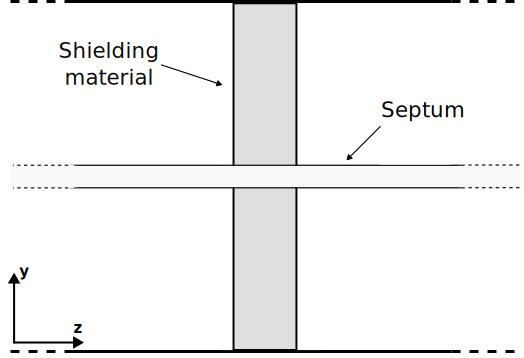
\includegraphics[width=\textwidth]{content/img/ASTM ES7-83.png}
        \caption{Shielding material in TEM cell}
        \label{fig:ASTM ES7-83}
    \end{subfigure}%
    \hfill
    \begin{subfigure}[h]{0.49\textwidth}
        \centering
        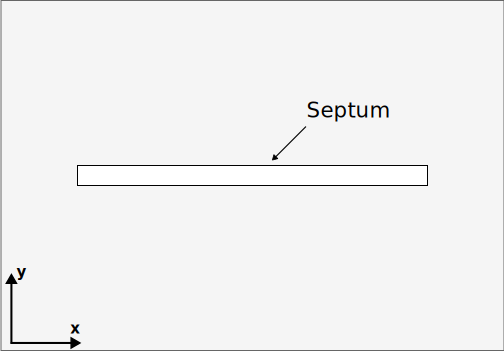
\includegraphics[width=\textwidth]{content/img/form_of_shielding_material.png}
        \caption{Shape of the shielding material}
        \label{fig:form_of_shielding_material}
    \end{subfigure}
    \label{fig:subfigures}
\end{figure}

Then, the S-parameters derived in the simulations are used to get to the output powers $P_\mathrm{ref}$ and $P_\mathrm{load}$. By exciting the TEM cell with a power of 1\,W, the reference power $P_\mathrm{ref}=1\,\mathrm{W}$. The measured power is then derived through

\begin{equation}
    P_\mathrm{load}=P_\mathrm{ref}\cdot10^{|S_\mathrm{12, dB}|/10}.
    \label{eqn:load_power}
\end{equation}

\subsubsection{Dual TEM cell}\label{sec:dual_tem_cell}

The shielding effectiveness of a material may also be determined using a dual TEM cell shown in \autoref{fig:dual_tem_cell}. They are connected through an aperture, which can be filled with the shielding material or left empty. The upper TEM cell is excited through port 1, and acts as a driving cell, transmitting power through the aperture. Port 2 is loaded with the reference impedance $Z_w\approx50\,\Omega$. The second TEM cell functions as a receiver, collecting power at its output ports \cite{MORARI_BĂLAN_2015}.

\begin{figure}[h]
	\centering
	\includegraphics[width=0.75\linewidth]{content/img/dual_tem_cell.png}
	\caption{Dual TEM cell with aperture}
	\label{fig:dual_tem_cell}
\end{figure}

If the aperture is electrically small, its coupling may be described by an electric and a magnetic dipole moment. Their magnitude is related to the electric and magnetic coupling between the TEM cells over the aperture. Therefore, the electric and magnetic coupling can be determined separately by adding or subtracting the output powers of the receiving TEM cell \cite{MORARI_BĂLAN_2015, 4091811}. Consequently, a electric shielding effectiveness $SE_\mathrm{dB}^\mathrm{e}$ and a magnetic shielding effectiveness $SE_\mathrm{dB}^\mathrm{m}$ can be calculated with

\begin{subequations}
	\begin{equation}
		SE_\mathrm{dB}^\mathrm{e}=10\log{\left( \frac{P_\mathrm{ref, sum}}{P_\mathrm{load,sum}} \right)},
		\label{eqn:se_dual_cell_e}
	\end{equation}
	\begin{equation}
		SE_\mathrm{dB}^\mathrm{m}=10\log{\left( \frac{P_\mathrm{ref, diff}}{P_\mathrm{load,diff}} \right)}.
		\label{eqn:se_dual_cell_m}
	\end{equation}
\end{subequations}

Separating the electric and magnetic shielding effectiveness is useful when applying shielding materials in the near field of electric or magnetic dipole moments. For shielding a magnetic dipole moment, the $SE_\mathrm{dB}^\mathrm{m}$ value is considered significant \cite{4091811}, whereas for an electric dipole moment, the $SE_\mathrm{dB}^\mathrm{e}$ value is relevant.

%Because the normalized electric field at the aperture will be of TEM mode, only the component normal to the aperture in z-direction has to be considered. Just as in the case of dipole representation, the Lorentz Reciprocity theorem may be applied to find the fields in the TEM cell. Because both the fields at the output and in the aperture are of TEM mode, only the E-field at the output may be considered. 





\section{Finite Element Method}\label{sec:simulations}
\subsection{Finite Element Method}

\subsubsection{General Idea}
Problems involving the calculations of electromagnetic fields are often cumbersome and difficult to solve. This is due to the need of solving differential equations describing these fields over a computational domain, which is not possible with a computer in this sense. The simulation software Ansys HFSS (High Frequency Simulation Software) aims to provide a solution. This software is used for the simulations in \autoref{sec:simulations}, hence it is described in this following, dedicated section.

HFSS uses a numerical technique, namely the Finite Element Method (FEM). The general idea of FEM after Rayleigh-Ritz-Galerkin is to choose a number of basis functions. The goal is to find a linear combination of these basis functions, so that the differential equation is satisfied as closely as possible. This turns the problem of solving a differential equation into a system of algebraic equations, which the computer can process. There is always a set of basis functions which enable the calculation to converge to the real solution. However, the number of basis functions used in the domain is limited, due to reasons of computability \cite{STRANG_2018}. 

FEM therefore divides the domain into finite elements, i.e. smaller pieces. Then, within each piece, such a basis function is assigned. A linear combination of these basis functions are found, which satisfy the differential equations. In region where the approximating solution has a high degree of error, the accuracy may be increased by further subdividing the finite elements. This is repeated, until the error falls below a certain threshold, and a precise solution is derived.

\subsubsection{Dividing a computational domain into finite elements}

The differential equation to be solved is shown in \autoref{eqn:full_wave_equation}, where $\epsilon_r$ is the relative permeability and $\mu_r$ is the relative permeability of the material. The variable $k_0$ is the wave number of free space and equals $k_0=\omega\sqrt{\epsilon_0\mu_0}$. \cite{Cendes_Lee_1988,85399,Cendes_1991}.

\begin{equation}
    \nabla\times\left(\frac{1}{\mu_r}\nabla\times\mathbf{E}\right)-k_0^2\epsilon_r\mathbf{E}=0 \quad\text{in $\Omega$}
    \label{eqn:full_wave_equation}
\end{equation}

This equation is solved in a computational domain $\Omega$. This computational domain is divided into finite elements, called a mesh. Each node in this mesh has polynomial functions assigned, which are weighted to approximate the real solution. It has been proven that tetrahedral finite elements are best suited for this task, as they are geometrically flexible and make the definition of complete polynomial approximation functions possible \cite{Shenton_Cendes_1985}. Ansys HFSS uses a adaptive finite element mesh generator, which automatically provides a mesh for a given 3-dimensional construction. The Delaunay tesselation for three-dimensions is used for generating a mesh. It efficiently creates a mesh from objects of arbitrary shapes. Any boundary condition can be added recursively to the mesh. At the heart of this algorithm lies the property, that the circumsphere of an tetrahedra's vertices may not contain other tetrahedra's vertices. 

\autoref{fig:tetrahedral_mesh} shows one of such tetrahedrons. At the edge points, the components of the field which are normal to the respective edge and tangential to the face of the element is stored. At the vertex points, the component of a field which are tangential to the edges are stored. The value of the field at any midpoint is derived through interpolation from the node values. The basis function is used for interpolation.

\begin{figure}[h]
    \centering
    \includegraphics[width=0.25\linewidth]{content/img/tetrahedral_mesh.png}
    \caption{Tetrahedron with points on the edge and vertices.}
    \label{fig:tetrahedral_mesh}
\end{figure}

Because of the way how the fields are stored in the tetrahedra, they are called tangetial vector finite elements. Their advantage is that tangential components of fields can be forced to be equal among adjacent tetrahedra at the boundary. For example, an electric field stored at a vertex point must point in the direction along one of the edges, therefore it is tangential to the element. An adjacent element then has the same tangential electric field imposed at this node, leading to a continuous tangential electric field, therefore satisfying the boundary conditions implied by the Maxwell equation automatically. Furthermore, any Dirichlet boundary conditions can easily be set along the edges.
\cite{85399}. 

The finite element is described as \autoref{eqn:finite_element_3d}, where $L_2(\Omega)$ is a set of square integrable functions and $P_1$ a set of piecewise linear functions in the discretized domain $\Omega$ \cite{104986}. The vector fields at the vertices are given as $u$. $D(\Omega)$ is a set of divergence free functions. The vectors $u$ used in the finite element therefore 

\begin{itemize}
    \item are continuous in the normal direction.
    \item are square integrable.
    \item have a curl describable by piecewise linear functions.
\end{itemize}

\begin{equation}
    H^{(\dim=3)}_1(\mathrm{curl}) = \left\{ \mathbf{u} \mid \mathbf{u} \in \left[ L_2(\Omega) \right]^3, \nabla \times \mathbf{u} \in \left[ P_1(\Omega) \right]^3 \cap D(\Omega) \right\}
    \label{eqn:finite_element_3d}
\end{equation}

\autoref{fig:tetrahedra_w_unknowns} shows the finite element with the unknowns marked at each point. For reasons of simplicity, only the face is shown. The variables $u_i^j$ and $u_j^i$ are imposed across element boundaries, therefore guaranteeing tangential continuity at boundaries. Additionally, they inherently defined a linear polynomial, meaning that they describe a gradient of the field along this edge. \autoref{eqn:tangential_vector_component} describes this relation mathematically, where $\mathbf{t}_{ij}$ is the unit vector tangentially to the edge from node i to node j and $l_{ij}$ is the length of this edge.

\begin{equation}
    \mathbf{u}\cdot\mathbf{t}_{ij}=\frac{1}{l_{ij}}\left( u_i^j-u_j^i \right)
    \label{eqn:tangential_vector_component}
\end{equation}

\begin{figure}[h]
    \centering
    \includegraphics[width=0.25\linewidth]{content/img/tetrahedra_w_unknowns.png}
    \caption{Face of the finite element with unknowns}
    \label{fig:tetrahedra_w_unknowns}
\end{figure}

Two facial unknowns $f_1$ and $f_2$ are added to two of the three edge points at one face. Contrary to the variables $u_i^j$, the facial unknowns $f_i$ are only assigned locally at each element and do not cross boundaries. The purpose of the facial unknowns $f$ is to provide a quadratic polynomial for the field component normal to the edges. This will lead to a linear approximation for the curl of the unknown vector field $\nabla\times \mathbf{u}$, providing sufficient accuracy. The overall vector field of this element is then calculated by a superposition of all nodes' vector attributions.

\subsubsection{Solving the differential equation}

A testing function $\mathbf{W}_n$ is defined, which is multiplied to \autoref{eqn:full_wave_equation}. Integrating over the whole test volume then leads to \autoref{eqn:test_funct}. This yields $N$ equations, with $n=1,2,...N$, for each finite element in the domain $\Omega$. This is a common procedure in FEM, and it works through orthogonalization of the residual of \autoref{eqn:full_wave_equation} with respect to the function $\mathbf{W}_n$. This means the new goal of the solution is to minimize the residual by making $\mathbf{W}_n$ as orthogonal as possible \cite{Mohsen_1982}.

\begin{equation}
    \int_\Omega\left( \mathbf{W}_n\cdot\nabla \times\left( \frac{1}{\mu_r}\nabla\times\mathbf{E} \right)-k_0^2\epsilon_r\mathbf{W}_n\cdot\mathbf{E} \right)\mathrm{d}V=0
    \label{eqn:test_funct}
\end{equation}

Using the vector identity $\nabla\cdot\left(\mathbf{a}\times\mathbf{b}\right)=\left(\nabla\times\mathbf{a}\right)\cdot\mathbf{b}-\mathbf{a}\cdot\left(\nabla\times\mathbf{b}\right)$  on \autoref{eqn:test_funct} provides a weak form of the equation, meaning a form of the original partial differential equation, which does not contain all original derivatives \cite{Cendes_Lee_1988,Cendes_1991}. Additionally, boundary terms come into play, as seen in the right hand side of the resulting \autoref{eqn:greens_theorem_wave_eqn}. The usefulness in this step has been described as lowering the highest-order derivative, therefore the approximating functions need to guarantee continuity of value, not of slope \cite{huebner2001finite}. Another explanation is the possibility of incorporation of Neumann boundary conditions \cite{Mohsen_1982}. 

\begin{equation}
    \int_\Omega \left[ \left(\nabla \times \mathbf{W}_n \right)\cdot \frac{1}{\mu_r}\nabla\times \mathbf{E}-k_0^2\epsilon_r\mathbf{W}_n\cdot\mathbf{E}\right]\mathrm{d}V=\underbrace{\oint_{\partial\Omega}\left( \mathbf{W}_n\times \frac{1}{\mu_r}\nabla\times\mathbf{E}\right)\cdot\mathrm{d}\mathbf{S}}_{\text{Boundary term}}
    \label{eqn:greens_theorem_wave_eqn}
\end{equation}

Next, the electric field $\mathbf{E}$ is represented by a superposition of basis functions. When applying Galerkin's method, the basis functions are equal to the test functions $W_n$. \autoref{eqn:representation_e_field_fem} demonstrates the sum of the basis functions, which are weighted with the variable $x_m$. These variables $x$ for all elements have to be solved, to find the electric field $\mathbf{E}$ over the whole domain. The FEM has therefore reduced the initial wave equation in \autoref{eqn:full_wave_equation} to a simple linear matrix equation $Ax=b$, where $A$ is a known $N\times N$ matrix, $b$ contains port excitations and $x$ is the unknown. Ideally, the basis functions are defined to be zero outside of their adjacent elements. This will result to zero for all entries in the matrix, where the test and basis function do not overlap. Therefore, the matrix is sparse, and will be solved much faster. In the end, other electromagnetic quantities can all be derived through the electric field.

\begin{equation}
    \mathbf{E}=\sum^N_mx_m\mathbf{W}_n
    \label{eqn:representation_e_field_fem}
\end{equation}

\autoref{eqn:matrix_a} shows what the matrix then looks like. Some manipulation on the boundary term have been made, so that it contains the surface impedance $Z_s$. The surface impedance defines the ratio of the electric field to the magnetic field on the boundary region. Furthermore, it contains the free space, which equals $\eta_0 \approx 377\,\Omega$.

\begin{equation}
A_{ij} = \int_{\Omega} \nabla \times \mathbf{W}_i \, \frac{1}{\mu_r} \nabla \times \mathbf{W}_j \, \mathrm{d}V 
- k_0^2 \int_{\Omega} \mathbf{W}_i \, \varepsilon_r \mathbf{W}_j \, \mathrm{d}V 
+ \mathrm{i} k_0 \left(\frac{\eta_0}{Z_s}\right) \oint_{\partial\Omega} \mathbf{n} \times \mathbf{W}_i \cdot \mathbf{n} \times \mathbf{W}_j \, \mathrm{d}\mathbf{S}
\label{eqn:matrix_a}
\end{equation}

\subsubsection{Adaptive solution process}

Each finite element therefore has a solved electric field assigned, which should approximate the real solution as closely as possible. To determine the error for each element, \autoref{eqn:full_wave_equation} is evaluated. The elements with the highest residuals contain the largest deviation from the real result, meaning they have a large degree of error. Region in the mesh with large degrees of errors are refined, i.e. the tetrahedral finite elements are split into smaller ones. This allows the FEM solver to recalculate the fields in this region with higher precision, leading to a smaller residual. Consequently, the finite elements represent the fields more accurately, due to a smaller element size and higher resolution \cite{1063929}. An additional method is increasing the order of the polynomial basis functions of elements with low degree of accuracy.

\begin{equation}
    \nabla\times\left(\frac{1}{\mu_r}\nabla\times\mathbf{E}_{\mathrm{solved}}\right)-k_0^2\epsilon_r\mathbf{E}_{\mathrm{solved}}=residual
    \label{eqn:full_wave_equation_solved}
\end{equation}

To determine when the iterative refinement process is done and the solution good enough, some kind of threshold must be defined. One possibility is the $\mathrm{Max}\ \Delta \mathrm{S}$ parameter. It is compared to the difference of S-parameters of the defined excitation ports over two iterations. If, after a mesh refinement, the S-parameters of the ports do not significantly change anymore, meaning change less than $\mathrm{Max}\ \Delta \mathrm{S}$, then the iterative process can be considered done. This described iterative process is shown in \autoref{fig:workflow_fem}. 

\begin{figure}[h]
    \centering
    \includegraphics[width=0.75\linewidth]{content/img/workflow_fem.png}
    \caption{Adaptive solution process}
    \label{fig:workflow_fem}
\end{figure}

\todo{Short HFSS introduction with boundary conditions, ports and modal and terminal solutions?}
 % Fehlende Ressourcen von Zoltan in Journal of Applied Physics. Schreibe über mathetmaische Grundlagen, Meshing, Dipole Excitation und Impedance Network Boundary Counditions (INBC)

% Additional missing ressource: Finite Elements, Electromagnetics, and Design



\input{content/30_numerical_investigations/32_considerations}
\subsection{Monopole Antenna}\label{sec:monopole}
\subsubsection{Setup}
\FloatBarrier

\begin{figure}[htbp]
	\centering
	\hspace*{-0.0cm}
	\begin{subfigure}[t]{0.48\textwidth}
		\centering
		\includegraphics[height=8cm]{content/img/monopole_near_field}
		\caption{Electric near-field intensity}
		\label{fig:monopolenearfield}		
	\end{subfigure}
	\hfill
	\begin{subfigure}[t]{0.48\textwidth}
		
		\centering
		\raisebox{0.1cm}{\includegraphics[height=8cm]{content/img/monopole_antenna}}
		\caption{Geometry of monopole antenna}
		\label{fig:monopoleantenna}
	\end{subfigure}
	
	\caption{The geometrical aspects of the cylindrical monopole antenna, as implemented in the simulation model, with the respective electric near-field plot.}
	\label{fig:field_monopole_antenna}
\end{figure}

The monopole antenna is the simplest antenna capable of generating an electric dipole moment without any accompanying magnetic dipole moment. It is therefore analyzed first, to isolate the mechanisms behind electric dipole radiation from those of other antenna types discussed later in this chapter. As shown in \autoref{fig:monopoleantenna}, it is installed inside the TEM cell and connected to the feed point on the top wall, pointing towards the septum. The current flowing through the antenna is aligned with the electric field of the TEM mode, thereby producing an electric dipole moment according to \eqref{eqn:e_int_a} and \eqref{eqn:e_int_b}, which are further investigated in \cref{sec:eq_dip_mon}.

The antenna has a physical length of 5\,mm, making it electrically short across the entire frequency range of interest (up to 6\,GHz). Below 1.25\,GHz, the antenna is well approximated as an infinitesimal electric dipole, as discussed in \cref{sec:infinitesimal_electric_dipoles}. At higher frequencies, up to 6\,GHz, the finite current distribution along the wire demonstrated in \cref{sec:current_antenna_mon} becomes non-negligible, and the antenna is instead treated as a small electric dipole, as described in \cref{sec:small_electric_dipole}.

Numerically, the near-field distribution exhibits strong displacement currents near the feed point and at the antenna tip. To accurately resolve these localized field concentrations, the mesh element size is reduced in both regions, according to the procedure presented in \cref{sec:mesh}.

Because the electric dipole moment dominates the radiation mechanism, power transfer to the output ports occurs exclusively through displacement current coupling to the septum, as demonstrated in \cref{sec:el_small_antennas}. The induced septum current is analyzed in \cref{sec:sep_curr_mon} for two cases: the propagation of the TEM mode alone, and exclusive propagation of the TE\textsubscript{01} mode.

As an open-circuit structure, the monopole antenna exhibits capacitive behavior. Its effect on the frequency dependence of the feed voltage, current, and input impedance is discussed in \cref{sec:v_c_z_mon}. The output power produced by the antenna is compared against that of the equivalent dipole moments in \cref{sec:output_power_mon} to validate the simulation models.

Lastly, the theoretical framework and numerical results established in this thesis are combined in \cref{sec:monopole_eqc} to construct an equivalent circuit model, which represents the antenna, TEM cell and their coupling components. The circuit model provides an analytical description and deeper understanding of the driving coupling mechanisms between the TEM cell and the monopole antenna.

\subsubsection{Equivalent dipole moments}\label{sec:eq_dip_mon}

The equivalent electric and magnetic dipole moments, $\mathbf{m}_e$ and $\mathbf{m}_m$, are analytically derived using \eqref{eqn:ifa_me} and \eqref{eqn:ifa_mm}. The resulting $\mathbf{m}_e$ shown in \autoref{fig:dipolemomentsmonopolewide} increases approximately linearly over frequency, while the magnetic dipole moment $\mathbf{m}_m$ remains negligible throughout the investigated frequency range. This linear increase directly reflects the linear frequency dependence of the antenna current, as described by \eqref{eqn:e_int_a} and \eqref{eqn:e_int_b}, which relate the electric dipole moment to the antenna current. The frequency dependence of the current itself is shown in \autoref{fig:monopolefeedpointvoltagecurrent} and discussed further in \cref{sec:v_c_z_mon}.

\begin{figure}[htbp]
	\centering
	\includegraphics[width=1\linewidth]{content/img/dipole_moments_monopole_wide}
	\caption{The equivalent electric and magnetic dipole moments analytically calculated with \eqref{eqn:ifa_me} and \eqref{eqn:ifa_mm}. To enable direct comparison with the magnetic dipole moment, the electric dipole moment is weighted with the free space impedance $\eta_0$, as discussed in \cref{sec:prep_dip}.}
	\label{fig:dipolemomentsmonopolewide}
\end{figure}


%\begin{figure}[htbp]
%	\centering
%	\begin{subfigure}[b]{0.48\textwidth}
	%		\centering
	%		\includegraphics[width=1\linewidth]{content/img/dipole_moments_monopole.png}
	%		\caption{Equivalent dipole moments to model the monopole antenna.}
	%		\label{fig:dipole_moments_monopole}
	%	\end{subfigure}
%	\hfill
%	\begin{subfigure}[b]{0.48\textwidth}
	%		\centering
	%		\includegraphics[width=1\linewidth]{content/img/phase_shift_monopole}
	%		\caption{Phase shift of the power between the output ports produced by the monopole antenna.}
	%		\label{fig:phaseshiftmonopole}
	%	\end{subfigure}
%	
%	\caption{The equivalent dipole moments and the corresponding induced phase shift of the power between the output ports delivers information about the electric and magnetic coupling behavior of the monopole antenna.}
%	\label{fig:monopole_moments_phase}
%\end{figure}


\subsubsection{Feed voltage, current and impedance}\label{sec:v_c_z_mon}

The feedpoint voltage $V$ of the antenna, shown in \autoref{fig:monopolefeedpointvoltagecurrent}, remains largely constant over the investigated frequency range. Consequently, the voltage induced between the antenna and the septum is negligible, which is an observation consistent with the absence of a magnetic dipole moment $\mathbf{m}_m$ according to \autoref{eqn:m_v}. 

The feedpoint current $I$, shown in \autoref{fig:monopolefeedpointvoltagecurrent}, increases linearly with frequency. Since the monopole antenna has no return path, the entire current flows as displacement current, partially back toward the feedpoint as a reactive near-field component, and partially toward the septum, as is visible in \autoref{fig:monopolenearfield}. As described by \eqref{eqn:me_i}, $\mathbf{m}_e$ is directly proportional to this displacement current, which explains the observed linear increase of $\mathbf{m}_e$ with frequency. The constant feed voltage over frequency further supports this picture, since a frequency-independent voltage across a capacitive impedance must produce a displacement current that increases linearly with frequency. 

The capacitive nature of the antenna impedance is confirmed by the impedance plot in \autoref{fig:monopoleimp}, which shows a high impedance magnitude at low frequencies that decreases rapidly with increasing frequency. This behavior is characteristic of a capacitive impedance and is consistent with the prediction of \eqref{eqn:compl_power_inf_elec_dipole} and the discussion in \cref{sec:infinitesimal_electric_dipoles}.

\begin{figure}[htbp]
	\centering
	\begin{subfigure}[t]{0.48\textwidth}
		\centering
		\includegraphics[width=1\linewidth]{content/img/monopole_feedpoint_voltage_current}
		\caption{Voltage and current at feedpoint over frequency}
		\label{fig:monopolefeedpointvoltagecurrent}
	\end{subfigure}
	\hfill
	\begin{subfigure}[t]{0.48\textwidth}
		\centering
		\includegraphics[width=1\linewidth]{content/img/monopole_imp}
		\caption{Antenna impedance over frequency}
		\label{fig:monopoleimp}
	\end{subfigure}
	
	\caption{Magnitude of the voltage and current applied at the feedpoint of the monopole antenna over frequency, derived through the S-parameters with \eqref{eqn:iin} and \eqref{eqn:vin}, with the respective magnitude and phase of the antenna impedance over frequency, derived through the S-parameters with \eqref{eqn:za}.}
	\label{fig:monopoleimpvoltcurr}
\end{figure}

%The electric current present in the monopole antenna is aligned with the electric field $\mathbf{e}_\mathrm{TEM}^\pm$ of the dominant TEM mode present in the investigated frequency range. The electric dipole moment in y-direction suffices to model the antenna, because they align with the fields of the TEM mode.

\subsubsection{Current along antenna}\label{sec:current_antenna_mon}

Determining the distribution of the current along the monopole antenna validates the accuracy  of the numerical results and theoretical assumptions made previously. The current is numerically derived by integrating the magnetic field intensity $\mathbf{H}$ along a closed loop $C$ around the wire using Ampère's law,

\begin{equation}
	\oint_C \mathbf{H} \cdot d\mathbf{l'} = I.
	\label{eqn:ampere_law_fem}
\end{equation}

A fine mesh resolution is essential for obtaining accurate results from \eqref{eqn:ampere_law_fem}, as the obtained current values depend directly on the computed near-fields, which are particularly susceptible to numerical inaccuracies, as discussed in \cref{sec:mesh}. A coarse mesh causes non-linear behavior near the feedpoint at $0\,\mathrm{mm}$ in \autoref{fig:monopole_current_dist}, where significant displacement currents and numerical artifacts cause the current distribution to exhibit a steeper decline with non-physical oscillations.

The current distribution at $3\,\mathrm{GHz}$, shown in \autoref{fig:currentdistributionmonopole}, exhibits an approximately linear decrease from the feedpoint to zero at the antenna tip, consistent with the small electric dipole behavior described in \cref{sec:small_electric_dipole}. At $1\,\mathrm{MHz}$, shown in \autoref{fig:currentloopchargedistribution1mhz}, the variation in current along the antenna arm is negligible due to the antenna's small electrical size ($\ll\lambda/ 50$), and the current can be treated as constant, justifying the approximation of the monopole antenna as an infinitesimal electric dipole, as described in \cref{sec:infinitesimal_electric_dipoles}.

The electric dipole moment can be determined by integrating the current distribution along the monopole antenna according to \eqref{eqn:e_int_a} and \eqref{eqn:e_int_b}. At a frequency of 3\,GHz, this approach yields

\begin{equation}
	\mathbf{m}_\mathrm{e}(f=3\,\mathrm{GHz})=\int_{b/2-5\,\mathrm{mm}}^{b/2} I(y, f=3\,\mathrm{GHz})\,dy\, \mathbf{\hat{a}}_y = 85.69\,\upmu\mathrm{Am}\,\mathbf{\hat{a}}_y,
\end{equation}

which corresponds to $\mathbf{m}_e\cdot \eta_0=3.23\cdot 10^{-2} \cdot\,\mathrm{Vm}\,\mathbf{\hat{a}}_y$ when normalized by the free-space wave impedance $\eta_0$. This agrees well with the value of $\mathbf{m}_{e}$ in \autoref{fig:dipolemomentsmonopolewide} at 3\,GHz, therefore supporting the validity of \eqref{eqn:e_int_a} and \eqref{eqn:e_int_b}. 



\begin{figure}[htbp]
	\centering
	\begin{minipage}[t]{0.48\textwidth}
		\centering
		\centering
		\includegraphics[width=1\linewidth]{content/img/monopole_current_dist}
		\caption{Current distribution at $3\,\mathrm{GHz}$}
		\label{fig:currentdistributionmonopole}
		\hfill
	\end{minipage}
	\hfill
	\begin{minipage}[t]{0.48\textwidth}
		\centering
		\includegraphics[width=1\linewidth]{content/img/current_loop_charge_distribution_1MHz}
		\caption{Current distribution at $1\,\mathrm{MHz}$}
		\label{fig:currentloopchargedistribution1mhz}
	\end{minipage}
	\caption{The current distribution along the monopole antenna at $3\,\mathrm{GHz}$ and $1\,\mathrm{MHz}$.}
	\label{fig:monopole_current_dist}
\end{figure}

\FloatBarrier
\subsubsection{Current distribution on septum}\label{sec:sep_curr_mon}
\FloatBarrier

\begin{figure}[htbp]
	\centering
	\begin{subfigure}[b]{1\textwidth}
		\centering
		\includegraphics[width=1\linewidth]{content/img/monopole_surface_currents.png}
		\caption{Current surface density at 3\,GHz, where mostly the TEM mode propagates.}
		\label{fig:monopole_surface_currents}
	\end{subfigure}
	
	\vspace{1em} % Add vertical space between subfigures
	
	\begin{subfigure}[b]{1\textwidth}
		\centering
		\includegraphics[width=1\linewidth]{content/img/monopole_surface_currents_te01.png}
		\caption{Current surface density of only the TE\textsubscript{01}-mode at 3.3\,GHz with the TEM mode compensated.}
		\label{fig:monopole_surface_current_te01}
	\end{subfigure}
	
	\caption{Current surface densities at different frequencies, below and above the cut-off frequency of the TE\textsubscript{01}-mode.}
	\label{fig:surface-current}
\end{figure}

The monopole antenna transfers power to the output ports by inducing a current on the septum. This current is shown in \autoref{fig:monopole_surface_currents} at 3\,GHz. The current arrives at both output ports in phase, confirming the absence of a phase shift between the output port powers. This observation is consistent with the assumption that a pure electric dipole moment introduces no phase shift between the output port powers, as discussed in \cref{sec:equ-dip-mom}.

\autoref{fig:monopole_surface_current_te01} shows the septum surface current density at 3.3\,GHz, with the TEM mode suppressed at the output ports such that only the TE\textsubscript{01} mode propagates. The magnetic field of this mode has a $z$-component that increases gradually towards the cell walls, driving septum currents with an $x$-component that grows in magnitude toward the septum edge. Furthermore, the power induced at the two output ports exhibits a phase shift of $\pi$, a consequence of the TE\textsubscript{01} mode magnetic field being out of phase at the two ports, in contrast to the TEM mode, as explained in \cref{sec:equ-dip-mom}.

\subsubsection{Output power}\label{sec:output_power_mon}

The output power produced by the equivalent dipole moments $\mathbf{m}_e$ and $\mathbf{m}_m$ is compared to that of the monopole antenna in \autoref{fig:monopolemomentcomp}, showing agreement within a $\pm10\,$µW range. This demonstrates that the antenna is effectively represented by its equivalent dipole moments, further supporting the theoretical framework constructed in \cref{sec:el_small_antennas}, which connects electrically small antennas to their produced dipole moments.

The electric field $E^\pm_y$ at $x=0$, $y=b/4$, $z=\pm l/2$, shown in \autoref{fig:monopoleoutputpower}, increases linearly with frequency, consistent with the linearly increasing $\mathbf{m}_e$ magnitude and the resulting quadratic increase in output power. Furthermore, $E^\pm_y$ closely follows the frequency dependence predicted by \eqref{eqn:approx_e_field}, confirming the analytical approximation of the normalized electric field intensity derived in the preliminary theoretical discussion.

\begin{figure}[htbp]
	\centering
	\begin{subfigure}[t]{0.48\textwidth}
		\centering
		\includegraphics[width=1\linewidth]{content/img/monopole_output_power}
		\caption{$E_\mathrm{y}$ and power at output port}
		\label{fig:monopoleoutputpower}
	\end{subfigure}
	\hfill
	\begin{subfigure}[t]{0.48\textwidth}
		\centering
		\includegraphics[width=1\linewidth]{content/img/monopole_moment_comp}
		\caption{Comparison of output powers}
		\label{fig:monopolemomentcomp}
	\end{subfigure}
	\caption{Electric field component $E_\mathrm{y}$ at $x=0$, $y=b/4$, $z=\pm l/2$ and the corresponding output port power, computed from the S-parameters using \eqref{eqn:power_antenna}. The output power of the monopole antenna is compared against that produced by the equivalent dipole moments to validate the model.}
	\label{fig:monopole_power_comp}
\end{figure}

\FloatBarrier
\subsubsection{Equivalent circuit model}\label{sec:monopole_eqc}
\FloatBarrier

Equivalent circuit models of the antenna and the TEM cell are valuable tools 
for further analysis, as they allow the coupling mechanisms to be expressed in terms of measurable lumped circuit parameters. For the monopole antenna, an RLC series circuit for a short electric dipole \cite[p.~8]{Chu_1948} is applied, as demonstrated in \autoref{fig:eqc_simple_monopole}, where $R_A$, $L_A$ and $C_A$ represent the impedance behavior of the antenna.

\begin{figure}[h]
	\centering
	\resizebox{0.35\textwidth}{!}{
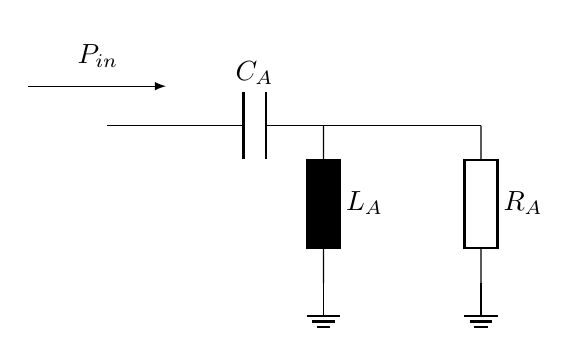
\begin{tikzpicture}
	% Capacitor in series
	\draw (7, 8) to[capacitor, l={$C_A$}] (8.75, 8);
	
	% Top horizontal wire connecting the two parallel branches
	\draw (8.75, 8) -- (10.75, 8);
	
	% Inductor branch (left, vertical) with its own ground
	\draw (8.75, 8) to[european inductor, l={$L_A$}] (8.75, 6);
	\node[ground] at (8.75, 6){};
	
	% Resistor branch (right, vertical) with its own ground
	\draw (10.75, 8) to[european resistor, l={$R_A$}] (10.75, 6);
	\node[ground] at (10.75, 6){};
	
	% Input wire and arrow
	\draw (7, 8) -- (6, 8);
	\draw[-latex] (5, 8.5) -- (6.75, 8.5);
	\node[shape=rectangle, minimum width=2.215cm, minimum height=0.965cm] 
	at (6.534, 8.75){} node[anchor=north west, align=left, 
	text width=1.827cm, inner sep=6pt] at (5.409, 9.25){$P_{in}$};
\end{tikzpicture}
	}
	\caption{Equivalent circuit for a short electric dipole models 
		the monopole antenna's behavior.}
	\label{fig:eqc_simple_monopole}
\end{figure}

Of primary concern for further analysis are $L_A$ and $C_A$, which are determined with the antenna model placed on a PEC surface in free space, as demonstrated in \autoref{fig:free-space-monopole}. The feed current $I_{in}$ is computed according to \eqref{eqn:iin}. The inductance and capacitance are derived according to 
\eqref{eqn:l_m_energy} and \eqref{eqn:c_e_energy}, which leads to 

\begin{subequations}
	\begin{equation}
		L_A = 2\frac{W_m}{I_{in}^2},
	\end{equation}
	\begin{equation}
		C_A = 2\frac{W_c}{V_{CA}^2}= \frac{I_{in}^2}{2\omega^2W_c},
	\end{equation}
\end{subequations}

where $V_{CA}=I_{in}/(j\omega C_A)$ denotes the voltage across the capacitor 
$C_A$. The resulting capacitance equals $C_A=98.36\,\mathrm{fF}$, and the inductance amounts to $L_A=1.14\,\mathrm{nH}$. The resistance $R_A$ generally represents conduction and radiation losses. However, only radiation losses are relevant here, as conduction losses are non-existent due to the use of PECs. The resistance $R_A$ can thereby be derived solely from the effective feed current $I_{in} / \sqrt{2}$ and the radiated power $P_{rad}$ along the radiation boundary, as expressed in 

\begin{equation}
	R_A = \frac{2P_{rad}}{I_{in}^2}.
\end{equation}

The resulting radiation resistance ranges from the milli-ohm range up to $3\,\Omega$ and increases quadratically with frequency.

\begin{figure}[h]
	\centering
	\includegraphics[width=0.7\linewidth]{content/img/free-space-monopole}
	\caption{Model of the monopole antenna connected to a feedpoint mounted 
		on a PEC surface with a side length of $\lambda/2$, where $\lambda$ 
		corresponds to the free-space wavelength of the solution frequency. This 
		configuration enables the investigation of the monopole antenna reactance 
		without influence of the TEM cell.}
	\label{fig:free-space-monopole}
\end{figure}

The antenna equivalent circuit is extended in \autoref{fig:full_circuit_monopole} 
to incorporate the TEM cell's electrical characteristics, represented by a total inductance $L_T = L_{T1} + L_{T2}$ and capacitance 
$C_T = C_{T1} + C_{T2}$, as derived in \cref{sec:tem_cell_model}. The components are split symmetrically ($L_{T1} = L_{T2}$ and $C_{T1} = C_{T2}$) to reflect the physical symmetry of the TEM cell. The source provides a constant input power $P_{in}=1\,\mathrm{W}$ and has a source resistance of $R_s=50\,\Omega$, representing the characteristic impedance of the feedpoint waveport in the simulation model.

The equivalent circuits of the antenna and the TEM cell are coupled via 
$C_k$, which models the displacement current coupling, and the mutual 
inductances $M_{A,T1}$ and $M_{A,T2}$, which account for coupling through 
induced voltages. The mutual inductances are incorporated in the overall schematic through inductor coupling, indicated by the dots next to the inductor symbols. Their relation to the branch voltages and currents is expressed by

\begin{equation}
	\mathbf{V} = j\omega \begin{bmatrix}
		L_{A}     & M_{A,T1} & M_{A,T2} \\
		M_{T1,A}  & L_{T1}   & 0 \\
		M_{T2,A}  & 0        & L_{T2}
	\end{bmatrix} \mathbf{I},
\end{equation}

where $\mathbf{I}=\left[ I_{LA}, I_{LT1}, I_{LT2} \right]^T$ denotes the current vector and $\mathbf{V}=\left[ V_{LA}, V_{LT1}, V_{LT2}  \right]^T$ the voltage vector, and the coupling is assumed to be reciprocal. The coupling elements $C_k$, $M_{A,T1}$, and $M_{A,T2}$ fully represent the power transfer to the TEM cell, rendering a separate radiation resistance $R_A$ redundant.

The key advantage of this approach is the direct derivation of the dipole moments from the circuit: $\mathbf{m}_m$ is obtained from the induced voltages across $L_{T1}$ and $L_{T2}$ in accordance with \eqref{eqn:m_v}, and $\mathbf{m}_e$ from the displacement current through $C_k$ according to \eqref{eqn:me_i}.

\begin{figure}[htbp]
	\centering
	\resizebox{\textwidth}{!}{%
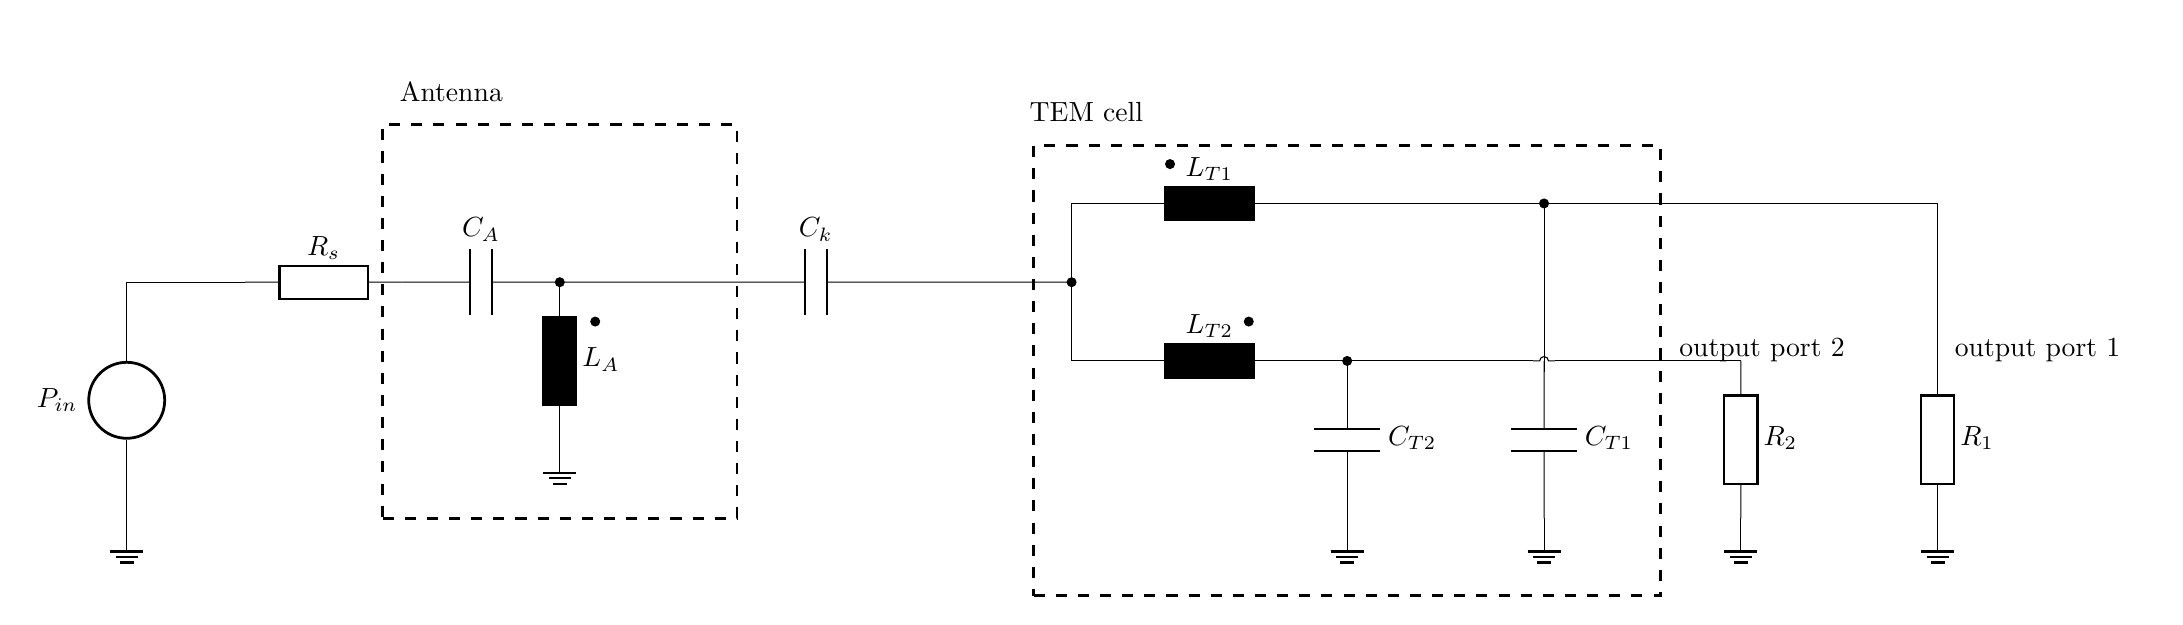
\begin{tikzpicture}
	% Paths, nodes and wires:
	\node[shape=circle, draw, line width=1pt, minimum width=0.965cm]
	(N1) at (2.5, 9.5){} node[anchor=east] at (N1.west){$P_{in}$};
	\node[ground] at (2.5, 8){};
	\draw (2.5, 8) -- (2.5, 9);
	\draw (2.5, 10) -- (2.5, 11) -- (4, 11);
	\draw (4, 11) to[european resistor, l={$R_s$}] (6, 11);
	
	% C_A leads to the junction node
	\draw (6, 11) to[capacitor, l={$C_A$}] (8, 11);
	
	% Junction node where L_A taps off vertically
	\node[circ] at (8, 11){};
	
	% L_A placed vertically to ground (shunt element)
	\draw (8, 11) to[european inductor, l={$L_A$}] (8, 9);
	\node[ground] at (8, 9){};
	
	% Coupling dot on the right side, directly above the L_A label
	\node[circ] at (8.45, 10.5){};
	
	% Horizontal wire continues from junction to C_k
	\draw (8, 11) to[capacitor, l={$C_k$}] (14.5, 11);
	
	\node[shape=rectangle, draw, line width=1pt,
	dash pattern={on 4pt off 4pt}, minimum width=4.5cm,
	minimum height=5cm] at (8, 10.5){};
	\node[shape=rectangle, minimum width=5.215cm, minimum height=1.465cm]
	at (8.375, 13.5){} node[anchor=north west, align=left,
	text width=4.827cm, inner sep=6pt] at (5.75, 13.75){Antenna};
	
	\draw (14.5, 10) to[european inductor, l={$L_{T2}$}] (18, 10);
	\draw (14.5, 12) to[european inductor, l={$L_{T1}$}] (18, 12);
	\draw (14.5, 10) -| (14.5, 12);
	\node[circ] at (14.5, 11){};
	\draw (18, 10) to[capacitor, l={$C_{T2}$}] (18, 8);
	\draw (23, 10) to[european resistor, l={$R_2$}] (23, 8);
	\node[ground] at (18, 8){};
	\node[ground] at (20.5, 8){};
	\node[circ] at (18, 10){};
	\draw (18, 12) -- (22, 12);
	\draw (20.5, 10) to[capacitor, l={$C_{T1}$}] (20.5, 8);
	\node[ground] at (23, 8){};
	\draw (25.5, 10) to[european resistor, l={$R_1$}] (25.5, 8);
	\node[ground] at (25.5, 8){};
	\draw (22, 12) -- (24.5, 12);
	\draw (20.5, 10) -- (20.5, 12);
	\node[jump crossing] at (20.5, 10){};
	\draw (18, 10) -- (20.36, 10);
	\draw (20.64, 10) -- (23, 10);
	\draw (24.5, 12) -| (25.5, 10);
	\node[circ] at (20.5, 12){};
	\node[shape=rectangle, draw, line width=1pt,
	dash pattern={on 4pt off 4pt}, minimum width=7.965cm,
	minimum height=5.715cm] at (18, 9.875){};
	\node[shape=rectangle, minimum width=5.215cm, minimum height=1.465cm]
	at (16.375, 12.75){} node[anchor=north west, align=left,
	text width=4.827cm, inner sep=6pt] at (13.75, 13.5){TEM cell};
	\node[shape=rectangle, minimum width=2.715cm, minimum height=0.965cm]
	at (23.375, 10){} node[anchor=north west, align=left,
	text width=2.327cm, inner sep=6pt] at (22, 10.5){output port 2};
	\node[shape=rectangle, minimum width=2.715cm, minimum height=0.965cm]
	at (26.875, 10){} node[anchor=north west, align=left,
	text width=2.327cm, inner sep=6pt] at (25.5, 10.5){output port 1};
	\node[circ] at (15.75, 12.5){};
	\node[circ] at (16.75, 10.5){};
\end{tikzpicture}
	}
	\caption{Circuit representing the TEM cell and the monopole antenna, with 
		the additional components $C_k$ and $M_{A,T1}$, $M_{A,T2}$ modeling their 
		near-field coupling behavior.}
	\label{fig:full_circuit_monopole}
\end{figure}

The resulting $\mathbf{m}_e$ and $\mathbf{m}_m$ of the monopole antenna are depicted in \autoref{fig:eqc-dipoles-comp} and show quantitative agreement with the dipole moments derived by the simulator.

\begin{figure}[htbp]
	\centering
	\includegraphics[width=1\linewidth]{content/img/eqc-dipoles-comp}
	\caption{Equivalent dipole moments derived by the equivalent circuit compared to the previously derived dipole moments of the monopole antenna, shown in \autoref{fig:dipolemomentsmonopolewide}. The electric dipole moment $\mathbf{m}_e$ is weighted with $\eta_0$ for 
		comparison purposes.}
	\label{fig:eqc-dipoles-comp}
\end{figure}


\FloatBarrier




%\todo[inline]{idea: offset in z-direction, show surface current how it gets a pahse shift at waveports, and a magnetic dipole moment appears to be induced}
%\todo[inline]{idea: offset in x-direction, showing surface current and explaining the decrease in power transfer (normal E-field distribution)}

%If only the TEM mode propagates, only the y-component of an electric dipole moment and the x-component of a magnetic dipole moment generates output power, assuming they are centrally located ($x=0$, $y=b/4$, $z=0$). This is due to the magnetic field containing only an x-component $\mathbf{h}^\pm = h_x^\pm e^{\pm k_0 z}$, and the electric field only an y-component $\mathbf{e}^\pm = e_y^\pm e^{\pm k_0 z}$ at the center of the TEM cell. \todo{Sketch this situation. Also, $e^{\pm k_0 z}$ indicated that at z=0 the dipole moment is located. Consider this in all sketches}
%An offset of dipole moments or propagation of higher order modes lead to different field components of $\mathbf{h}^\pm$ and $\mathbf{e}^\pm$, and therefore to a change in coupling. These effects are investigated numerically in \autoref{sec:dipole_moments}.


\FloatBarrier
%\subsubsection{Electromagnetic energy in the TEM cell}
%\FloatBarrier
%
%The monopole antenna generates electromagnetic fields within the TEM cell, resulting in stored electromagnetic energy. The frequency-dependent electric energy is shown in \autoref{eqn:em_energy}. Its quadratic increase correlates with the output power in \autoref{fig:monopoleoutputpower}. The corresponding magnetic energy is several orders of magnitude smaller due to the capacitive behavior of the monopole antenna and is therefore neglected. From the stored electric energy, both the real and imaginary components of the power consumed by the antenna can be determined.
%
%Moreover, the effective inductance and capacitance of the monopole antenna inside the TEM cell can be derived from the magnetic and electric energy expressions given in \crefrange{eqn:l_m_energy}{eqn:c_e_energy}. Using the peak value of the electric energy shown in \autoref{fig:monopoleelecenergy}, the capacitance is estimated to be $C\approx108.55\,\mathrm{fF}$.
%
%\begin{figure}[htbp]
%	\centering
%	\includegraphics[width=1\linewidth]{content/img/monopole_elec_energy}
%	\caption{Electric energy determined by integrating the electric field over the TEM cell volume, using \autoref{eqn:em_energy}. }
%	\label{fig:monopoleelecenergy}
%\end{figure}

%\begin{figure}[htbp]
%	\centering
%	\begin{subfigure}[b]{0.48\textwidth}
	%	\centering
	%\includegraphics[width=1\linewidth]{content/img/monopole_magn_energy}
	%\caption{Magnetic energy determined with \autoref{eqn:em_energy}}
	%\label{fig:monopolemagenergy}
	%	\end{subfigure}
%	\hfill
%	\begin{subfigure}[b]{0.48\textwidth}
	%	\centering
	%\includegraphics[width=1\linewidth]{content/img/monopole_elec_energy}
	%\caption{Electric energy determined with \autoref{eqn:em_energy}}
	%\label{fig:monopoleelecenergy}
	%	\end{subfigure}
%	
%	\caption{Peak electromagnetic energy in the TEM cell generated by the monopole antenna}
%	\label{fig:monopole_em_energy}
%\end{figure}


\FloatBarrier
\subsection{Loop antenna}\label{sec:loop_sim}
\subsubsection{Setup}

\FloatBarrier

\begin{figure}[tbp]
	\centering
	\raisebox{-4.5mm}{
	\begin{subfigure}[t]{0.49\textwidth}
		\centering
		\includegraphics[width=1\linewidth]{content/img/loop_near_field}
		\caption{Electric near-field intensity of loop antenna}
		\label{fig:loopnearfield}
	\end{subfigure}
}
	\hfill
	\begin{subfigure}[t]{0.48\textwidth}
		\centering
		\includegraphics[width=1\linewidth]{content/img/loop_antenna}
		\caption{Geometry of loop antenna}
		\label{fig:loopantennageometry}
	\end{subfigure}
	
	\caption{The geometry of the loop antenna assimilates a square with round edges. The height and width of the antenna equal $h=w=1.6$\,mm. The return path leads back to the PEC surface of the TEM cell. The electric near-field shows a large displacement current and voltage drop near the feed-point.}
	\label{fig:loopantenna}
\end{figure}

In contrast to the monopole antenna, the loop antenna is the most fundamental antenna capable of generating a magnetic dipole moment and is therefore selected as the second case for further analysis. The geometry of the loop antenna model, positioned inside the TEM cell and connected to a feedpoint on the top cell wall, is shown in \autoref{fig:loopantennageometry}. The antenna consists of three wire segments, each of length $h = w = 1.6\,$mm, and the PEC surface as return path, yielding a total circumference of $C = 6.4\,$mm. The antenna remains electrically short ($C < \lambda/10$) for frequencies up to $4.69\,$GHz. A square loop is preferred over a round geometry in the numerical model, as it enables more accurate mesh generation and cleaner interpretation of the resulting equivalent dipole moments. The mesh is refined on the antenna surface and near the feedpoint, following the preliminary discussion in \cref{sec:mesh}.

The loop antenna is oriented such that the normal vector of its enclosed surface is aligned with the $x$-direction, which maximizes the coupling with the magnetic field component of the TEM mode. Unlike the monopole antenna discussed in \cref{sec:monopole}, the loop antenna provides a current return path. The circulating current induces a rotational electric field, equivalent to a net magnetic field intensity through the loop area, thereby giving rise to a magnetic dipole moment as described by \eqref{eqn:mag_dipole_moment_tem}. Furthermore, displacement currents between the antenna and the septum contribute an electric dipole moment, as expressed in \eqref{eqn:me_i}, analogous to the behavior observed for the monopole antenna. The resulting equivalent electric and magnetic dipole moments are analyzed in detail in \cref{sec:eq_dip_loop}.

The output power produced by the equivalent dipole moments is compared to that radiated by the loop antenna in \cref{sec:output_power_loop}, validating the equivalent dipole models. In \cref{sec:geom_dip_loop}, the influence of the loop antenna geometry is examined by varying its height and width, and analyzing the resulting equivalent dipole moments. This parametric study provides additional insight into how the geometrical properties of the loop antenna influence the equivalent dipole moments.

The electric and magnetic coupling mechanisms between the loop antenna and the TEM cell are directly reflected in the frequency-dependent behavior of the feed voltage, feed current, and antenna impedance. As the relationship between these quantities governs the overall coupling behavior, it is analyzed in \cref{sec:loop_electrical_characteristics}. In addition, the current distribution induced on the septum for varying antenna placements and frequencies is investigated in \cref{sec:current_dist_septum_loop}, with particular attention to the influence of the propagating TEM and TE\textsubscript{01} modes on the coupling behavior.

Following the approach established for the monopole antenna, the theoretical framework and numerical results are combined to derive an equivalent circuit model, presented in \cref{sec:eqc_loop}. This equivalent circuit provides deeper insight into the coupling mechanisms between the antenna and the TEM cell, as well as the interplay between the generated electric and magnetic dipole moments.

\subsubsection{Equivalent dipole moments}\label{sec:eq_dip_loop}

The equivalent dipole moments of the loop antenna are numerically derived by applying \eqref{eqn:ifa_me} and \eqref{eqn:ifa_mm}, and are presented as a function of frequency in \autoref{fig:dipole_moments_loop_antenna}. The phases of the output port powers at ports 1 and 2 are shown in \autoref{fig:loopphase}. Unlike the monopole antenna case, where the phase shift remained zero across the entire investigated frequency range, this phase information is essential for the decomposition of the equivalent dipole moments. A phase shift of zero between the output port powers indicates the presence of an electric dipole moment, whereas a phase shift of $\pm\pi$ is characteristic of a magnetic dipole moment. A phase shift between $0$ and $\pi$ indicates a superposition of both dipole moment contributions, as discussed in detail in \cref{sec:equ-dip-mom}.

The phase shift approaches $\pi$ at low frequencies, indicating that the magnetic dipole moment $\mathbf{m}_m$ dominates over the electric dipole moment $\mathbf{m}_e$. However, the phase shift decreases with frequency, raising the electric dipole moment as a consequence. In contrast to the monopole antenna, $\mathbf{m}_e$ and $\mathbf{m}_m$ thereby demonstrate non-linear behavior over frequency.

\begin{figure}[tbp]
	\centering
	\begin{subfigure}[t]{0.5\textwidth}
		\centering
		\includegraphics[width=1\linewidth]{content/img/dipole_moments_loop_antenna.png}
		\caption{Equivalent dipole moments}
		\label{fig:dipole_moments_loop_antenna}
	\end{subfigure}
	\hfill
	\begin{subfigure}[t]{0.48\textwidth}
		\centering
		\includegraphics[width=1\linewidth]{content/img/loop_phase}
		\caption{Phase of the power at each output port}
		\label{fig:loopphase}
	\end{subfigure}
	
	\caption{Equivalent electric and magnetic dipole moments of the loop antenna as a function of frequency, and the related phase of the power at each output port}
	\label{fig:moments-phase-loop}
\end{figure}

%The surface of the loop equals $S=1.68\,\mathrm{mm}^2$. The magnetic dipole moment $\mathbf{m}_m$ can be approximated by applying \crefrange{eqn:e_a_closed_int}{eqn:m_v}, using the normalized magnetic field intensity of the TEM mode $\mathbf{h}_\mathrm{TEM}^\pm$ and the feed voltage in \autoref{fig:loopfeedreturncurrent}. At 3\,GHz, for example, this yields
%
%\begin{equation}
%	\mathbf{m}_m (f=3\,\mathrm{GHz})=I()\cdot j\omega \mu_0 \frac{S\cdot(\mathbf{h}^-_\mathrm{TEM} - \mathbf{h}^+_\mathrm{TEM})}{2\mathbf{e}^\pm_\mathrm{TEM}\cdot k_0}
%\end{equation}

\subsubsection{Output power}\label{sec:output_power_loop}

The output power and the electric field intensity $E^\pm_y$ at $x=0$, $y=b/4$, $z=\pm l/2$ induced by the loop antenna at the output ports are shown in \autoref{fig:loopopower}. In comparison to the monopole antenna results presented in \autoref{fig:monopoleoutputpower}, both quantities increase more slowly with frequency. This is directly attributed to the concave frequency dependence of the magnetic dipole moment $\mathbf{m}_m$, given that the output power scales quadratically with the dipole moment amplitude. The increase in $\mathbf{m}_e$ does not compensate for this power reduction, as its influence on the output power is small, demonstrated by the analysis in \cref{sec:geom_dip_loop}. The investigation demonstrates that the increasing capacitive coupling at higher frequencies enhances the electric dipole moment contribution and partially opposes the magnetic dipole moment, thereby reducing the overall power transfer.

\autoref{fig:loopopowercomp} demonstrates the output power generated by the equivalent dipole moments $\mathbf{m}_m$, $\mathbf{m}_e$ and the loop antenna. The values agree within $\pm10\,$µW, thereby supporting the validity of the dipole moment model.

\begin{figure}[tbp]
	\centering
	\begin{subfigure}[b]{0.48\textwidth}
		\centering
		\includegraphics[width=1\linewidth]{content/img/loop_opower}
		\caption{Electric field and output power}
		\label{fig:loopopower}
	\end{subfigure}
	\hfill
	\begin{subfigure}[b]{0.5\textwidth}
		\centering
		\includegraphics[width=1\linewidth]{content/img/loop_opower_comp}
		\caption{Comparison of output powers}
		\label{fig:loopopowercomp}
	\end{subfigure}
	
	\caption{Electric field in y-direction $E_\mathrm{y}$ at $x=0, y=b/4, z=\pm l/2$, and the closely related power at one of the output ports, derived with the S-parameters in \autoref{eqn:power_antenna}. The output power produced by the loop antenna is compared with that generated by the equivalent dipole moments.}
	\label{fig:looppowercomparisons}
\end{figure}

\subsubsection{Electric and magnetic energy}

The electric and magnetic energy stored in the TEM cell and produced by the loop antenna are shown in \autoref{fig:loopelectromagneticenergy}, derived by computing \eqref{eqn:em_energy} over the TEM cell volume. At low frequencies, the loop antenna predominantly generates magnetic energy, consistent with its dominant magnetic dipole moment. However, with increasing frequency, the electric energy stored in the TEM cell grows rapidly, associated with increasing electric field intensities. This behavior can be directly connected to the increasing electric dipole moment of the loop antenna, which is driven by the growing displacement currents associated with the rising electric field intensity between the antenna and the septum.

\begin{figure}[htbp]
	\centering
	\includegraphics[width=1\linewidth]{content/img/loop_electromagnetic_energy}
	\caption{Electric and magnetic energy stored in the TEM cell as a function of frequency, produced by the loop antenna.}
	\label{fig:loopelectromagneticenergy}
\end{figure}

\subsubsection{Influence of geometry on dipole moments}\label{sec:geom_dip_loop}

The influence of the antenna geometry on the coupling behavior is investigated to explain the role of geometrical parameters in determining the equivalent dipole moments. The height $h$ and width $w$ of the loop antenna are systematically varied, and the resulting dipole moments and input power consumption are compared.

\begin{figure}[htbp]
	\centering
	\begin{subfigure}[t]{0.5\textwidth}
		\centering
		\includegraphics[width=1\linewidth]{content/img/loop-geomg-comp}
		\caption{Equivalent dipole moments}
		\label{fig:loop-geomg-comp}
	\end{subfigure}
	\hfill
	\begin{subfigure}[t]{0.48\textwidth}
		\centering
		\includegraphics[width=1\linewidth]{content/img/loop-geom-power}
		\caption{Output power}
		\label{fig:loop-geom-power}
	\end{subfigure}
	
	\caption{Equivalent dipole moments and output power for two loop antenna configurations: $h=2.16\,\mathrm{mm},\, w=1.4\,\mathrm{mm}$ and $h=1.2\,\mathrm{mm},\, w=2.36\,\mathrm{mm}$. The electric dipole moment $\mathbf{m}_e$ is weighted by $\eta_0$ to enable direct comparison with $\mathbf{m}_m$.}
	\label{fig:loop-geom-sweep}
\end{figure}

Both configurations share an identical loop area, and consequently exhibit the same magnetic dipole moment $\mathbf{m}_m$, in agreement with \eqref{eqn:e_a_closed_int} and \eqref{eqn:e_b_closed_int}. The nonlinear frequency dependence of $\mathbf{m}_m$ persists across both configurations. In contrast, the electric dipole moment $\mathbf{m}_e$ exhibits a strong dependence on the antenna height $h$. As depicted in \autoref{fig:loop-geomg-comp}, the configuration with $h = 2.16\,\mathrm{mm}$ generates an electric dipole moment more than twice that of the configuration with $h = 1.2\,\mathrm{mm}$, which is a direct consequence of the increased displacement currents arising from the reduced distance between the antenna and the septum. This result is consistent with \eqref{eqn:me_i}, which relates the displacement current between the antenna conductor and the septum to $\mathbf{m}_e$.

Finally, as shown in \autoref{fig:loop-geom-power}, the configuration producing the larger electric dipole moment also yields a slightly higher output power, although the difference remains small. This demonstrates the comparatively limited influence of $\mathbf{m}_e$ on the output power relative to $\mathbf{m}_m$. 


\subsubsection{Feed voltage, current and impedance}\label{sec:loop_electrical_characteristics}


\begin{figure}[tbp]
	\centering
	\begin{subfigure}[t]{0.45\textwidth}
		\centering
		\includegraphics[width=1\linewidth]{content/img/loop_feed_return_current_voltage}
		\caption{Voltage and current}
		\label{fig:loopfeedreturncurrent}
	\end{subfigure}
	\hfill
	\begin{subfigure}[t]{0.45\textwidth}
		\centering
		\includegraphics[width=1\linewidth]{content/img/curr_imp}
		\caption{Impedance}
		\label{fig:currimp}
	\end{subfigure}
	
	\caption{Voltage, current and impedance characteristics of the loop antenna.}
	\label{fig:curr_volt_imp}
\end{figure}

%The difference between the current near the feedpoint and that on the return path increases with frequency, indicating a growing occurrence of displacement currents.  The voltage across the feedpoint is obtained using \autoref{eqn:vin}. Magnitude and phase of the impedance of the loop antenna are determined with \autoref{eqn:za}. \autoref{eqn:vin}

The current $I$ in the loop antenna is evaluated at a distance of $0.17\,$mm above the feedpoint and at the same height above the PEC plane along the return path, as indicated in \autoref{fig:loopantennageometry}. This offset from the feedpoint and the PEC plane reduces numerical artifacts arising from the large displacement currents in their vicinity, thereby improving the accuracy of the extracted current values. The current $I$ is obtained by integrating the magnetic field intensity $\mathbf{H}$ along a closed loop of radius $0.11\,$mm around the respective wire segments, according to \eqref{eqn:ampere_law_fem}. 

The extracted current values differ between the two paths, which indicates that displacement currents couple from the antenna to the septum, giving rise to the electric dipole moment $\mathbf{m}_e$ according to \eqref{eqn:me_i}, and return to the feedpoint, constituting the reactive electric energy stored by the antenna. Furthermore, this difference increases with frequency, consistent with the growing displacement currents and the associated increase in $\mathbf{m}_e$. This observation is in good agreement with $\mathbf{m}_e$ presented in \autoref{fig:dipole_moments_loop_antenna}.

\autoref{fig:loopfeedreturncurrent} demonstrates the voltage at the feedpoint of the antenna. This voltage partly couples with the septum, giving raise to $\mathbf{m}_m$ according to \eqref{eqn:m_v}, and partly constitutes the magnetic energy stored by the antenna. The feed voltage significantly rises with frequency and flattens at higher frequencies, which strongly correlates with the frequency-behavior of $\mathbf{m}_m$. This correlation validates the theoretical framework established describing the magnetic dipole moment creation of antennas in this thesis.

On a side note, the increase in voltage also correlates with the displacement current. It raises the potential on the loop antenna, therefore increasing the charge distributions and displacement currents.

Lastly, the increases in voltage and decrease in current agrees with the impedance, depicted in \autoref{fig:currimp}. The loop antenna also shows strongly inductive behavior, as expected by the pre-dominantly magnetic energy stored, magnetic dipole moment and inductive geometry. 

The feed voltage of the loop antenna is presented in \autoref{fig:loopfeedreturncurrent}. A portion of this voltage couples to the septum, giving rise to the magnetic dipole moment $\mathbf{m}_m$ according to \eqref{eqn:m_v}, while the remainder constitutes the magnetic energy stored in the antenna. The feed voltage increases significantly with frequency before flattening at higher frequencies, a behavior that is reflected in the frequency-dependent behavior of $\mathbf{m}_m$. 

It is further noted that the increasing voltage mirrors an increased potential and charge accumulation on the loop antenna, thereby increasing the displacement currents coupling to the septum. Therefore, the generation of a magnetic dipole moment $\mathbf{m}_m$ in the loop antenna is naturally accompanied by a electric dipole moment $\mathbf{m}_e$. Lastly, the increase in feed voltage and decrease in feed current are consistent with the antenna input impedance shown in \autoref{fig:currimp}. Furthermore, it exhibits strongly inductive behavior, as expected given the predominantly magnetic energy storage, the dominant magnetic dipole moment, and the inherently inductive geometry of the loop antenna.

\subsubsection{Current distribution on septum}\label{sec:current_dist_septum_loop}

The radiating loop antenna induces surface currents on the septum of the TEM cell, as shown in \autoref{fig:loop_surface_current}. At a frequency of 3\,GHz, the currents reaching the output ports are out of phase, as illustrated in \autoref{fig:current_loop_surface_current}. This observation is consistent with the analysis in \cref{sec:equ-dip-mom}, which predicts a phase shift of $\pm\pi$ between the output port powers in the presence of a magnetic dipole moment.

\begin{figure}[htbp]
	\centering
	\begin{subfigure}[b]{1\textwidth}
		\centering
		\includegraphics[width=1\linewidth]{content/img/loop_surface_currents.png}
		\caption{The centrally located loop antenna without offset or rotation at a frequency of 3\,GHz, where mainly the TEM mode propagates.}
		\label{fig:current_loop_surface_current}
	\end{subfigure}
	
	\vspace{1em} % Add vertical space between subfigures
	
	\begin{subfigure}[b]{1\textwidth}
		\centering
		\includegraphics[width=1\linewidth]{content/img/loop_surface_currents_offset_rotation_100MHz}
		\caption{Loop antenna with offset of $x=7\,\mathrm{mm}$ and a $\pi/4$ rotation angle at 100\,MHz, where only the TEM mode propagates. The currents passing to the output ports are negligible.}
		\label{fig:loopsurfacecurrentsoffsetrotation}
	\end{subfigure}
	
	\vspace{1em} % Add vertical space between subfigures
	
	\begin{subfigure}[b]{1\textwidth}
		\centering
		\includegraphics[width=1\linewidth]{content/img/loop_surface_currents_offset_rotation_3GHz3}
		\caption{Loop antenna with offset of $x=7\,\mathrm{mm}$ and a $\pi/4$ rotation angle at 3.3\,GHz, where the TEM and TE\textsubscript{01} modes both propagate. The currents passing to the output ports produce significant power, as shown in \autoref{fig:loopsurfacecurrentsoffsetrotation3ghz3plot}.}
		\label{fig:loopsurfacecurrentsoffsetrotation3ghz3}
	\end{subfigure}
	
	\caption{Surface current density on the septum induced by the loop antenna for different frequencies and positions of the antenna.}
	\label{fig:loop_surface_current}
\end{figure}

\begin{figure}[htbp]
	\centering
	\includegraphics[width=1\linewidth]{content/img/loop_surface_currents_offset_rotation_3GHz3_plot}
	\caption{Output power transmitted by the antenna to the output port through the TEM and TE\textsubscript{01} modes, separately over frequency, determined through the S-parameters with \autoref{eqn:power_antenna}. At a frequency of $f=3.21\,\mathrm{GHz}$ a resonance in the TEM cell occurs, leading to the visible peak in the output power produced by the TE\textsubscript{01} mode. }
	\label{fig:loopsurfacecurrentsoffsetrotation3ghz3plot}
\end{figure}

When the antenna is rotated by $\pm\pi/4$ and offset by $x=7\,\mathrm{mm}$, power transmission at 3\,GHz is insignificant. According to \crefrange{eqn:e_a_closed_int}{eqn:e_b_closed_int} and \autoref{eqn:m_v}, efficient coupling requires the magnetic field intensity of the propagating TEM mode $\mathbf{h}_\mathrm{TEM}^\pm$ to be aligned with the vector normal to the antenna surface. The current distribution \autoref{fig:loopsurfacecurrentsoffsetrotation} demonstrates no excited waves in this configuration. Instead, the power produced by the surface current remains reactive, forming closed circulation patterns around the induced magnetic fields. 

At a frequency of 3.3\,GHz, the TE\textsubscript{01} mode propagates in the TEM cell. In this case, $\mathbf{h}_\mathrm{TE01}^\pm$ aligns with the normal vector of the offset and rotated loop antenna surface. As shown in \autoref{fig:loopsurfacecurrentsoffsetrotation3ghz3}, a significant proportion of the current now reaches the output ports, resulting in transmission of power. In contrast to the previous case, the output powers are in-phase, as discussed in \cref{sec:equ-dip-mom}. The output power transmitted by the TE\textsubscript{01} mode increases sharply with frequency, as demonstrated in \autoref{fig:loopsurfacecurrentsoffsetrotation3ghz3plot}.



\subsubsection{Equivalent circuit model}\label{sec:eqc_loop}

Following the same approach established in \cref{sec:monopole_eqc}, an 
equivalent circuit is derived for the small loop antenna. 
\autoref{fig:eqc_balanis} demonstrates the full equivalent circuit for the 
electrically small loop antenna in free space \cite[p. 244]{Balanis_1997}, 
where

\hspace{1cm}\begin{minipage}{\dimexpr\textwidth-2cm}
	\begin{description}
		\item[$C_s$]   Stray capacitance of the loop antenna
		\item[$R_L$]   Ohmic loss resistance of the antenna conductor
		\item[$R_r$]   Radiation resistance of the loop antenna
		\item[$L_i$]   Internal inductance of the loop antenna
		\item[$L_e$]   External inductance of the loop antenna
	\end{description}
\end{minipage}

As discussed in \cref{sec:antenna_model}, the antenna is modeled as a perfect 
electric conductor, therefore $R_L$ and $L_e$ are neglected. Instead, the 
simplified equivalent circuit in \autoref{fig:eqc_simple} is applied, where 
$R_A$, $L_A$ and $C_A$ represent the impedance behavior of the antenna.

\begin{figure}[tbp]
	\centering
	\begin{subfigure}[b]{0.45\textwidth}
		\centering
		\resizebox{0.7\textwidth}{!}{
			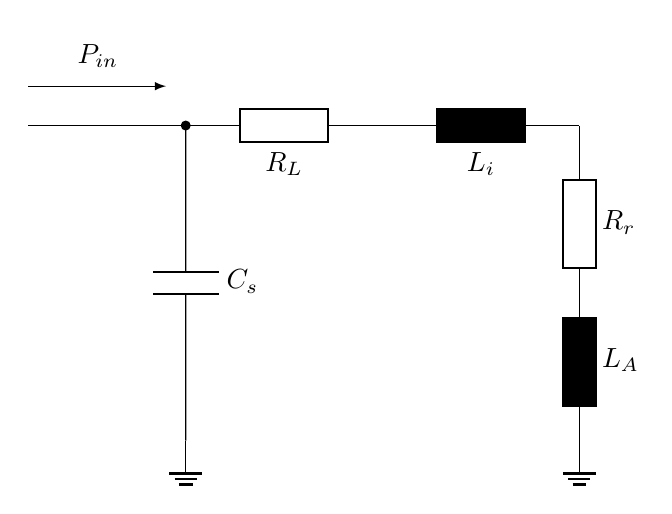
\begin{tikzpicture}
				% Paths, nodes and wires:
				\draw (11.75, 6) to[european inductor, l={$L_{i}$}] (9.75, 6);
				\draw (12, 2) to[european inductor, l_={$L_{A}$}] (12, 4);
				\draw (7, 6) to[capacitor, l={$C_s$}] (7, 2);
				\draw (12, 5.75) to[european resistor, l={$R_{r}$}] (12, 3.75);
				\draw (9.25, 6) to[european resistor, l={$R_{L}$}] (7.25, 6);
				\node[ground] at (7, 2){};
				\node[ground] at (12, 2){};
				\draw (7, 6) -- (5, 6);
				\node[circ] at (7, 6){};
				\draw (7, 6) -- (7.25, 6);
				\draw (9.25, 6) -- (10, 6);
				\draw (11.75, 6) -- (12, 6);
				\draw (12, 5.75) -| (12, 6);
				\draw[-latex] (5, 6.5) -- (6.75, 6.5);
				\node[shape=rectangle, minimum width=2.215cm, 
				minimum height=0.965cm] at (6.534, 6.75){} 
				node[anchor=north west, align=left, text width=1.827cm, 
				inner sep=6pt] at (5.409, 7.25){$P_{in}$};
			\end{tikzpicture}
		}
		\caption{Full equivalent circuit \cite[p. 244]{Balanis_1997}}
		\label{fig:eqc_balanis}
	\end{subfigure}
	\hfill
	\hspace*{-0.5cm}
	\begin{subfigure}[b]{0.45\textwidth}
		\centering
		\resizebox{0.65\textwidth}{!}{
			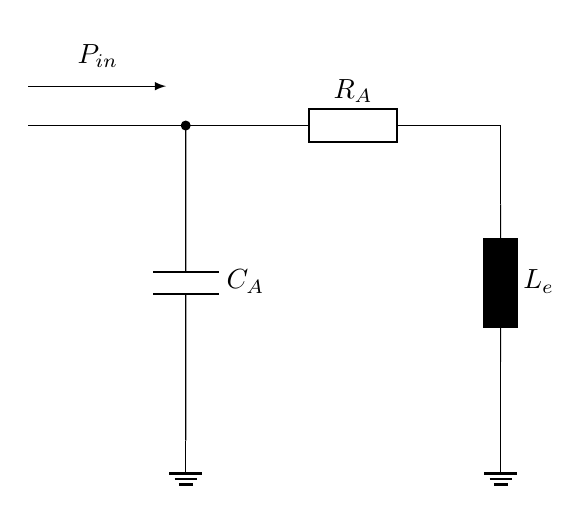
\begin{tikzpicture}
				% Paths, nodes and wires:
				\draw (11, 3) to[european inductor, l_={$L_{e}$}] (11, 5);
				\draw (7, 6) to[capacitor, l={$C_A$}] (7, 2);
				\node[ground] at (7, 2){};
				\node[ground] at (11, 2){};
				\draw (7, 6) -- (5, 6);
				\node[circ] at (7, 6){};
				\draw (7, 6) -- (7.25, 6);
				\draw[-latex] (5, 6.5) -- (6.75, 6.5);
				\node[shape=rectangle, minimum width=2.215cm, 
				minimum height=0.965cm] at (6.534, 6.75){} 
				node[anchor=north west, align=left, text width=1.827cm, 
				inner sep=6pt] at (5.409, 7.25){$P_{in}$};
				\draw (11, 2) -| (11, 3);
				\draw (7.25, 6) to[european resistor, l={$R_A$}] (11, 6);
				\draw (11, 6) -- (11, 5);
			\end{tikzpicture}
		}
		\caption{Reduced equivalent circuit}
		\label{fig:eqc_simple}
	\end{subfigure}
	\caption{Equivalent circuits of the small loop antenna.}
	\label{fig:eqc_loop}
\end{figure}

%The equivalent circuit of the loop antenna can be used to reason about 
%the coupling behavior of the antenna. In particular when assuming that a significant induced voltage $V_n$ occurs across the inductor through magnetic near-field coupling. This voltage $V_n$ is then related to an induced displacement current $I_n$ through the capacitance by
%
%\begin{equation}
%	\frac{I_n}{V_n}=\frac{j\omega Q}{R_A\omega_0^2+j\omega L\omega_0^2
%		-R_w\omega^2},
%	\label{eqn:loop_w0}
%\end{equation}
%
%where $\omega_0 = 1/\sqrt{L_AC_A}$ denotes the resonance frequency, 
%$Q=\omega_0R_wC_A$ the Q-factor of the equivalent circuit and $R_w$ the  characteristic impedance of the antenna feedpoint, assuming that it is purely resistive. Since $V_n$ and 
%$I_n$ are directly associated with the magnetic and electric dipole moments 
%$\mathbf{m}_m$ and $\mathbf{m}_e$ through \cref{eqn:m_v,eqn:me_i}, 
%the electric and magnetic coupling behavior of the small loop antenna can 
%be directly linked to its resonance frequency and Q-factor.
%
%A lower resonance frequency $\omega_0$, higher Q-factor $Q$ or capacitance 
%$C_A$ results in a more pronounced non-linear frequency-behavior of 
%$\mathbf{m}_m$ and $\mathbf{m}_e$. Furthermore, increased capacitance lowers 
%the resonance frequency $\omega_0$ toward the investigated frequency range 
%and increases the antenna's electrical length \cite{Propagation_2022}, both 
%attributing to increased radiated power.

To determine $R_A$, $L_A$ and $C_A$, the antenna model is placed on a PEC 
surface in an open space, as demonstrated in \autoref{fig:free-space-loop}. 
The inductance and capacitance are derived according to 
\crefrange{eqn:l_m_energy}{eqn:c_e_energy}, which leads to

\begin{subequations}
	\begin{equation}
		L_A = 2\frac{W_m}{I_{LA}^2} = \frac{V_{in}^2}{2\omega^2W_m},
	\end{equation}
	\begin{equation}
		C_A = 2\frac{W_c}{V_{in}^2},
	\end{equation}
\end{subequations}

where $I_{LA}=V_{in}/(j\omega L_A)$ denotes the current through the inductor 
$L_A$. The resulting capacitance and inductance equal $C_A=38.2\,\mathrm{fF}$ 
and $L_A=2.14\,\mathrm{nH}$. 

\begin{figure}[tbp]
	\centering
	\includegraphics[width=0.7\linewidth]{content/img/free-space-loop}
	\caption{Model of the loop antenna connected to a feedpoint mounted on a 
		PEC surface with a side length of $\lambda/2$, where $\lambda$ corresponds 
		to the free-space wavelength of the solution frequency. This configuration 
		enables the investigation of the loop antenna reactance without influence 
		of the TEM cell.}
	\label{fig:free-space-loop}
\end{figure}

%The resulting $L_A$ is compared with
%
%\begin{equation}
%	L_\mathrm{sq} = \frac{2\mu_0 l}{\pi} \left[ \ln\!\left(\frac{l}{w_r}
%	\right) - 0.774 \right],
%	\label{eqn:ind_approx}
%\end{equation}
%
%which provides an approximation for the inductance of a square loop antenna 
%in free space \cite[p.~245]{Balanis_1997}. In this expression, $l$ denotes 
%the length of one side of the loop antenna and $w_r$ the wire radius. For 
%the loop antenna under investigation, \autoref{eqn:ind_approx} yields 
%$L_\mathrm{sq}=2.32\,\mathrm{nH}$, which is comparable to the previously 
%obtained $L_A$.
%
%\todo[inline]{Check: Does this formula consider external inductances?}

The antenna equivalent circuit is extended with the TEM cell coupling model 
introduced in \cref{sec:tem_cell_model}, as shown in \autoref{fig:full_circuit_loop}. The coupling components $C_k$, $M_{A,T1}$ and $M_{A,T2}$ are defined analogously to \cref{sec:monopole_eqc}.

\begin{figure}[htbp]
	\centering
	\resizebox{\textwidth}{!}{%
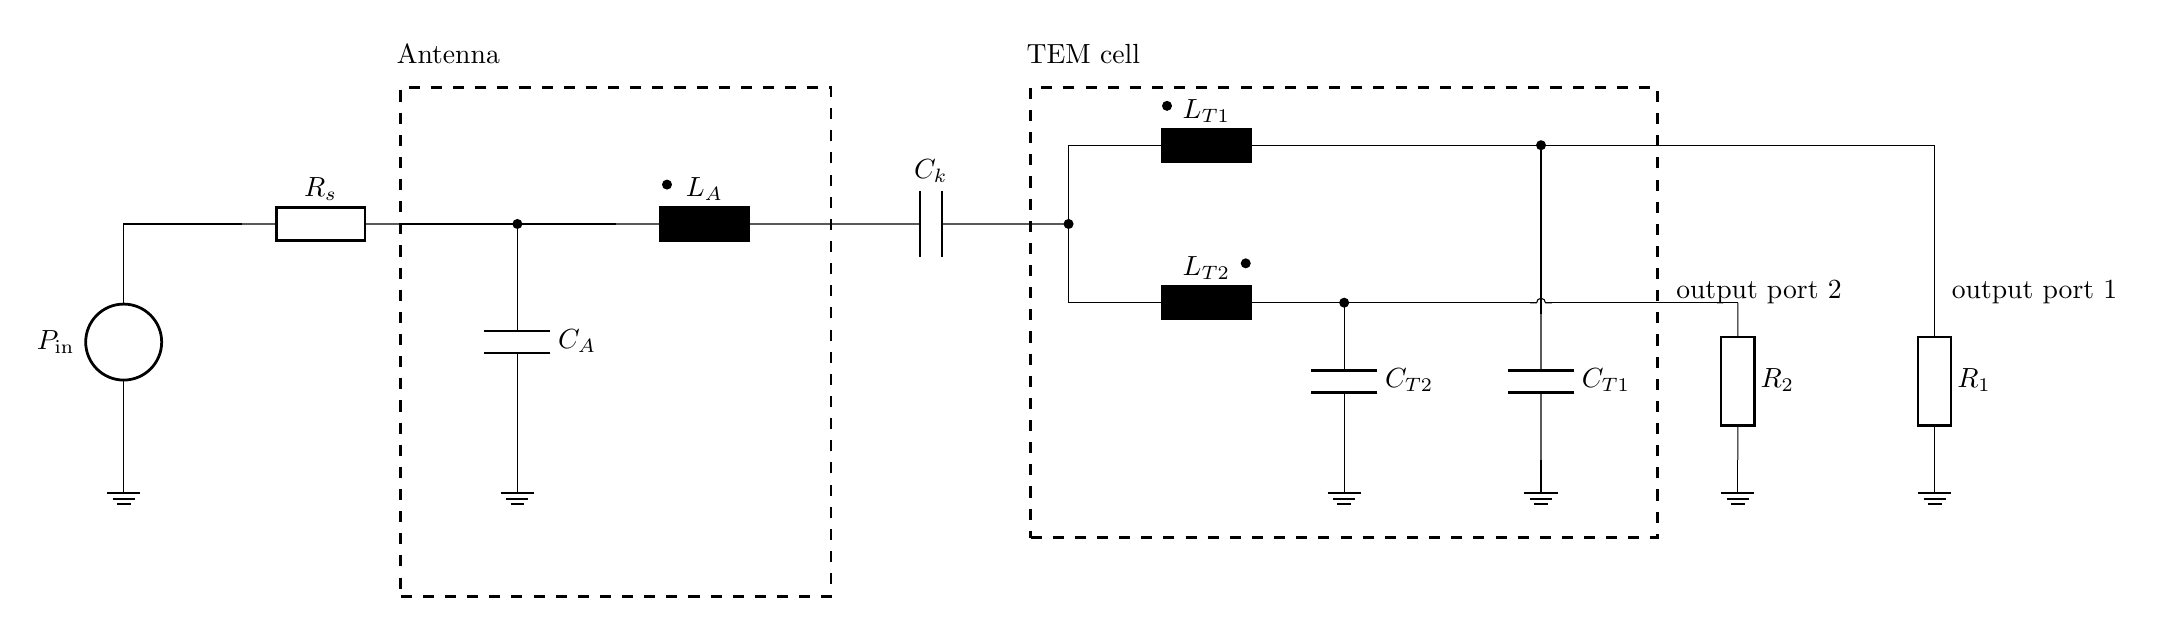
\begin{tikzpicture}
	% Paths, nodes and wires:
	\node[shape=circle, draw, line width=1pt, minimum width=0.965cm]
	(N1) at (2.5, 9.5){} node[anchor=east] at (N1.west){$P_\mathrm{in}$};
	\node[ground] at (2.5, 8){};
	\draw (2.5, 9) -| (2.5, 8);
	\draw (4, 11) to[european resistor, l={$R_s$}] (6, 11);
	\draw (7.5, 11) to[capacitor, l={$C_A$}] (7.5, 8);
	\node[ground] at (7.5, 8){};
	\draw (2.5, 10) -| (2.5, 11) -- (4, 11);
	\draw (6, 11) -- (7.5, 11) -- (8.75, 11);
	\node[circ] at (7.5, 11){};
	\node[circ] at (9.4, 11.5){};
	\node[shape=rectangle, draw, line width=1pt, 
	dash pattern={on 4pt off 4pt}, minimum width=5.465cm, 
	minimum height=6.465cm] at (8.75, 9.5){};
	\node[shape=rectangle, minimum width=5.215cm, minimum height=1.465cm] 
	at (8.375, 11.5){} node[anchor=north west, align=left, 
	text width=4.827cm, inner sep=6pt] at (5.75, 13.5){Antenna};
	\draw (8.75, 11) to[european inductor, l={$L_A$}] (11, 11)
	to[capacitor, l={$C_k$}] (14.5, 11);
	\draw (14.5, 10) to[european inductor, l={$L_{T2}$}] (18, 10);
	\draw (14.5, 12) to[european inductor, l={$L_{T1}$}] (18, 12);
	\draw (14.5, 10) -| (14.5, 12);
	\node[circ] at (14.5, 11){};
	\draw (18, 10) to[capacitor, l={$C_{T2}$}] (18, 8);
	\draw (23, 10) to[european resistor, l={$R_2$}] (23, 8);
	\node[ground] at (18, 8){};
	\node[ground] at (20.5, 8){};
	\node[circ] at (18, 10){};
	\draw (18, 12) -- (22, 12);
	\draw (20.5, 10) to[capacitor, l={$C_{T1}$}] (20.5, 8);
	\node[ground] at (23, 8){};
	\draw (25.5, 10) to[european resistor, l={$R_1$}] (25.5, 8);
	\node[ground] at (25.5, 8){};
	\draw (22, 12) -- (24.5, 12);
	\draw (20.5, 10) -- (20.5, 12);
	\node[jump crossing] at (20.5, 10){};
	\draw (18, 10) -- (20.36, 10);
	\draw (20.64, 10) -- (23, 10);
	\draw (24.5, 12) -| (25.5, 10);
	\node[circ] at (20.5, 12){};
	\node[shape=rectangle, draw, line width=1pt, 
	dash pattern={on 4pt off 4pt}, minimum width=7.965cm, 
	minimum height=5.715cm] at (18, 9.875){};
	\node[shape=rectangle, minimum width=5.215cm, minimum height=1.465cm] 
	at (16.375, 12.75){} node[anchor=north west, align=left, 
	text width=4.827cm, inner sep=6pt] at (13.75, 13.5){TEM cell};
	\node[shape=rectangle, minimum width=2.715cm, minimum height=0.965cm] 
	at (23.375, 10){} node[anchor=north west, align=left, 
	text width=2.327cm, inner sep=6pt] at (22, 10.5){output port 2};
	\node[shape=rectangle, minimum width=2.715cm, minimum height=0.965cm] 
	at (26.875, 10){} node[anchor=north west, align=left, 
	text width=2.327cm, inner sep=6pt] at (25.5, 10.5){output port 1};
	\node[circ] at (15.75, 12.5){};
	\node[circ] at (16.75, 10.5){};
\end{tikzpicture}
	}
	\caption{Circuit representing the TEM cell and the loop antenna, with the 
		additional components $C_k$ and $M_{A,T1}$, $M_{A,T2}$ modeling their 
		near-field coupling behavior.}
	\label{fig:full_circuit_loop}
\end{figure}

The resulting $\mathbf{m}_e$ and $\mathbf{m}_m$ are depicted in 
\autoref{fig:loopeqcmoments}, which are similar to the dipole moments 
derived by the simulator in the higher end of the frequency range. However, accuracy recedes in the low-frequency range.

\begin{figure}[htbp]
	\centering
	\includegraphics[width=1\linewidth]{content/img/loop_eqc_moments}
	\caption{Equivalent dipole moments derived by the equivalent circuit 
		depicted in \autoref{fig:full_circuit_loop}, compared to the dipole moments 
		of the loop antenna, shown in \autoref{fig:dipole_moments_loop_antenna}. 
		The electric dipole moment $\mathbf{m}_e$ is weighted with $\eta_0$ for 
		comparison purposes.}
	\label{fig:loopeqcmoments}
\end{figure}




%\autoref{fig:currentloopchargedistribution} shows the charge density distribution in the current loop antenna. Charges collect, among other locations, at the bottom wire. This leads to electric coupling with the septum. 
%
%\begin{figure}[htbp]
%	\centering
%	\begin{minipage}[b]{0.45\textwidth}
	%		\centering
	%		\includegraphics[width=0.5\linewidth]{content/img/current_loop_charge_distribution}
	%		\caption{Charge density distribution in current loop antenna}
	%		\label{fig:currentloopchargedistribution}
	%	\end{minipage}
%	\hfill
%	\begin{minipage}[b]{0.45\textwidth}
	%		\centering
	%		\includegraphics[width=0.5\linewidth]{content/img/current_loop_current_distribution}
	%		\caption{Current density distribution in current loop antenna}
	%		\label{fig:currentloopcurrentdistribution}
	%	\end{minipage}
%\end{figure}


%The current and voltage drops along the wire are not constant. From the feedpoint to the first corner, there is a much larger voltage drop and current, than from the second corner to the ground plane. Consequently, the power consumed by the first part is much higher than by the latter \todo{Insert power consumption plots of each antenna section}. Additionally, this difference in power consumption increases slightly over frequency. 

%The electric current reduces over the wire because of the displacement current to the septum and the ground plane. As visible in the charge density plot in \autoref{fig:currentloopcurrentdistribution} and the electric field plot in \autoref{fig:currentloopnearefield}, much of the displacement current occurs near the feedpoint and at the wire parallel to the septum. Consequently, this is where the current drops by the most amount. \todo{Insert current distribution plots}



%\begin{figure}[htbp]
%	\centering
%	\begin{minipage}[b]{0.45\textwidth}
	%		\centering
	%		\includegraphics[width=0.7\linewidth]{content/img/current_loop_near_e_field}
	%		\caption{Electric near field in current loop antenna}
	%		\label{fig:currentloopnearefield}
	%	\end{minipage}
%	\hfill
%	\begin{minipage}[b]{0.45\textwidth}
	%		\centering
	%		\includegraphics[width=0.7\linewidth]{content/img/current_loop_near_h_field}
	%		\caption{Magnetic near field in current loop antenna}
	%		\label{fig:currentloopnearhfield}
	%	\end{minipage}
%\end{figure}




%\autoref{fig:currentloopfeedcurrent} and \autoref{fig:currentloopvoltagedrop} show the current and voltage consumption of the antenna. The phase shift equals $\phi\approx89.80\circ$, which hints to a strong inductive behavior. The inductance is determined to be $L\approx2.15\,\mathrm{nH}$. The capacitance is very low, but does lead so some displacement current. The frequency behavior of the voltage and current interchange if the antenna is strongly capacitive, as it the case in a monopole antenna.




%Next, the electric and magnetic near field is investigated. The wave impedance $Z=E/H$ shown in \autoref{fig:waveimpedanceloop} in the center of the loop rises linearly over frequency. At low frequencies, the wave impedance is very low, which confirms the inductive behavior of the antenna. However, as the frequency increases, so does the voltage drop. This may be analogous to a inductor in an electrical circuit, across which the voltage drop also increases with frequency $U = \mathrm{i}L\omega I$. 


%\autoref{eqn:a_b_moments_simp} relates the dipole moments to the output power. The influence of the dipole moments is determined by the electric field at the electric dipole moment and the magnetic field at the magnetic dipole moment. In this formula, the electric and magnetic field are simply related through the free-space wave impedance. However, as visible in \autoref{fig:waveimpedanceloop}, the wave impedance at the location of the dipole moments (i.e. at the antenna) is much lower. Additionally, it rises linearly with the frequency. This influence of the antenna itself on the fields around the dipoles could explain the non-linear relation of the dipole moments to the frequency.



%\autoref{fig:currentlooppowerconsumption} shows the power consumption of the antenna, which is influenced by two factors. The radiation resistance rises quadratically with the frequency. At the same time, the impedance increases, leading to higher matching and therefore to a higher power transfer. This is contrary to the monopole antenna, where the impedance is decreases over the frequency, again leading to better impedance matching, because the impedance was high to begin with. The source impedance is 50\,$\Omega$.



%The current-loop antenna contains two electric dipoles, shifted in phase by 180°. They therefore oppose each other in the power transfer to the waveports. However, as visible in the electric near field plot in \autoref{fig:currentloopvoltagedrop}, the electric dipole moment from node A to the feedpoint is much larger than the one from node B to ground. The reason can be demonstrated by representing the antenna with its nodes in \autoref{fig:current_loop_ua_ub}. The partial inductances in this schematic are much larger than the capacitances. This leads to a large voltage drop between node A and B, and therefore a weaker electric dipole moment at node B.

%Additionally, this voltage difference $V_\mathrm{A}-V_\mathrm{B}$ rises linearly over the frequency, due to the linearly increasing impedance of the inductance $\mathrm{i}\omega L$. This means, that the over electric dipole moment a quadratic relationship to the frequency has.

%Further, \autoref{fig:loopwaveimp} shows the wave impedance of the near-fields at the loop antenna. The \autoref{eqn:a_b_moments_simp} shows, that the influence of the dipoles depends on the electric and magnetic fields at the dipoles position. The electric and magnetic fields are related through the wave impedance $Z = E/H$. If the wave impedance rises linearly over frequency, the electric field increases over the magnetic fields, giving more influence to the electric dipole moments. As previously discussed, there are two electric dipole moments in this antenna, benefiting from that. \todo{Monopole antenna: Also change in wave impedance, but there is not really a magnetic dipole moment} 

%The wave impedance $Z_\mathrm{w}$ in the near field of the electrically small loop antenna is approximated by \autoref{eqn:wave_impedance_loop}. It confirms the linear relationship of the near-field wave impedance to the frequency. \todo{Source: \href{https://en.wikipedia.org/wiki/Near_and_far_field}{Wikipedia}. I couldn't find the source in the reference books. TODO}

%
%\begin{equation}
%	\left|Z_\mathrm{w}\right|\approx 2 \pi^2 \cdot 240\,\Omega \cdot\frac{r\cdot f}{c}
%	\label{eqn:wave_impedance_loop}
%\end{equation}



\FloatBarrier
\input{content/30_numerical_investigations/35_gap_loop}
\input{content/30_numerical_investigations/36_inv_f_cfm}
\input{content/30_numerical_investigations/37_shielding}


\newpage

\section{Conclusion}\label{sec:conclusions}
This thesis presents investigations of electrically small antennas and their coupling with a TEM cell using the finite element method. It further discusses applications of the framework created.

In this thesis, dipole moments equivalent to the electrically small antennas are calculated, whose magnitudes directly correlate with the electric and magnetic coupling of the antenna with the TEM cell. It finds, that the electric dipole moment correlates directly to the displacement current towards the septum, and the magnetic dipole moment to the voltage induced on the septum. An equivalent circuit model, both for capacitive and inductive antennas coupling to the TEM cell, is developed. 

The relation of different geometrical and electrical antenna parameters to the equivalent dipole moments is investigated. An increase in Q-factor or decrease in resonance frequency of the antenna has been found to increase non-linear dipole moments frequency-behavior. The electric dipole moment generated by an antenna increases primarily with its physical height, due to increased displacement currents toward the septum. The magnetic dipole moment increases with the loop area normal to the magnetic field intensity of a propagating mode in the TEM cell. If the loop is not closed, a magnetic dipole moment can still exist due to curling electric field intensities $\nabla \times \mathbf{E} \neq 0$ forming perpendicular to the magnetic field intensity. 

Further research could involve the measurement of such antennas with a real TEM cell, or the numerical analysis with other waveguides, such as the IC stripline. The framework in this thesis could be used to increase EMC of electronic systems containing electrically small, radiating structures, or represent them with dipole moments for less computational effort in complex simulation models.


\cleardoublepage
\printbibliography
\end{document}
